% the following command is only required if the thesis is written in german
\RequirePackage[ngerman=ngerman-x-latest]{hyphsubst}

% change to english for english theses
\documentclass[
  ngerman,
  symmetric,
  cdfont=off,
  numbers=noenddot
]{tudscrreprt}
\usepackage[bitstream-charter]{mathdesign}
\addtokomafont{disposition}{\rmfamily}

\usepackage[T1]{fontenc}
\usepackage[utf8]{inputenc}
\usepackage[ngerman]{babel}
\usepackage{isodate}
\usepackage{pdfpages}
\usepackage{listings}
\usepackage[toc, page]{appendix}
\usepackage{hyphenat}

\usepackage[
    style=alphabetic,
    backend=biber,
    url=false,
    doi=false,
    isbn=false,
    hyperref,
]{biblatex}
\addbibresource{bibliography.bib}
\AtEveryBibitem{%
    \clearfield{note}%
}

\usepackage[hidelinks]{hyperref} % makes all links clickable but hides ugly boxes
\usepackage[capitalise,nameinlink,noabbrev]{cleveref} % automatically inserts Fig. X in the text with \cref{..}

\usepackage[colorinlistoftodos,prependcaption,textsize=tiny]{todonotes}

\usepackage{graphicx}
\graphicspath{ {./images/} }

\usepackage{svg}

% if you need mathy stuff
\newtheorem{lem}{Lemma}
\crefname{lem}{Lemma}{Lemmas}
\newtheorem{thm}{Theorem}
\crefname{thm}{Theorem}{Theorems}
\newtheorem{defs}{Definition}
\crefname{defs}{Def.}{Defs.}

\usepackage{blindtext}

%\usepackage{tudscrsupervisor} % if you want to copy the sources of the task description into the thesis

\usepackage{csquotes}



\usepackage{caption}
\captionsetup{font=normalfont,labelfont=normalfont,labelsep=space}
\usepackage{floatrow}
\floatsetup{font=normalfont}
\floatsetup[table]{style=plaintop}
\captionsetup{singlelinecheck=off,format=hang,justification=raggedright}
\DeclareCaptionSubType[alph]{figure}
\DeclareCaptionSubType[alph]{table}
\captionsetup[subfloat]{labelformat=brace,list=off}

\usepackage{booktabs}
\usepackage{array}
\usepackage{tabularx}
\usepackage{tabulary}
\usepackage{tabu}
\usepackage{longtable}
\usepackage{multirow}

\usepackage{quoting}

\usepackage[babel]{microtype}

\usepackage{xfrac}

\usepackage{enumitem}
\setlist[itemize]{noitemsep}

\usepackage{ellipsis}
\let\ellipsispunctuation\relax

\input{lst.tex}

\newtheorem{researchquestion}{Forschungsfrage}
\crefname{researchquestion}{Forschungsfrage}{Forschungsfragen}

\newenvironment{conditions}
  {\par\vspace{\abovedisplayskip}\noindent\begin{tabular}{>{$}l<{$} @{${}={}$} l}}
  {\end{tabular}\par\vspace{\belowdisplayskip}}

\usepackage{float}

% \usepackage{glossaries}
% \input{glossar.tex}

\renewcommand\appendixtocname{Anhang}
\renewcommand\appendixpagename{Anhang}

\newcommand{\nocontentsline}[3]{}
\newcommand{\tocless}[2]{\bgroup\let\addcontentsline=\nocontentsline#1{#2}\egroup}

\begin{document}

  \pagenumbering{Roman}

  \faculty{Fakultät Informatik}
  \department{}
  \institute{Institut für Software- und Multimediatechnik}
  \chair{Lehrstuhl für Softwaretechnologie}
  \title{%
      Erstellung und Evaluation eines Gamification-Konzeptes zur
      Verbesserung der Codequalität eingereichter Lösungen in INLOOP
  }

  \thesis{evidence}

  \author{Philipp Matthes}
  \matriculationnumber{4605459}
  \matriculationyear{2016}
  \dateofbirth{12.3.1997}
  \placeofbirth{Chemnitz}

  \course{Diplom Informatik (PO 2010)}

  \supervisor{%
      Dipl.-Inf. Martin Morgenstern%
      \and M.Sc. Julian Catoni%
  }
  \professor{Prof. Dr. rer. nat. habil. Uwe Aßmann}
  \date{17.9.2020}
  \maketitle

  \newpage

  \includepdf[pages=-]{task_description/task_de.pdf}

  \newpage

  \confirmation

  \tableofcontents

  \listoffigures
  \addcontentsline{toc}{chapter}{\listfigurename}

  \listoftables
  \addcontentsline{toc}{chapter}{\listtablename}

  % \printglossary[type=\acronymtype]
  % \printglossary

  \chapter{Einleitung}\label{ch:einleitung}
\pagenumbering{arabic}

\section{Gegenstand und Motivation}

Im Rahmen der Lehrveranstaltung Softwaretechnologie an der Technischen Universität Dresden werden Methoden und Konzepte zur Entwicklung großer Softwaresysteme vermittelt. Als Teil des didaktischen Konzepts der Lehrveranstaltung wird das E-Learning-System INLOOP eingesetzt, in welchem Studierende die Möglichkeit haben, Programmieraufgaben aus unterschiedlichen Anwendungsdomänen interaktiv zu lösen. Die Studierenden sollen hierbei Konzepte aus der Softwareentwicklung verinnerlichen, zu denen auch die selbstständige Einschätzung der Softwarequalität gehört. Auf INLOOP eingereichte Lösungen werden mithilfe von Tests auf funktionale Korrektheit analog zu den Anforderungen der jeweiligen Aufgabe geprüft. Hierdurch erhält der Nutzer bereits ein interaktives Feedback, woraus er Rückschlüsse auf die Funktionsfähigkeit der Teilkomponenten seiner eingereichten Lösung ziehen kann. Zusätzlich hierzu könnte jedoch auch die Codequalität der jeweiligen Lösung über spezielle Metriken automatisiert ausgewertet werden, um dem Nutzer ein verbessertes Qualitätsfeedback zu geben. Auf Grundlage des verbesserten Feedbacks könnten Nutzer über eine sogenannte Gamification motiviert werden, die Codequalität der eigenen Lösungen selbstständig zu verbessern. Hierfür soll ein konkretes Gamification-Konzept entwickelt und prototypisch in INLOOP integriert werden.

\section{Problem- und Zielstellung}\label{sec:ff}

Anhand eines Gamification-Konzepts und einer hieraus erstellten prototypischen Implementation soll diskutiert werden, inwiefern dies didaktisch zur Integration der Codequalität in der akademischen Lehre beitragen kann. Zur differenzierten Diskussion dieses zentralen Forschungsgegenstands sollen folgende konkrete Forschungsfragen eruiert werden.

\begin{researchquestion}\label{rq1}
Welche Codequalitätsmetriken kommen hierfür in Frage und wie können diese im Kontext von INLOOP kombiniert und parametrisiert werden, um signifikante Fehlgestaltungen des Codes zu erkennen, welche die Codequalität der eingereichten Lösungen beeinträchtigen?
\end{researchquestion}

\begin{researchquestion}\label{rq2}
Welche Gamification-Elemente sind dafür geeignet, die durch Codequalitätsmetriken erkannten Fehlgestaltungen des Codes an die Nutzer zu kommunizieren, sodass diese motiviert werden, Fehlgestaltungen zu refaktorisieren, im Voraus zu vermeiden und damit die Codequalität der eingereichten Lösungen zu verbessern?
\end{researchquestion}

\begin{researchquestion}\label{rq3}
Wie können die Codequalitätsmetriken mit den Gamification-Elementen in einer Gamification-Erweiterung kombiniert werden?
\end{researchquestion}

\begin{researchquestion}\label{rq4}
Welche Auswirkungen hat die Einführung der Gamification-Erweiterung auf die Motivation, die Codequalität eingereichter Lösungen zu verbessern?
\end{researchquestion}

\noindent Diese Fragen sollen beantwortet werden, indem zunächst eine extensive Literaturrecherche durchgeführt wird, auf deren Grundlage ein Prototyp einer Gamification-Erweiterung für INLOOP konzipiert und implementiert werden soll. Anhand des Prototyps sollen schließlich die vorangestellten Forschungsfragen im Kontext einer Evaluation beantwortet werden.

\section{Aufbau der Arbeit}

Zu Beginn der Arbeit werden zunächst grundlegende domänenspezifische Begriffe und Zusammenhänge erläutert. Hierzu wird INLOOP im Kontext der Lehrveranstaltung Softwaretechnologie betrachtet, grundlegende Begriffe und Zusammenhänge zur Gamification erklärt und Codequalitätsmetriken im Rahmen der Softwarequalität diskutiert.
%
Hiernach wird ein systematischer Überblick über den Stand der Forschung zum Einsatz von Gamification mit dem Ziel der Verbesserung von Codequalität im akademischen Umfeld gegeben. Außerdem werden konkrete vergleichbare Konzepte vorgestellt und diskutiert.
%
Mithilfe der Erkenntnisse aus den verwandten Konzepten werden anschließend Anforderungen an eine durch Codequalitätsmetriken gestützte Gamification-Erweiterung ermittelt. Hierzu wird nach der Beschreibung des Istzustands von INLOOP eine strukturelle Analyse durchgeführt, um die Schnittstellen des Systems zu finden, an denen eine durch Codequalitätsmetriken gestützte Gamification-Erweiterung anschließen kann. Weiterhin werden konkrete funktionale und nichtfunktionale Anforderungen an eine solche Erweiterung ermittelt und die hiermit zusammenhängenden externen Bibliotheken betrachtet.
%
Aus der Anforderungsanalyse werden nachfolgend konkrete Konzepte für die Erweiterung erstellt. Nachdem die technischen Rahmenbedingungen festgelegt wurden, wird eine Lösungsstrategie entworfen, welche konkrete Gamification-Elemente und Codequalitätsmetriken auf Grundlage der gesammelten Evidenz auswählt und miteinander vereint. Hierzu wird unter anderem eine konkrete Softwarearchitektur entworfen und als Framework für eine darauf basierende Implementation beschrieben.
%
Im sich hieran anschließenden Kapitel wird die entworfene Software prototypisch implementiert und gezeigt. Zur Vorbereitung der Evaluation werden weitere technische Vorkehrungen getroffen.
%
Anhand der prototypischen Implementation wird die Gamification-Erweiterung schließlich evaluiert. Hierfür wird zunächst die Methodik der Evaluation konzeptioniert. Nach Durchführung der Evaluation werden die gesammelten Daten systematisch ausgewertet und mögliche Gefahren für die Validität betrachtet. Mithilfe dieser Daten sollen abschließend die Antworten auf die oben genannten Forschungsfragen determiniert werden.


  \chapter{Grundlagen}\label{ch:grundlagen}

In diesem Kapitel werden Grundlagen zu den relevanten Begriffen der Domäne erläutert. Zunächst wird hierzu die Online-Plattform INLOOP beschrieben. Danach werden die Konzepte, Ziele und Probleme hinter Gamification und Codequalitätsanalyse diskutiert und schließlich zusammengefasst.

\section{INLOOP}\label{sec:inloop}

INLOOP ist eine Webanwendung, die an der Technischen Universität Dresden entwickelt wurde. Die Webanwendung wird im Rahmen der Lehrveranstaltung Softwaretechnologie genutzt, um deren didaktisches Konzept durch ein fakultatives Angebot von Online-Programmieraufgaben zu erweitern. Das didaktische Konzept beinhaltet als Lernziele dabei unter anderem, dass die Studierenden anhand der Programmiersprache Java objektorientierte Konzepte (Entwurfsmuster, Klassenbibliotheken, UML-Modelle) implementieren und diese Implementation einer Software-Qualitätssicherung unterziehen können \cite{asmann_modulbeschreibung_2010}. In INLOOP können Programmieraufgaben veröffentlicht und in verschiedene Kategorien unterteilt werden. Die Kategorien (Basic, Lesson, Exam) sind hierbei nach steigender Komplexität und Schwierigkeit geordnet. Die in diese Kategorien eingegliederten Programmieraufgaben bestehen aus einer textuellen Beschreibung. In der textuellen Beschreibung der meisten Aufgaben sind außerdem Diagramme integriert, welche zum Beispiel die Klassenstruktur der zu implementierenden Software repräsentieren (in Form von UML-Analyse/Entwurf-Klassendiagrammen) oder die Reihenfolge und Art von zwischen Komponenten der Software ausgetauschten Informationen (in Form von UML-Sequenzdiagrammen oder UML-Zustandsdiagrammen) aufzeigen. Aufgaben können von Nutzern der Plattform, entweder in einer eigenen Entwicklungsumgebung oder in einem integrierten Online-Editor, von zuhause bearbeitet werden. Die eingereichten Lösungen werden in der Plattform auf funktionelle Korrektheit geprüft und hierdurch automatisiert ausgewertet. Zum Schluss eines jeden Bearbeitungsprozesses wird ein direktes Feedback zur funktionellen Korrektheit der Teilkomponenten der eingereichten Lösung präsentiert. Besteht eine Lösung nicht alle funktionellen Tests, so wird sie als \enquote{nicht bestanden} gewertet. Als logische Konsequenz ist eine Lösung auch nur dann \enquote{bestanden}, wenn alle funktionellen Tests erfolgreich waren. INLOOP gliedert sich mit diesem didaktisch orientierten Grundkonzept in die so genannten E-Learning-Systeme ein und hat somit den primären Zweck, Lehrinhalte zu vermitteln und den Nutzern der Plattform beim Erlernen neuer Inhalte zu helfen. Da die Inhalte darüber hinaus auch abgefragt und bewertet werden können, repräsentiert INLOOP gleichzeitig ein so genanntes E-Assessment-System \cite{handke_e-learning_2012}. \Cref{fig:assessment} zeigt den im Fokus stehenden Lernprozess als Iterationszyklus, zu dessen Schluss das durch die automatisierte Beurteilung in INLOOP realisierte summative Assessment steht.

\begin{figure}[H]
\centering
\includegraphics[width=\linewidth, bb=0 0 462 132]{assessment.pdf}
\caption{Varianten des Assessments anhand des iterativen Lernzyklus. Angelehnt an \cite[S. 44]{handke_e-learning_2012} und basierend auf \cite[S. 41]{crisp_e-assessment_2007}.}\label{fig:assessment}
\end{figure}

\noindent Die Aufgaben in INLOOP werden über das laufende Semester für die Studierenden in zeitlich aufeinanderfolgenden Abschnitten über ein eigenes Versionsmanagement freigegeben, sodass zu Anfang des Semesters noch keine der schwierigeren und komplexeren Exam-Aufgaben verfügbar sind. Die Studierenden können sich somit zu Beginn des Semesters auf die verhältnismäßig einfacheren und grundlegenderen Aufgaben konzentrieren. Hierbei ist zu beachten, dass Aufgaben als befristet definiert werden können, also nur bis zum Verfall einer bestimmten Deadline abgegeben werden können. Zur Motivation der Studierenden, das fakultative Angebot zu nutzen, werden als Anreiz Bonuspunkte für die Klausur verliehen. Die genauen Details und Rahmenbedingungen können die Studierenden dabei auf INLOOP einsehen\footnote{Bonuspoint rules. \url{https://inloop.inf.tu-dresden.de/about/bonuspoint-rules/} (Abgerufen am 13.6.2020)}. Bonuspunkte werden hierbei nur vergeben, wenn die in Frage kommende Lösung nicht plagiiert wurde. Für die Plagiatsprüfung der Java-basierten Lösungen wird JPlag\footnote{JPlag. \url{https://jplag.ipd.kit.edu/} (Abgerufen am 13.6.2020)} verwendet. Mit der Einführung von INLOOP und mithilfe der Bonuspunkte als Motivator konnte beobachtet werden, dass sich hierdurch vermehrt Studierende an den bereitgestellten Programmieraufgaben probierten und schließlich im Vergleich besser in der Abschlussprüfung der Lehrveranstaltung abschnitten \cite{morgenstern_continuous_2018}.

\section{Gamification}

Analog zu den beschriebenen Bonuspunkten etablierte sich in den vergangenen Jahren ein als \enquote{Gamification} bezeichnetes Prinzip als weitere Möglichkeit, die Motivation von Nutzern zu steigern. Durch den Einsatz dieses Prinzips konnte in verschiedenen Studien nachgewiesen werden, dass hierdurch die Leistungen der Nutzer innerhalb des jeweiligen Kontextes signifikant gesteigert werden konnten \cite{mekler_points_2013}\cite{sheth_increasing_2012}\cite{akpolat_enhancing_2014}. Einige universitäre Online-Plattformen, beispielsweise das Auditorium-Forum der TU Dresden\footnote{Auditorium. \url{https://auditorium.inf.tu-dresden.de/} (Abgerufen am 14.9.2020)} oder die OUTPUT.DD-App\footnote{OUTPUT.DD-App. \url{https://play.google.com/store/apps/details?id=de.tud.android.outputdd&hl=de} (Abgerufen am 14.9.2020)}, nutzen Gamification bereits zur Motivation der Nutzer. Daher wird nach der begrifflichen Einordnung in dieser Sektion betrachtet, wie die motivierende Wirkung anhand des Einsatzes bestimmter Elemente interpretiert werden kann und auf welchen psychologischen Grundbedürfnissen dies fußt. Anschließend werden Gamification-Frameworks anhand des nutzerorientierten Octalysis-Frameworks betrachtet, mithilfe derer eine Gamification aus verschiedenen Perspektiven umgesetzt werden kann.

\subsection{Begriffliche Einordnung}\label{sec:gamification-begriff}

\begin{defs}
Gamification ist die Anwendung von aus Spielen bekannten charakteristischen Gestaltungselementen auf nicht spielbezogene Kontexte \cite[sinngemäß übersetzt]{deterding_game_2011}.
\end{defs}

\noindent Deterding et al. beschreiben die Ursprünge des Begriffs in der Industrie der digitalen Medien um das Jahr 2008, wobei sich der Begriff Gamification erst im Jahr 2010 weitläufig gegenüber koexistierenden Synonymen wie \enquote{Funware} oder \enquote{Applied Gaming} etabliert habe. Die Arbeit der Autoren schaffte eine kommunikative Grundlage, indem sie die domänenspezifischen Begriffe durch differenzierte Betrachtung taxonomisch einordnete \cite{deterding_game_2011}. Die Autoren grenzen den Begriff Gamification hierbei von so genannten \enquote{Serious Games} ab. Sie beschreiben Serious Games als Spiele, die einen ernsten Verwendungszweck haben, meist die Vermittlung von Lerninhalten. Im Unterschied hierzu sei Gamification interpretierbar als eine Verwendung von aus Spielen bekannten charakteristischen Gestaltungselementen auf \textit{nicht spielbezogene} Kontexte. Gleichzeitig differenzieren die Autoren zwischen einem \enquote{Playful Design} und einem \enquote{Gameful Design}. Dem Playful Design liegt eine \enquote{Playfulness} zugrunde, die eine Denkweise beschreibt, bei der spielerische Tätigkeiten ohne Ernsthaftigkeit, klarem Ziel oder echten Konsequenzen ausgeführt werden \cite{lucero_playful_2014}. Gameful Design wiederum als Grundlage der Gamification sei komplementär zum Playful Design durch bestimmte Regeln, Handlungsweisen, Akteure, Ziele und Ergebnisse (\enquote{Gaming}) charakterisiert, wobei diese durch eine \enquote{Gameful Experience} kombiniert und erfahrbar gemacht werden.

\subsection{Gamification-Elemente}\label{sec:gamification-elemente}

Eine wichtige Grundlage für das erfahrbar Machen einer \enquote{Gameful Experience} besteht in der Verwendung von so genannten Gamification-Elementen.

\begin{defs}
Gamification-Elemente sind charakteristische Gestaltungselemente der Gamification, welche in den meisten (jedoch nicht zwangsweise allen) Spielen gefunden und mit diesen assoziiert werden können und dort eine signifikante Rolle im Spielablauf einnehmen \cite[Sinngemäß übersetzt]{deterding_game_2011}.
\end{defs}

\noindent Im Folgenden werden typische Gamification-Elemente beschrieben \cite[angelehnt an die Kategorisierung von Sailer et al.]{sailer_how_2017}.

\paragraph{Punkte} repräsentieren den Fortschritt und Erfolg des Spielers, als quantitative Grundlage für verschiedene weitere Gamification-Elemente, wobei als Spieler die Nutzer der Anwendung im Rahmen der Gamification gemeint sind. Schließt ein Spieler eine Handlung innerhalb der Anwendung mit Erfolg ab, erhält dieser dafür eine Punktzahl. Die jeweils erreichten Punktzahlen werden in der Regel in einem Gesamtpunktestand aggregiert. Punkte können in verschiedenen Formen und Verwendungen auftreten, z.B. in Form von Erfahrungspunkten als Grundlage für die Bestimmung einer Erfahrungsstufe (Level), oder in Form einer Währung, welche für bestimmte Gegenleistungen innerhalb der Anwendung eingetauscht werden kann.

\paragraph{Errungenschaften} sind visuelle Repräsentationen des Erreichens von im Voraus festgesetzten Zielen durch einen Spieler. Sie kommen häufig in der Form von Trophäen oder Badges vor und können vom Spieler durch die Erfüllung von bestimmten Zielen erhalten werden. Meist werden diese Errungenschaften danach für andere Spieler sichtbar auf dem jeweiligen Profil präsentiert.

\paragraph{Ranglisten} führen Spieler sortiert nach ihrer Punktzahl oder nach einer ähnlichen Metrik auf, wie zum Beispiel die Dauer für das Erledigen einer Aufgabe. Somit hat jeder Spieler die Möglichkeit, sich bezüglich der jeweiligen Metrik mit anderen Spielern zu vergleichen.

\paragraph{Leistungsgraphen} zeigen dem Spieler, wie sich seine Leistung bei einer Aufgabe im Laufe der Zeit oder im Vergleich zu einem vorigen Durchlauf verändert. Die visuelle Darstellung wird realisiert über die Darstellung der Leistung in Relation zur Zeit durch einen Graphen. Im Unterschied zu Ranglisten wird hierbei also der Spieler mit sich selbst verglichen und nicht mit anderen Spielern.

\paragraph{Narrative} werden in den bestehenden Anwendungskontext eingebunden und beziehen sich im Vergleich zu den oben genannten Gamification-Elementen nicht auf die Leistung des Spielers. Das Grundkonzept hierbei ist, die im Rahmen der Anwendung zu lösenden Aufgaben oder auszuführenden Tätigkeiten in eine Geschichte zu integrieren. Dies kann beispielsweise über eine narrative Rahmenhandlung mit eigenen Charakteren geschehen.

\paragraph{Avatare} zeigen die Spieler als Spielfigur innerhalb der Anwendung. In der Regel ist es dem Spieler möglich, den eigenen Avatar zu erstellen und zu modifizieren. Dies kann zum Beispiel in Form von simplen zweidimensionalen Grafiken geschehen.

\paragraph{Teammitglieder} können echte oder durch den Computer gesteuerte Mitspieler sein, die zusammen mit dem Spieler in einer Gruppe bestimmte Aufgaben lösen.

\subsection{Gamification als Motivator}\label{sec:gamification-motivator}

Sailer et al. analysierten die beobachtete Leistungssteigerung bei der Anwendung von Gamification als Resultat aus der motivierenden Wirkung \cite[p. 4,5]{sailer_how_2017} auf die Nutzer. Die motivierende Wirkung sei ein Resultat daraus, dass die Einführung der charakteristischen Gestaltungselemente auf die Erfüllung von psychologischen Grundbedürfnissen abzielte, konkreter:

\begin{itemize}
\item das \textbf{Bedürfnis nach Kompetenz}\label{gamification:need-for-competence}, erfüllbar durch ein Gefühl der Effizienz und des Erfolges bei der Interaktion,
\item das \textbf{Bedürfnis nach Freiheit bei der Wahl einer Aufgabe}\label{gamification:need-for-autonomy-of-decision-freedom},
\item das \textbf{Bedürfnis nach Freiheit bei der Einschätzung der Sinnhaftigkeit einer Aufgabe}\label{gamification:need-for-autonomy-of-task-meaningfulness} und der damit einhergehenden Freiheit, zu entscheiden, in welchem Maße die Aufgabe zu erfüllen ist sowie
\item das \textbf{Bedürfnis nach sozialer Verbundenheit}\label{gamification:need-for-autonomy-of-social-relatedness}.
\end{itemize}

\noindent Sailer et al. diskutierten die psychologischen Grundlagen der Gamification anhand der Wirkung der typischen Gamification-Elemente. Sie beschreiben, mithilfe von Punkten könne dem Spieler ein belohnendes direktes Feedback für die von ihm getätigten Aktionen übermittelt werden. Da hiermit bereits einzelne Aktionen oder Teile von diesen belohnt werden, bezeichnen Sailer et al. dies als granulares Feedback. Weiterhin erklären sie, Punkte könnten dem Spieler seinen eigenen Fortschritt visualisieren und damit \hyperref[gamification:need-for-competence]{das Bedürfnis nach Kompetenz} erfüllen. Durch Errungenschaften in Form von Badges würde dem Nutzer weiterhin die Möglichkeit gegeben werden, bestimmte Ziele zu erreichen und dies jeweils nach außen als \enquote{virtuelles Statussymbol} zeigen zu können, führen die Autoren weiterhin auf. Verweisend auf Wang und Sun \cite{wang_game_2012} beschreiben die Autoren, dass gleichzeitig Spieler durch den Einsatz von Badges zur Erfüllung bestimmter Aufgaben motiviert werden könnten. Da Errungenschaften nach einer Reihe von bestimmten Handlungen vergeben werden, kategorisieren Sailer et al. anhand von Badges dies auch als kumulatives Feedback. Ähnlich zu Punkten bedienten Badges auch das \hyperref[gamification:need-for-competence]{Bedürfnis nach Kompetenz}. Zum Gamification-Element Ranglisten fassen Sailer et al. zusammen, dass mithilfe dessen Spieler motiviert werden könnten, andere Mitspieler zu übertreffen. Ranglisten wirkten als soziales Druckmittel, schlussfolgern die Autoren. Es habe sich jedoch gezeigt, dass Ranglisten auch eine demotivierende Wirkung haben können, wenn sich beispielsweise der jeweilige Nutzer im unteren Bereich der Ranglisten wiederfindet. Sie empfehlen daher, Ranglisten so zu gestalten, dass die im Vergleich zum Spieler in der Rangliste gezeigten konkurrierenden Spieler eine ähnliche Punktzahl wie dieser haben. Sailer et al. ordnen Ranglisten, analog zu Punkten, der Erfüllung \hyperref[gamification:need-for-competence]{des Bedürfnisses nach Kompetenz} in Form von einem kumulativen Feedback zu. Weiterhin diskutieren Sailer et al. zu dem Gamification-Element Leistungsgraphen, dass sich durch die Präsentation der Leistung über eine feste Zeitspanne ein Bedürfnis für den Spieler bilde, sich selbst zu verbessern. Leistungsgraphen zielten somit auch \hyperref[gamification:need-for-competence]{auf das Bedürfnis nach Kompetenz} ab, indem sie dem Spieler ein nachhaltiges Feedback gäben. Als Ziel von sinnvollen Narrativen nennen die Autoren, dass Aufgaben für den Nutzer gehaltvoller und weniger langweilig wirken sollen. Durch die gesteigerte Attraktivität der jeweiligen Aufgabe ziele dieses Gamification-Element ab auf das \hyperref[gamification:need-for-autonomy-of-task-meaningfulness]{Bedürfnis des Spielers nach Freiheit, eine Aufgabe zu bearbeiten und dabei die Sinnhaftigkeit dieser einzuschätzen}. Gleichzeitig könnten Narrative gezielt als Analogie zu Prozessen aus der \enquote{echten} Welt gewählt werden. Sailer et al. erläutern Avatare als Möglichkeit, durch deren Wahl und Erstellung freie Entscheidungen innerhalb des Kontextes getroffen werden können. Sie richteten sich somit an die Erfüllung des \hyperref[gamification:need-for-autonomy-of-decision-freedom]{Bedürfnisses der Entscheidungsfreiheit}. Zum von Sailer et al. kategorisierten Gamification-Element der Teammitglieder beschreiben die Autoren schließlich, durch die Bearbeitung eines gemeinsamen Ziels im Team würde hierbei das \hyperref[gamification:need-for-autonomy-of-social-relatedness]{Bedürfnis nach sozialer Verbundenheit} erfüllt.

\subsection{Frameworks}\label{sec:gamification-frameworks}

Gamification-Ansätze können scheitern, wenn deren Grundlage eine ungeeignete Auswahl oder eine ungeeignete Kombination von Gamification-Elementen ist oder der zugrundeliegende Game-Design Prozess nicht stringent genug durchgeführt wird, beschreiben Mora et al. und analysieren daher eine Reihe von Gamification-Frameworks, welche den Gestaltungsprozess strukturieren sollen \cite{mora_literature_2015}. Im Folgenden wird das Gamification-Framework \enquote{Octalysis} als Beispiel betrachtet. Der Gamification-Experte Yu-kai Chou illustriert die Notwendigkeit eines guten Game-Designs als Grundgerüst, welches einzelne Gamification-Elemente zusammenhält. Er karikiert dies anhand eines \enquote{schlechten} Game-Designers, der bestimmte Elemente und Spielmechaniken allein anhand ihrer Popularität in anderen Anwendungen zusammenstellt, ohne auf ein gutes Game-Design zu achten \cite[S. 21ff]{chou_actionable_2019}. Ein \enquote{guter} Game-Designer würde sich nach Chous Interpretation zu Beginn fragen, welche Emotionen er beim Nutzer auslösen möchte und auf Grundlage dessen bestimmte Elemente und Spielmechaniken auswählen, mit denen diese Emotionen erzeugt werden könnten. In seinem \enquote{Octalysis} Gamification Framework beschreibt Chou einen Gamification-Ansatz, bei dem die gewählten Methoden konzentrisch auf die Bedürfnisse und Ziele des Nutzers hinwirken. Chou analysierte hierfür verschiedene Spiele und warum einige dieser Spiele (teilweise gegenüber fast äquivalenten Kopien dieser) erfolgreich waren. Er fasst acht Kernantriebe einer Gamification zusammen:

\begin{enumerate}
\item \textbf{Epic Meaning and Calling:} Die erzählerische Bedeutsamkeit der dargestellten Inhalte und \enquote{Berufung} des Spielers, indem dieser für die Lösung der Aufgabe auserwählt wird.
\item \textbf{Development and Accomplishment:} Die Möglichkeit, fortzuschreiten und dabei über Herausforderungen Errungenschaften zu erzielen.
\item \textbf{Empowering of Creativity and Feedback:} Die Möglichkeit, dass Spieler zur Lösung von Aufgaben kreativ sein können und hierbei Ergebnisse dessen beobachten können.
\item \textbf{Ownership and Possession:} Die Möglichkeit des Besitztums und der Akquise von weiterem Besitz.
\item \textbf{Social Influence and Relatedness:} Die Förderung der sozialen Interaktion.
\item \textbf{Scarcity and Impatience:} Die Reduktion der Verfügbarkeit von bestimmten Ressourcen oder die zeitliche Beschränkung von bestimmten Aktivitäten.
\item \textbf{Unpredictability and Curiosity:} Die Möglichkeit, Dinge zu entdecken oder überrascht zu werden.
\item \textbf{Loss and Avoidance:} Die Gefahr, etwas zu verlieren oder zu verpassen.
\end{enumerate}

\begin{figure}[H]
\centering
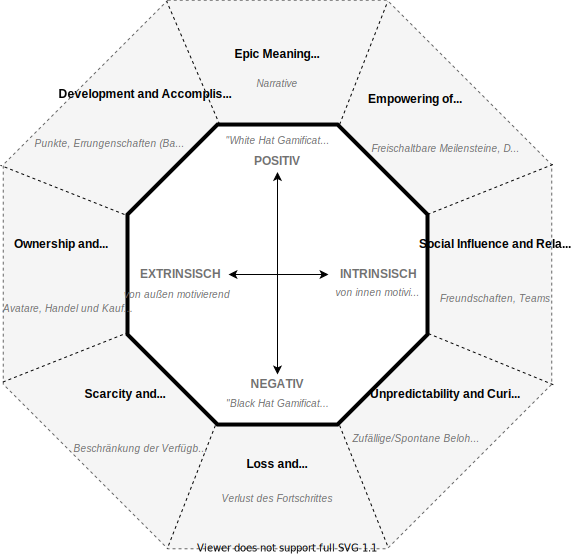
\includegraphics[width=0.75\linewidth, bb=0 0 408 402]{octalysis.pdf}
\caption{Die von Yu-kai Chou entwickelte Gamification-Taxonomie \enquote{Octalysis} als Oktagon mit beispielhaften Gamification-Elementen. Mit freundlicher Genehmigung \cite{chou_actionable_2019}.}\label{fig:octalysis}
\end{figure}

\noindent Weiterhin ordnet Chou diesen Teilzielen die jeweiligen Gamification-Elemente zu. So seien die weit verbreiteten Gamification-Elemente Punkte, Ranglisten und Errungenschaften (bspw. in Form von Badges) zuzuordnen in die Kategorie \enquote{Development and Accomplishment}. Die in \Cref{fig:octalysis} gezeigte Anordnung der acht Teilziele teilt Chou nochmals horizontal und vertikal. Die links in der Abbildung gezeigten Ziele zielten auf die durch äußere Reize hervorrufbare (extrinsische) Motivation des Nutzers ab, während die rechts gezeigten Ziele die von dem Nutzer selbst stammende (intrinsische) Motivation unterstützten. Außerdem seien die weiter oben angebrachten Ziele positiver als die weiter unten gezeigten Ziele, wie zum Beispiel \enquote{Loss and Avoidance}. Diese Teilung illustriert Chou als \enquote{White Hat Gamification} und \enquote{Black Hat Gamification}, was eine Analogie zum legalen White Hat Hacking und zum illegalen Black Hat Hacking darstellt. Eine nach diesen Zielen orientierte Gamification bezeichnet Chou als \enquote{Level 1 Octalysis}. Unter \enquote{Level 2 Octalysis} beschreibt er eine Gamification, welche die genannten Ziele der jeweiligen Phase des Spielers anpasst, wobei der Spieler das Spiel zunächst entdeckt, danach dessen Regeln erlernt und Ziele erreichen möchte und schließlich nach erreichen aller Ziele nach weiteren Motivationen sucht. Zusätzlich ließe sich hieran nach Chou die \enquote{Level 3 Octalysis} anschließen, die diese Faktorisierung der Spielphasen noch zusätzlich um eine Faktorisierung der Spielertypen erweitert.

\section{Softwarequalität}

In der folgenden Sektion werden die Grundlagen zum komplexen Begriff der Softwarequalität aufgeschlüsselt, um die Codequalität hierin schließlich systematisch einzuordnen und Möglichkeiten aufzuzeigen, diese in einem komplexen Softwaresystem abzubilden. Hierfür werden zunächst unterschiedliche Perspektiven erläutert, aus denen die Qualität einer Software betrachtet werden kann. Nachfolgend wird die Codequalität in eine dieser Perspektiven eingeordnet, um die Konsequenzen aus einer guten oder schlechten Codequalität für die Gesamtqualität der Software ableiten zu können und die Relevanz der Codequalität als zentrale Qualitätskomponente in der Gesamtqualität von Software zu zeigen. Außerdem wird beschrieben, wie deren Analyse über Codequalitätsmetriken funktionieren kann. Als zentraler Prozess in der Verbesserung von Softwarequalität wird schließlich der Vorgang der Refaktorisierung erklärt und mit dem Begriff der technischen Schulden in Verbindung gebracht sowie aufgezeigt, inwiefern dies automatisierbar ist.

\subsection{Komponenten und Faktoren}

Die Norm ISO/IEC 9126:2001 \cite{technical_committee_isoiec_jtc_1sc_7_software_and_systems_engineering_isoiec_2001}, aktualisiert durch ISO/IEC 25010:2011 \cite{technical_committee_isoiec_jtc_1sc_7_software_and_systems_engineering_isoiec_2011} beschreibt die Softwarequalität als komplexes Resultat aus dem Lebenszyklus von Software. Die Autoren unterteilen folgende Komponenten der Gesamtqualität von Software.

\begin{figure}[H]
\centering
\includegraphics[width=\linewidth, bb=0 0 549 277]{softwarequalitaet.pdf}
\caption{Die Kaskade der Softwarequalitätskomponenten im Lebenszyklus von Software und deren Modellindikatoren nach ISO/IEC 9126:2001 \cite{technical_committee_isoiec_jtc_1sc_7_software_and_systems_engineering_isoiec_2001}.}\label{fig:softwarequalitaet}
\end{figure}

\paragraph{Die Prozessqualität} beschreibt die Qualität der in ISO/IEC/IEEE 12207:2017 \cite{technical_committee_isoiec_jtc_1sc_7_software_and_systems_engineering_isoiecieee_2017} normierten Prozesse (Beschaffung, Lieferung, Entwicklung, Betrieb und Wartung) des Lebenszyklus einer Software.

\paragraph{Die interne und externe Qualität} wird von den Autoren beschrieben als die Charakterisierung der Software von einem internen bzw. externen Standpunkt, anhand der jeweiligen internen bzw. externen Anforderungen. \Cref{fig:softwarequalitaet} zeigt die in ISO/IEC 9126:2001 hierfür vorgeschlagenen Modellindikatoren (Funktionalität, Verlässlichkeit, Nutzbarkeit, Effizienz, Wartbarkeit und Portierbarkeit). Die interne Qualität wird hierbei über die Analyse der inneren Details der Software (Codebasis, statische und dynamische Modelle oder Dokumentation) festgestellt. Vice versa repräsentiert die externe Qualität die ohne Kenntnis dieser internen Details der Software messbare Qualität, beispielsweise durch funktionale Tests.

\paragraph{Die durch Nutzung der Software feststellbare Qualität} wird durch die Autoren definiert als die Fähigkeit der Software, die Bedürfnisse des Nutzers zu befriedigen. Sie separieren dies in die Effektivität, die Produktivität, die Sicherheit und die Zufriedenstellung bei der Nutzung.
\\

\noindent Weiterhin wird von den Autoren illustriert, dass sich die oben genannten Komponenten in dieser Reihenfolge im Lebenszyklus der Software kaskadierend gegenseitig beeinflussen (siehe \Cref{fig:softwarequalitaet}). So ist die durch Nutzung feststellbare Qualität von der externen Qualität abhängig, diese hängt wiederum von der internen Qualität ab und die interne Qualität wird schließlich beeinflusst von der Prozessqualität.

\subsection{Codequalitätsmetriken}

Die Codequalität lässt sich analog zum oben beschriebenen Schema in die interne Qualität der Software einordnen und kann nach den Kriterien der ISO/IEC 9126:2001 (Funktionalität, Zuverlässigkeit, Nutzbarkeit, Effizienz, Wartbarkeit und Wiederverwendbarkeit) \cite{technical_committee_isoiec_jtc_1sc_7_software_and_systems_engineering_isoiec_2001} beurteilt werden. Um die Konformität des Codes zu den Kriterien der internen Softwarequalität zu messen, werden typischerweise die Implementationen der einzelnen Teilkomponenten der Software anhand von bestimmten Metriken analysiert. Das grundlegende Prinzip solcher Metriken ist die Erkennung von Fehlgestaltungen verschiedener Art im Code und in dessen Dokumentation. Hierbei spielen oft der Umfang, die Komplexität und der Stil des Codes eine Rolle. Zusätzlich können Metriken eingesetzt werden, welche die Entwurfsqualität der Anwendung analysieren, zum Beispiel durch die Messung der Tiefe von Vererbungen in objektorientierten Anwendungen \cite{rosenberg_software_nodate}. Traditionelle Implementationen solcher Metriken umfassen hierzu beispielsweise die Berechnung der zyklomatischen Komplexität (McCabe-Metrik), die Bestimmung der Anzahl von Schachtelungen und Statements, die Kalkulation des Verhältnisses von Code und Kommentaren oder die Länge des Programms \cite{stamelos_code_2002}. Die Wahl, Funktionsweise und Interpretation der Metriken ist vom Kontext, zum Beispiel von der verwendeten Programmiersprache, von den Anforderungen der Software oder von der Erfahrung des Entwicklers, abhängig. Für unterschiedliche Kontexte lassen sich somit unterschiedliche Modelle zur Codequalitätsanalyse entwerfen, deren Wirkung aus der Zusammensetzung und Parametrisierung resultiert.

\subsection{Refaktorisierung}\label{sec:refaktorisierung}

Genügt die Codequalität einer Software nicht mehr den Anforderungen der Softwarequalitätsziele, so bietet sich eine Refaktorisierung an. Händler und Neumann definieren den Begriff wie folgt:

\begin{defs}
Unter Refaktorisierung versteht man die Verbesserung der internen technischen Qualität eines [Software]systems durch die Modifizierung und Restrukturierung des Quellcodes, ohne das von außen sichtbare Verhalten zu verändern. \cite{fowler_refactoring_1999}
\end{defs}

\noindent Das von außen sichtbare Verhalten ist hierbei vom Standpunkt und vom Kontext abhängig. Wird beispielsweise eine Software anhand ihrer nach außen verfügbaren Schnittstellen untersucht, so kann die interne Struktur mit Beibehaltung der äußeren Schnittstellen gänzlich verändert werden. Bei der Betrachtung einer einzelnen Komponente desselben Software-Systems, zum Beispiel anhand eines Unittests, muss die sichtbare Signatur der Komponente jedoch bei den Änderungen beibehalten werden, um nach der obigen Definition als Refaktorisierung zu gelten.

\subsection{Technische Schulden}

Um die Notwendigkeit der Refaktorisierung innerhalb einer jeweiligen Softwarekomponente zu quantifizieren, akkumulieren viele automatisierte Codeanalyseframeworks, wie zum Beispiel SonarQube\footnote{SonarQube. \url{https://www.sonarqube.org/} (Abgerufen am 14.9.2020)}, anhand einer Auswahl von Codequalitätsmetriken und anderen Metriken einen so genannten TD-Score\label{begriff:td-score}, wobei TD für \underline{T}echnical \underline{D}ebt (technische Schulden) steht. Der Score setzt sich hierbei metaphorisch zusammen aus der geschätzten Zeit, die zur Refaktorisierung der jeweiligen detektierten Fehlgestaltung notwendig wäre.

Die Art der Fehlgestaltungen kann hierbei jedoch stark variieren. Kruchten et al. unterteilen technische Schulden nochmals in Testschulden, menschliche Schulden, architekturelle Schulden, sich auf Abhängigkeiten beziehende Schulden, Dokumentationsschulden oder allumfassende amorphe Softwareschulden \cite{kruchten_technical_2012}. Kruchten et al. erklären darauf aufbauend, warum der errechnete TD-Score nicht mit den tatsächlichen technischen Schulden der Software gleichgesetzt werden sollte \cite{kruchten_technical_2012}. Die Gesamtheit von technischen Schulden sei nur schwierig durch statische Codeanalyseframeworks erfassbar, vor allem strukturelle und architekturelle Fehlgestaltungen. Zu beachten sei hierbei, dass sowohl die Codeanalyseframeworks als auch die zu analysierende Software dem technologischen Evolutions- und Alterungsprozess unterlägen.

\subsection{Codierungsrichtlinien}

Softwareentwickler können unterschiedliche Auffassungen von guter Codequalität haben. Hieraus lässt sich die Hypothese ableiten, dass Codequalitätsmetriken generell ungeeignet sind, um das Verständnis von guter Codequalität in allen Facetten zu modellieren. Pantiuchina et al. zeigten hierzu anhand eines Experimentes, dass die durch Metriken modellierbare Repräsentation von guter Codequalität nicht zwingend mit der Auffassung von Entwicklern übereinstimmt \cite{pantiuchina_improving_2018}.

Aus der Sicht des Entwicklers betrachtet, kann es, abhängig von der Zusammensetzung und Parametrisierung der Codequalitätsmetriken, zu falsch-positiven und falsch-negativen Detektionen kommen. Dies ist jedoch nicht immer von der individuellen Auffassung des Entwicklers abhängig. Händler und Neumann nennen hierzu den Fall, dass es auch bei bewusst auf eine bestimmte Art und Weise implementierten Strukturen, beispielsweise bei Entwurfsmustern, zu falsch-positiven Detektionen kommen kann. Sie begründen dies in der inhärenten Komplexität der Detektionsmechanismen \cite{haendler_serious_2019}.

\subsubsection{Konformität}

Jan Rucks befasste sich im Rahmen seiner Diplomarbeit mit der Auswahl von geeigneten Codequalitätsmetriken für das sich an die Lehrveranstaltung Softwaretechnologie zeitlich anschließende Softwarepraktikum, wo die Codequalität einiger Gruppen durch SonarQube analysiert wird \cite{rucks_erstellung_2017}. Wegen der oben genannten Schwierigkeiten ist es nicht verwunderlich, dass es Rucks nicht gelang, die Qualität einer Software (halb)-automatisch anhand einer Zusammenstellung von Qualitätsmetriken in Form einer einzigen Metrik zu messen.

Rucks evaluierte hierzu mehrere Metriken, welche bestimmte Teilaspekte der internen Softwarequalität modellieren sollen, darunter Flexibilität, Konformität, Sicherheit, Wiederverwendbarkeit, Testbarkeit, Modularität und Wartbarkeit. Rucks' Evaluation verglich dabei die Berechnungen der Metriken mit den Bewertungen der Tutoren zu der jeweiligen Gruppe sowie deren Selbsteinschätzung im Softwarepraktikum, um die Korrelation der Metriken mit der Softwarequalität zu bestimmen. Hierbei sei angemerkt, dass sowohl die Bewertungen der Tutoren als auch die Selbsteinschätzung der Gruppen gute Codequalität nicht ideal repräsentieren, was die Aussagekraft der darauf fußenden Evaluation beschränkt. Rucks destillierte aus der Evaluation dennoch als einzige signifikant mit den jeweiligen Einschätzungen der Gruppe korrelierende Metrik die der Konformität, welche sich wie folgt berechnen lässt:

\begin{equation}\label{eq:konformitaetsmetrik}
M_{CON} = 1 - \frac{N_{BLV} * 2 + N_{CRV} * 1,5 + N_{MAV} + N_{MIV} * 0,5}{N_{STA}}
\end{equation}
wobei:
\begin{conditions}
    M_{CON} & Konformitätsmetrik \\
    N_{BLV} & Anzahl der Verletzungen von \enquote{Blocker}-Regeln \\
    N_{CRV} & Anzahl der Verletzungen von \enquote{Critical}-Regeln \\
    N_{MAV} & Anzahl der Verletzungen von \enquote{Major}-Regeln \\
    N_{MIV} & Anzahl der Verletzungen von \enquote{Minor}-Regeln \\
    N_{STA} & Anzahl von Statements
\end{conditions}

\noindent Analog zu den Teilkomponenten der in \Cref{eq:konformitaetsmetrik} beschriebenen Konformitätsmetrik berechnet sich diese aus dem Verhältnis der gewichteten Anzahl an Verletzungen von Codierungsrichtlinien zu der Gesamtanzahl an Statements. Die Gewichtung stammt vom durch SonarQube kategorisierten Schweregrad der jeweiligen Verletzung der Codierungsrichtlinien, von der schwerwiegendsten Art \enquote{Blocker}, über \enquote{Major}, \enquote{Minor} bis hin zur Einstufung als \enquote{Info}. Die Beobachtung, dass die Konformität, also die Einhaltung von bestimmten Codierungsrichtlinien, die Codequalität signifikant positiv beeinflusst, beschreiben auch Dietz et al \cite{dietz_teaching_2018}. Durch die Einhaltung solcher Richtlinien würde die Lesbarkeit des Codes erhöht und hierdurch dessen Wartbarkeit verbessert. Als Konsequenz hieraus verringerten sich die Wartungskosten der Software.

% - Wang et al.: systematische Literaturreview

\subsubsection{Detektion von Code Smells}\label{sec:code-smells}

Mithilfe einer fundierten Auswahl von Codierungsrichtlinien ist es möglich, eine gegebene Software auf potenzielle Verstöße gegen diese Codierungsrichtlinien zu prüfen und dem Entwickler verständlich aufzuzeigen. Die detektierten Verstöße werden hierbei oft als \enquote{Code Smells}, also sinngemäß \enquote{schlechte Gerüche} bezeichnet. Als Synonym werden Code Smells auch einfach als \enquote{Smells} oder präziser als Refaktorisierungskandidaten bezeichnet. Die Analyse der Code Smells läuft hierbei ohne einen tatsächlichen Start der Anwendung, weshalb diese Technik auch als statische Codeanalyse bezeichnet wird. Tools wie Checkstyle\footnote{Checkstyle. \url{https://checkstyle.sourceforge.io/} (Abgerufen am 13.6.2020)}, PMD\footnote{PMD. \url{https://pmd.github.io/} (Abgerufen am 13.6.2020)} und FindBugs\footnote{FindBugs. \url{http://findbugs.sourceforge.net/} (Abgerufen am 13.6.2020)}/SpotBugs\footnote{SpotBugs. \url{https://spotbugs.github.io/} (Abgerufen am 14.9.2020)}\footnote{FindBugs wird nicht mehr weiterentwickelt und wurde durch SpotBugs ersetzt.} verwenden Pattern Matching, um Code Smells anhand von bestimmten Mustern zu finden und so dem Entwickler zusätzlich zu den meist bereits vom Compiler bereitgestellten Warnungen Hinweise auf potenzielle Degradationen der Codequalität zu geben. Wegen der großen Variabilität der zugrunde liegenden Codierungsrichtlinien gibt es eine Vielzahl von möglichen Unterteilungen von Code Smells. Fowler et al. unterteilen Code Smells beispielsweise in 22 Kategorien \cite{fowler_refactoring_1999}.

\subsubsection{Automatisierung}

Mithilfe einer automatisierten Detektion von Refaktorisierungskandidaten können Degradationen der Codequalität frühzeitig erkannt und behoben werden. In kontinuierlich evolvierenden Softwareprojekten und vor allem bei iterativen Projektmanagement-Strategien wie SCRUM \cite{gloger_scrum_2016} oder dem Spiralmodell \cite{boehm_spiral_1988} repräsentiert die Refaktorisierung als Entwicklungsschritt einen großen Zeitaufwand, wobei die einzelnen Refaktorisierungsmaßnahmen repetitiv erscheinen mögen. Zur Mitigation dieses Problems haben sich einige Ansätze etabliert, zum Beispiel Autofactor \cite{rouvignac_httpautorefactororg_2020}, WalkMod \cite{pau_httpwalkmodcom_2020}, Facebooks pfff \cite{facebook_httpsgithubcomfacebookarchivepfff_2020}, Kadabra \cite{bispo_httpsgithubcomspecs-feupkadabra_2020} oder Leafactor \cite{cruz_leafactor_2017}. Diese Tools detektieren Refaktorisierungskandidaten und beheben diese soweit möglich. Zur Vereinfachung können die Tools dabei teilweise in Entwicklungsplattformen integriert oder über eigene Programmierschnittstellen angesprochen werden. Dennoch ist der Handlungsfreiraum dieser Tools durch die Komplexität der Detektionsmechanismen und der zu refaktorisierenden Software beschränkt. Eine automatisierte Refaktorisierung ist hierdurch mit weiteren Problemen behaftet, zum Beispiel durch die transitive Induzierung von weiteren Refaktorisierungskandidaten in den Programmcode durch die Behebung eines einzelnen Refaktorisierungskandidaten (für ein konkretes Beispiel siehe \Cref{sec:code-smell-quiz}). Durch die Beschränktheit der automatisierten Refaktorisierung kann diese infolgedessen die manuelle Refaktorisierung nicht vollständig ersetzen, aber dennoch als hilfreiches Werkzeug bei der Entwicklung dienen.


\section{Zusammenfassung}

Im E-Learning-System INLOOP können Studierende interaktiv Programmieraufgaben lösen und erhalten ein direktes Feedback über die funktionelle Korrektheit der eingereichten Lösungen. Neben der funktionellen Korrektheit trägt auch die Codequalität maßgeblich zur Gesamtqualität der Software bei. Dabei ist die eindeutige Erkennung von guter Codequalität sowohl für Entwickler, als auch für automatisierte Metriken schwierig und komplex. Es wurde noch keine Metrik gefunden, die eine gute Codequalität vollständig abbildet. Die Metrik der Konformität scheint allerdings signifikant mit der Codequalität zu korrelieren. Durch die Verbesserung der Lesbarkeit und Wartbarkeit scheint Software, die einem festen Regelwerk mit Codierungsrichtlinien entspricht, in der Regel eine höhere Codequalität zu besitzen, als Software, die diesem nicht entspricht. Für die Detektion von Verstößen gegen diese Richtlinien können Tools zur statischen Codeanalyse verwendet werden, um potenzielle Verstöße (Code Smells) gegen die festgelegten Codierungsrichtlinien zu detektieren und hierüber die Konformitätsmetrik gewichtet zu aggregieren. Studierende könnten zur Erhöhung der Codequalität motiviert werden, die zugrundeliegenden Codierungsrichtlinien einzuhalten und Verstöße gegebenenfalls zu refaktorisieren. Als in unterschiedlichen Domänen erfolgreicher Motivator etablierte sich das Prinzip der Gamification, welches durch die Einführung von über ein Game-Design miteinander verknüpften Gamification-Elementen auf die Erfüllung von psychologischen Bedürfnissen abzielt. Anhand des Octalysis-Ansatzes wurde beschrieben, welche Faktoren bei einem nutzerzentrierten Game-Design zu beachten sind und wie diese wirken. In diesem Rahmen wurde gezeigt, wie unterschiedliche Game-Design-Elemente intrinsisch oder extrinsisch wirken können und wann diese als positiv oder negativ empfunden werden.


  \chapter{Related Work}\label{ch:related-work}

Im folgenden Kapitel werden verschiedene verwandte Ansätze aus der Domäne der Gamification diskutiert, deren direktes oder indirektes Ziel die Verbesserung der Codequalität im universitären Kontext ist. Einen allgemeinen Überblick über die Gamification im Software Engineering zeigen die systematischen Studien von Pedreira et al. \cite{pedreira_gamification_2014} und von Alhammad und Moreno \cite{alhammad_gamification_2018}, Letztere mit dem für diese Arbeit relevanten didaktischem Fokus. Obwohl Alhammad und Moreno anhand der systematischen Analyse Gamification als vielversprechendes Prinzip für die Verbesserung der Lehre der Softwareentwicklung einschätzen, gibt es zur Applikation von Gamification in diesem Kontext nur wenig empirische Forschung \cite{alhammad_gamification_2018}. Campolina et al. analysierten die Gründe hinter der geringen Verbreitung von Gamification in diesem Kontext \cite{campolina_games_2018}. Außerdem lässt sich beobachten, dass einige der Ansätze, Gamification in der Lehre der Softwareentwicklung einzusetzen, andere Schwerpunkte als die Codequalität behandeln, beispielsweise das Requirements Engineering \cite{mei_teng_game-based_2018}\cite{campolina_games_2018}, den Scrum-Prozess \cite{neto_case_2019}, die Integration von Peer-Review-Konzepten \cite{indriasari_gamification_2020}\cite{berkling_presenting_2019}, die Verbesserung von hochintensiven Programmierkursen \cite{akpolat_enhancing_2014} oder die Motivation von Softwaretests \cite{rojas_code_2016}\cite{sheth_halo_2011}. Nennenswert ist auch der eher unkonventionelle Ansatz von Baars und Meester, die ein Java-Refaktorisierungsspiel in Minecraft integrierten \cite{baars_codearena_2019}. Elezi et al. zeigen eine Anwendung von Gamification zur Motivation der Refaktorisierung von Code \cite{elezi_game_2016}, allerdings nicht in einem akademischen Kontext, sondern mit praxiserfahrenen Softwareentwicklern.

Dos Santos et al. kamen daher 2019 nach deren Einschätzung zu dem Schluss, dass ihre Arbeit die erste wissenschaftliche Kontribution im Bereich der Motivation zur Refaktorisierung von Code Smells durch Gamification im akademischen Kontext ist \cite{dos_santos_cleangame_2019}. Nachfolgend wird zunächst das von dos Santos et al. als \enquote{CleanGames} bezeichnete Konzept diskutiert. Anschließend wird ein verwandter Ansatz von Händler und Neumann beschrieben, der die Motivation der Refaktorisierung von Code über Serious Games behandelt \cite{haendler_serious_2019}. Zur Erkennung von Refaktorisierungskandidaten eignet sich die statische Codeanalyse. Mit Fokus auf diese beschäftigen sich Dietz et al. mit der Frage, wie Codequalität gelehrt werden kann, um schließlich eine Grundlage für die automatisierte Codequalitätsanalyse in einem universitären Kontext zu konzeptionieren \cite{dietz_teaching_2018}. Dieser Ansatz wird in der abschließenden Sektion diskutiert.


\section{CleanGame: Gamifying the Identification of Code Smells}\label{sec:cleangame}

Wie in \Cref{sec:refaktorisierung} bereits näher beschrieben, bietet die Refaktorisierung eine Möglichkeit, die Softwarequalität zu verbessern, indem interne Komponenten abgeändert werden, während die externe Funktionalität unverändert bleibt. Dieser Prozess inkludiert eine systematische Suche und Behandlung von Refaktorisierungskandidaten. In welchem Maße eine Refaktorisierung durchgeführt werden kann und wie erfolgreich diese der Softwarequalität zugutekommt, hängt somit auch von der Menge und der Sinnhaftigkeit der gefundenen Refaktorisierungskandidaten ab. Auf Grundlage dieser Prämisse untersuchten dos Santos et al., wie die Suche von Refaktorisierungskandidaten in einem akademischen Kontext durch Gamification spielerisch motiviert werden kann und welche quantitativen Auswirkungen dies auf die Fähigkeit der Nutzer, Refaktorisierungskandidaten zu finden, haben kann \cite{dos_santos_cleangame_2019}.

\subsection{Game-Design}

Die von den Forschern hierzu entworfene Webanwendung trägt den Namen \enquote{CleanGame} und besteht aus einem Quiz über Code Smells und einem Spiel, bei dem Refaktorisierungskandidaten in Codeschnipseln gefunden werden sollen. Über das Quiz sollen die Kernkonzepte der Refaktorisierung reflektiert werden, während durch das andere Modul die Suche nach Refaktorisierungskandidaten trainiert werden soll. Das Softwaretool lässt sich in die Kategorie der Serious Games einordnen.

\subsubsection{Code-Smell-Quiz}\label{sec:code-smell-quiz}

Im Code-Smell-Quiz werden dem Nutzer Fragen zu ausgewählten Code-Smells gestellt. Die Forscher fokussieren sich hierbei auf die folgenden fünf konkreten Code-Smells, basierend auf einer Metaanalyse von Code Smells im akademischen und industriellen Kontext von Sharma und Spinellis \cite{sharma_survey_2017}:

\begin{enumerate}
\item \textbf{Large Class}: Hierunter fallen Klassen, welche zu viele Verantwortlichkeiten tragen. Dieses Anti-Pattern ist auch bekannt unter den Namen \enquote{Blob} oder \enquote{Gott-Klasse} \cite{sourcemakingcom_design_2020}.
\item \textbf{Long Method}: Dies bezeichnet Methoden, welche zu viele Zeilen von Code beinhalten.
\item \textbf{Divergent Change}: Hiermit beschreiben die Autoren eine Klasse, die sich im Verlauf der Entwicklung häufig und aus verschiedenen Gründen ändert.
\item \textbf{Feature Envy}: Unter diesem Namen werden Klassen kategorisiert, welche deren Funktion hauptsächlich durch die Kommunikation mit anderen Klassen realisieren, also kaum eigene Funktionalität bereitstellen. Häufig steht dieses Anti-Pattern in Verbindung mit der Auslagerung von Daten-Klassen \cite{refactoringguru_data_2020}.
\item \textbf{Shotgun Surgery}: Durch diese Bezeichnung beschreiben dos Santos et al. Modifikationen in Klassen, welche viele kleine Änderungen in anderen Klassen hervorrufen.
\end{enumerate}

\noindent Innerhalb des Quiz werden dem Nutzer Fragen zu diesen fünf Kategorien gestellt, wobei die Antwortmöglichkeiten festgelegt sind. Um den Frageprozess zu illustrieren, zeigen dos Santos et al. folgende Frage inklusive deren Antwortmöglichkeiten:

\begin{quote}
Um den Shotgun Surgery Code Smell zu beseitigen, können Refaktorisierungen verwendet werden. Welche der folgenden Refaktorisierungen würden Sie nutzen, um dies zu realisieren?

\begin{itemize}
\item[A] Vererbung mit einer Delegation ersetzen
\item[B] Inline Class
\item[C] Methoden extrahieren
\item[D] Klasse extrahieren
\end{itemize}
\cite[sinngemäß übersetzt. S. 4, Abb. 1]{dos_santos_cleangame_2019}
\end{quote}

\noindent Um diese Frage, ohne zu raten, erfolgreich zu lösen, muss der Nutzer ein komplexes, vernetztes Fachwissen über Code Smells und Refaktorisierung besitzen. Zunächst muss der Nutzer wissen, worum es sich bei der \enquote{Shotgun Surgery} handelt und, dass das zugrundeliegende Problem dieses Anti-Patterns die Zersplitterung einer Verantwortlichkeit über verschiedene Klassen ist \cite{refactoringguru_shotgun_2020}. Eine Möglichkeit der Refaktorisierung wäre die Extraktion von zur Verantwortlichkeit gehörenden Methoden aus den verschiedenen Klassen und deren Reintegration in eine zentrale Klasse. Somit wäre Antwortmöglichkeit C bereits richtig. Durch die Migration der Methoden können jedoch auch Klassen entstehen, welche selbst keine Verantwortlichkeiten mehr besitzen. Diese Klassen werden als \enquote{Inline Class} \cite{refactoringguru_inline_2020}, meist auch als \enquote{Data Class} bezeichnet und fallen unter die Kategorie \enquote{Feature Envy}. Richtig wäre also auch Antwortmöglichkeit B, um die möglichen transitiven Konsequenzen aus der initialen Refaktorisierung zu behandeln. Dieses Beispiel illustriert, wie über den Ansatz der Autoren über ein Quiz komplexes vernetztes Fachwissen zur Refaktorisierung abgefragt, reflektiert und erlernt werden kann.

\subsubsection{Verwendete Gamification-Elemente}

Während des Quiz erhält der Nutzer Punkte für das richtige Beantworten einer Frage. Für das falsche Beantworten einer Frage bekommt der Nutzer Punkte abgezogen. Noch während des Quiz kann der Nutzer den durch seinen aktuellen Punktestand errechneten Rang in der Rangliste einsehen. Für eine Frage hat der Nutzer nur begrenzt Zeit zur Verfügung. Fragen können übersprungen werden, während Schnelligkeit bei deren Beantwortung durch einen Zeitbonus belohnt wird. Beantwortet der Nutzer einige aufeinander folgende Fragen richtig, so erhält er auch hierfür Bonuspunkte. Weiterhin sieht der Nutzer seinen eigenen Fortschritt über einen Fortschrittsbalken in der Webanwendung. Der Nutzer hat, nach \cite[S. 4, Abb. 1]{dos_santos_cleangame_2019} außerdem die Möglichkeit, sich zu registrieren und für den erstellten Account einen rudimentären Avatar anzulegen.

\subsubsection{Code-Smell-Suche}

Bei der zweiten Kernkomponente von CleanGame handelt es sich um eine Code-Smell-Suche, bei der dem Nutzer Code-Schnipsel gezeigt werden, zu denen er den passenden Code Smell aus einer festen Auswahl von Code Smells selektieren soll. Die Code-Smell-Suche ähnelt dem Quiz in deren Aufbau und Funktionsweise, denn auch hier erhält der Nutzer Punkte für richtige Antworten und bekommt Punkte für falsche Antworten abgezogen. Dies wird erweitert durch die Fähigkeit des Nutzers, die Punkte als Währung gegen Tipps einzutauschen. Ein Tipp kann die Angabe von Regeln sein, die mit dem Code Smell in Verbindung stehen, oder eine Einschränkung des zu betrachtenden Codeabschnittes, oder die dem Code Smell zugrundeliegende Definition.

\subsection{Ergebnisse}

Dos Santos et al. prüften ihr Konzept im akademischen Kontext anhand einer quantitativen Analyse über die Messung der durch die Probanden gefundenen Code Smells und einer qualitativen Analyse der persönlichen Einstellung der Nutzer gegenüber dem Game-Design. Bei der quantitativen Analyse zweier randomisierter Nutzergruppen, wobei die eine Nutzergruppe CleanGame und die andere Nutzergruppe eine IDE im Voraus zum Training der Identifikation von Code Smells nutzte, konnten die Nutzer der CleanGame-Gruppe nach dem Training doppelt so viele Code Smells identifizieren, wie Nutzer der IDE-Gruppe. Für die Selektion der Trainingsbeispiele und der Evaluationsbeispiele nutzten dos Santos et al. validierte Code Smells der Plattform \enquote{Landfill} \cite{palomba_landfill_2015}. In einer qualitativen Analyse über eine Umfrage ermittelten dos Santos et al., dass die Attitüde der Probanden gegenüber dem evaluierten Serious Game überwiegend positiv war. Als verbesserungswürdig schätzten Probanden unter anderem vor allem Probleme mit der Benutzeroberfläche ein, aber auch, dass kein direktes Feedback über die richtige Antwort einer Frage gegeben wurde und, dass die Punkte eines jeweiligen Nutzers öffentlich einsehbar waren. Als positiv schätzen die Probanden wiederum unter anderem vor allem die spielerische und interaktive Auseinandersetzung mit dem Thema ein sowie die Unterstützung beim Verstehen von Code Smells und die Kompetitivität. Die qualitative Evaluation der ästhetischen Wahrnehmung des Tools ergab weiterhin, dass durch den Ansatz der Autoren die Relevanz, die Lernwahrnehmung und die soziale Interaktion besonders betont würde.

\noindent Die Autoren interpretieren diese Ergebnisse als Unterstützung der Hypothese, dass Gamification in diesem Kontext geeignet ist. Zu berücksichtigen ist jedoch, dass sowohl die qualitative als auch die quantitative Analyse nur mit 18 Probanden durchgeführt wurden und somit nur bedingt aussagekräftig sind. Daher merken dos Santos et al. an, dass die Ergebnisse weiterhin validiert werden müssen, um eine hinreichende Konfidenz über die Wirksamkeit des Effekts der Gamification im universitären Kontext zur Motivation von Refaktorisierung zu erhalten.

\section{Serious Refactoring Games}\label{table:bloom-taxonomy-serious}

Die Refaktorisierung von Code mit Hinblick auf die Verbesserung der Codequalität ist ein komplexer Prozess. Ein zu dem vorgestellten \enquote{CleanGame} Konzept ähnliches Serious Game konzipierten Händler und Neumann. Die Autoren betrachten die didaktische Komplexität der Refaktorisierung von Code anhand der Taxonomie von Bloom \cite{bloom_taxonomy_1956}\cite{anderson_taxonomy_2000}, welche Denkfähigkeiten geordnet nach der mentalen Beanspruchung, von \enquote{lower order thinking skills} wie dem Merken von Informationen bis hin zu \enquote{higher order thinking skills} wie der Evaluation und der Kreation kategorisiert. Händler und Neumann kommen dabei zu dem Ergebnis, dass die Refaktorisierung von Code alle der Kategorien in Blooms Taxonomie beansprucht \cite{haendler_serious_2019}. Diese Aufschlüsselung ist in \Cref{tab:bloom} gezeigt.

\begin{table}[H]
\caption{Kognitive Fähigkeiten bei der Refaktorisierung anhand von Blooms Taxonomie. Sinngemäß aus der tabellarische Darstellung in \cite[S. 3]{haendler_serious_2019} abstrahiert.}\label{tab:bloom}
\begin{tabularx}{\textwidth}{{
    >{\hsize=.5\hsize\linewidth=\hsize}X
    >{\hsize=1.5\hsize\linewidth=\hsize}X
}}
\hline
Stufe in Blooms Taxonomie & Beispiel für eine benötigte Fähigkeit bei der Refaktorisierung \\ \hline \hline
1. Wissen & Die Regeln und Schritte für die Planung und die Durchführung der Refaktorisierung kennen. \\ \hline
2. Verstehen & Die Regeln und Schritte für die Planung und die Durchführung der Refaktorisierung verstehen. \\ \hline
3. Applikation & Die Regeln und Schritte für die Planung und die Durchführung der Refaktorisierung anwenden. \\ \hline
4. Analyse & Den Quellcode eines Systems analysieren und hieraus Kandidaten für die Refaktorisierung ableiten. \\ \hline
5. Bewertung & Mehrere Möglichkeiten der Refaktorisierung von Refaktorisierungskandidaten miteinander vergleichen und sich für die bestmögliche Lösung entscheiden. \\ \hline
6. Kreation & Entwicklung und Verbesserung von Systemen und Arbeitsweisen, welche die Refaktorisierung von Softwaresystemen vereinfachen oder strukturieren. \\
\hline
\end{tabularx}
\end{table}

Anhand dieser Erkenntnis kritisieren die Autoren, dass bisherige didaktische Lösungen für die Lehre des Refactorings nur künstliche, kleine Aufgaben beinhalten, die aber nicht ausreichend seien, um tiefergehende Kompetenzen wie analytisches Denken und die Bewertung von Lösungen zu vermitteln. Stattdessen schlagen sie ein Spiel vor, bei dem dem Nutzer ein größeres, in dessen Kontext funktionales, Codefragment präsentiert wird und es daraufhin des Nutzers Aufgabe ist, die in diesem Codefragment vorhandenen Code Smells zu beseitigen, ohne die von außen erkennbare Funktionalität abzuändern. Hierbei kann der Nutzer gegen einen Codequalitätsbenchmark (Technische Schulden) oder gegen echte Mitspieler antreten. In diesem Kontext beschreiben Händler und Neumann eine technische Grundlage für das Game-Design solcher \enquote{Serious Refactoring Games} auf Basis von existierenden Codeanalyse-Tools (Test-Frameworks, Softwarequalitätsmetriken) und Regressionstests.

Die vorgeschlagene Lösung von Händler und Neumann hat das Ziel, insbesondere auch die höherliegenden Stufen 3-6 der Taxonomie von Bloom (\Cref{table:bloom-taxonomy-serious}) didaktisch zu vermitteln, da sich existierende Lösungen eher auf die darunter liegenden Stufen orientierten, analysieren die Autoren. Durch die Konfrontation mit Codefragmenten aus \enquote{echten} Anwendungen werde eine praxisnähere Situation simuliert, bei der Nutzer die Artefakte zunächst analysieren müssen und danach Alternativen evaluieren müssen, um die Code Smells zu beseitigen, wodurch höhere Lernziele in Blooms Taxonomie repräsentiert würden.

\subsection{Game-Design}

Der Spieler erhält den Quellcode der zu refaktorisierenden Datei(en). Des Spielers Aufgabe ist es hiernach, den Quellcode auf mögliche zu refaktorisierende Stellen (Refaktorisierungskandidaten) zu untersuchen und diese auszuwählen. Wenn der Spieler einen oder mehrere Kandidaten ausgewählt hat, muss er Modifikation(en) des Quellcodes planen und ausführen, die den jeweiligen ausgewählten Kandidaten behandelt. Signalisiert der Spieler, dass dieser die Modifikation(en) abgeschlossen hat, wird die editierte Datei im ursprünglichen System integriert und auf Funktionalität geprüft (Regressionstest). Nun kann es zwei Ergebnisse dieser Interaktion geben:

\begin{itemize}
\item Der Programmcode ist valid und alle Regressionstests waren erfolgreich. Infolgedessen wird die Qualität des refaktorisierten Codes analysiert und ein Score für die technischen Schulden ermittelt.
\item Einer oder mehrere Regressionstest schlagen fehl oder der Programmcode ist anderweitig invalid. Die Qualität des refaktorisierten Codes wird nicht analysiert und es wird kein Score für die technischen Schulden ermittelt.
\end{itemize}

\noindent Das ermittelte Ergebnis wird dem Spieler präsentiert und dieser erhält, wenn vorhanden, den zum refaktorisierten Code berechneten Score. Der Spieler erhält nun die Option, weitere Modifikationen an den bereits ausgewählten Kandidaten vorzunehmen oder nach weiteren Kandidaten zu suchen. Das Spiel ist nach dem beschriebenen Ablauf in Spielzüge unterteilt, welche nach deren Abschluss als inkorrekt, korrekt oder erfolgreich gelten können:

\begin{itemize}
\item Inkorrekt: der Quellcode ist invalid und konnte nicht auf Funktionalität oder Qualität geprüft werden.
\item Korrekt: der Quellcode ist valid, die technischen Schulden haben sich aber im Vergleich zum vorigen Spielzug nicht verringert.
\item Erfolgreich: der Quellcode ist valid und die technischen Schulden haben sich im Vergleich zum vorigen Spielzug verringert.
\end{itemize}

\noindent Händler und Neumann schlagen mehrere erweiterte Spielmodi vor, darunter ein Einzelspielermodus, wobei der Spieler gegen die Uhr spielt sowie mehrere Mehrspielermodi (parallel vs. alternierend, kompetitiv vs. kollaborativ).

\subsubsection{Ziele eines Serious Refactoring Games}

Das oberste Ziel des Spielers besteht darin, das Codefragment auf eine solche Weise zu refaktorisieren, sodass die Funktionsfähigkeit der Software weiterhin durch die Regressionstests verifiziert werden kann, sich in diesem Kontext also nach außen nicht verändert, während die technischen Schulden minimiert werden.

\subsubsection{Technische Realisation}

Das von Händler und Neumann konzipierte Softwaresystem ist in die folgenden Komponenten unterteilt:

\begin{itemize}
\item Die \textbf{Game Control} koordiniert die Interaktion von Spielern und dem Testframework bzw. der Qualitätsanalyse.
\item Das \textbf{Test Framework} führt Regressionstests auf der eingereichten Software aus.
\item Der \textbf{Quality Analyzer} analysiert die Qualität des Codefragments.
\item Die \textbf{GUI Component} kapselt das visuelle Feedback und die gesamte visuelle Interaktion.
\end{itemize}

\noindent Als Grundlage schlagen Händler und Neumann eine Messung der internen technischen Qualität über die Akkumulation eines TD-Scores (\Cref{begriff:td-score}) vor.

\subsection{Ergebnisse}

Händler und Neumann planen die Evaluation des vorgestellten Konzeptes im universitären Kontext im Rahmen zukünftiger Arbeit \cite[S. 9]{haendler_serious_2019}. Zu dem vorgestellten Konzept der Serious Refactoring Games wurden noch keine experimentellen Resultate publiziert (Stand: 30. Juni 2020), so auch nicht in der in \cite{haendler_interactive_2019} von Händler et al. auf Grundlage dessen fortgeführten Arbeit, welche sich im Kontrast zu den vorgestellten Serious Refactoring Games auf die Realisation der Interaktivität über ein direktes Feedback im Rahmen eines Tutoring-Systems fokussiert.

\subsection{Framework}\label{sec:haendler-framework}

In \cite{haendler_framework_2019} diskutieren Händler und Neumann die Serious Refactoring Games und das oben genannte Tutoring-System erneut und konzipieren anhand dessen ein Framework, welches die Lernziele in Blooms Taxonomie möglichst gut abbildet. Hierbei soll das vorgestellte Serious Refactoring Game durch folgende Konzepte aus dem Tutoring-System komplementiert werden:

\begin{itemize}
\item Die Bereitstellung von direktem, interaktiven Feedback durch die Präsentation der Resultate von Regressionstests.
\item Der interaktive Vergleich des durch den Code zu reflektierenden Referenz-UML-Diagramms (Soll-Zustand) mit einem aus dem eingereichten Code ermittelten UML-Diagramm (Ist-Zustand).
\end{itemize}

\noindent Ähnlich zu den in \Cref{sec:cleangame} beschriebenen CleanGames soll hierdurch ein weiterer Spielmodus umgesetzt werden, dessen Ziel die Eliminierung von Code Smells aus einem gegebenen Codefragment ist, während die Regressionstests auf eine fortexistierende Funktionalität und damit die Validität der Refaktorisierung prüfen. Als eine weitere Möglichkeit zur Ergänzung des Frameworks nennen Händler und Neumann die Integration eines Quiz über Refaktorisierung, ähnlich dessen in CleanGames, welches in \Cref{sec:cleangame} näher beschrieben wurde.


\section{Teaching Clean Code}

Dietz et al. befassten sich mit den Forschungsfragen, wie die Programmierung von \enquote{Clean Code}, also Code mit hoher Konformität zu Codierungsrichtlinien, in einem universitären Kontext gelehrt werden kann und wie dies mit einer zunehmenden Anzahl an Studierenden skalierbar umsetzbar ist. Dazu gehen die Autoren auf Probleme ein, die in der Lehre von Clean Code im universitären Kontext bestehen. Über die Integration eines didaktischen Konzeptes auf Grundlage von persönlichem Feedback sammelten Dietz et al. Erkenntnisse über die Strukturierung und Auswahl von Codierungsrichtlinien. Mithilfe dieser empirischen Auswahl wird schließlich eine Grundlage für deren Integration in einem E-Learning-System wie ArTEMiS \cite{krusche_artemis_2018}, einem INLOOP ähnelnden E-Learning-System für Softwaretechnologie der Technischen Universität München, mit Fokus auf der Verbesserung der Codequalität gegeben.

\subsubsection{Herausforderungen in der universitären Lehre}

Dietz et al. beschreiben, dass Studierende der Informatik häufig aufgrund der Lehrstruktur des Studiengangs nicht ausreichend motiviert würden, sich über die praktische Applikation von theoretischen Konzepten hinweg autodidaktisch mit der qualitativen Verbesserung des eigenen Codes zu befassen, weil dieser oft nach der Entwicklung vergessen oder \enquote{weggeworfen} würde. Motiviert hierdurch analysierten Dietz et al., wie die Einhaltung von Codierungsrichtlinien in einem universitären Kontext, ähnlich dem dieser Arbeit, gelehrt werden kann. So integrierten sie ein didaktisches Konzept in den Präsenzbetrieb einer Lehrveranstaltung mit den folgenden drei Kernelementen:

\begin{itemize}
\item Interaktive Diskussion von Refaktorisierungskandidaten in der Vorlesung zwischen den Studierenden und dem Vorlesenden anhand von Lösungen zu Aufgaben
\item Detaillierte Code Reviews von Lösungen der Übungsgruppen durch Lehrpersonal
\item Integration einer Aufgabenstellung in die mündliche Prüfung, bei der Refaktorisierungskandidaten in einem unbekannten Code-Schnipsel erkannt werden sollen
\end{itemize}

\noindent Dieses didaktische Konzept erprobten die Autoren an der Universität Bamberg mehrere Jahre und evaluierten schließlich mithilfe von statischer Codeanalyse die messbaren Änderungen in der Konformität des eingereichten Codes zu einem festen Regelwerk. Sie stellten als Tendenz fest, dass sich die allgemeine Struktur des Codes verbesserte, während andere Regelverstöße zunahmen, wobei die Autoren diese Zunahmen teilweise der Art der Aufgabe attribuieren \cite[S. 3]{dietz_teaching_2018}.

Bei diesem Konzept spielen die personellen Ressourcen eine große Rolle, so dass bei der Umsetzung jedes der drei Kernelemente Lehrpersonal vonnöten ist. Mit einer steigenden Teilnehmerzahl in den Informatik-Studiengängen steigt damit auch der Bedarf an den personellen Ressourcen zur Umsetzung eines solchen Konzeptes, wodurch der Bedarf einer skalierbareren Lösung entsteht.

\subsubsection{Auswahl von Codierungsrichtlinien}\label{sec:qualityreview}

Um die Skalierbarkeit des Konzepts zu verbessern, schlagen Dietz et al. vor, die Erfahrungen aus der Umsetzung des Konzepts in eine Wissensbasis zu überführen \cite{dietz_teaching_2018} und auf Grundlage dieser eine automatisierte statische Codeanalyse durchzuführen. Die Autoren verfassten die Wissensbasis als Buch unter dem Titel \enquote{Java by Comparison: Become a Java Craftsman in 70 Examples.} mit den am weitesten verbreiteten Problemen inklusive Codebeispielen und Erklärungen \cite{harrer_java_2018}.

Anhand der universitären Wissensbasis erstellten die Autoren ein Meta-Tool, welches in Summe etwas mehr als 100 Regeln der Codeanalyseframeworks Checkstyle, PMD und FindBugs/SpotBugs kombiniert und genutzt werden kann, um Codierungsrichtlinien, welche sich für einen universitären Kontext eignen, automatisiert in E-Learning-Systeme zu integrieren. Bei der Zusammenstellung der Richtlinien verfolgen Dietz et al. die Maxime, diese möglichst sinnvoll für alle Lerntypen auszuwählen und die Anzahl der falsch-positiven Detektionen gering zu halten. Bestimmte Programmierstile sollen darüber hinaus nicht forciert werden. Das entwickelte Meta-Tool ist unter dem Namen QualityReview auf GitHub\footnote{QualityReview. \url{https://github.com/LinusDietz/QualityReview} (Abgerufen am 13.6.2020)} verfügbar und beinhaltet Regelsätze für die einzelnen statischen Analysetools.


\section{Zusammenfassung}

Die selbstständige Refaktorisierung von Code mit Hinblick auf die Verbesserung der Codequalität scheint in den praktischen Teilen der Informatik-Studiengängen oft unterrepräsentiert oder nicht hinreichend motiviert zu sein. Dietz et al. zeigten, wie \enquote{Clean Code} als didaktisches Konzept in die Präsenzlehre integriert werden kann \cite{dietz_teaching_2018}. Die mit steigenden Studierendenzahlen an Relevanz gewinnenden E-Learning-Umgebungen für Softwareentwicklung können koexistierend zur Präsenzlehre jedoch weitere Wege erschließen, Studierende zu motivieren, nicht nur funktionell einwandfreien, sondern auch hochqualitativen Code zu schreiben. Um dies skalierbar zu erreichen, können Studierende motiviert werden, ausgewählte Codierungsrichtlinien einzuhalten. Eine sorgfältige Auswahl von solchen Richtlinien, für einen universitären Kontext mit Studierenden aus frühen Semestern, entwickelten Dietz et al. über mehrere Jahre iterativ zu den Erfahrungen aus der Integration von Codequalität als didaktisches Konzept in die universitäre Lehre. Das entwickelte Regelwerk bietet eine gute Grundlage für eine im akademischen Kontext geeignete Detektion von Code Smells und damit auch eine gute Grundlage für die zu entwickelnde, hierauf basierende Gamification-Erweiterung.

Zur Motivation der Refaktorisierung als Mittel der qualitativen Verbesserung von Code im universitären Kontext wurden die Serious-Game-Konzepte CleanGame \cite{dos_santos_cleangame_2019} und Serious Refactoring Games \cite{haendler_serious_2019} diskutiert. Händler und Neumann zeigen im Rahmen der Serious Refactoring Games, wie höhergestellte Lernziele nach Blooms Taxonomie bedient werden können. Dos Santos et al. zeigen, wie komplexe Lerninhalte über ein zweikomponentiges Quiz vermittelt werden können. Die hieraus extrahierbaren Teilkonzepte können für die zu erstellende Gamification-Erweiterung verwendet werden, um höherwertige Lernziele abzudecken. Beide Arbeiten diskutieren hierzu ein eigenes Game-Design, welches jedoch nur in der Arbeit zu CleanGame durch dos Santos et al. experimentell evaluiert wird. Dos Santos et al. schildern, dass es weiterer Forschung bedarf, um konfidente Aussagen über die Wirksamkeit von Gamification im universitären Kontext als Motivator zur Verbesserung der Codequalität treffen zu können.

Sowohl dos Santos et al. als auch Händler und Neumann und Dietz et al. zeigen Ansätze, wie Studierenden ein besseres Verständnis von Codequalität vermittelt werden kann und wie sie motiviert werden können, dieses Verständnis im Rahmen der Refaktorisierung praktisch anzuwenden. Dos Santos et al. sowie Händler und Neumann fokussierten sich konzentrisch hierauf, wobei deren Arbeiten hierfür ein eigenständiges Serious-Game-Konzept entwickelten. Die vorgestellten Serious Games können, ähnlich zu INLOOP, als fakultatives Angebot neben einer Lehrveranstaltung für die Motivation der Refaktorisierung von Code in Form von Einzelanwendungen eingesetzt werden. Im Unterschied zu den Serious Games jedoch werden in INLOOP darüber hinaus gehende Lehrinhalte vermittelt, zum Beispiel die Interpretation von UML-Modellen. Die in den folgenden Kapiteln zu konzipierende Gamification-Erweiterung unterscheidet sich somit vor allem in dem nachfolgenden Punkt von den vorgestellten Arbeiten. Der primäre Fokus auf dem Erlernen von objektorientierten Konzepten anhand der Programmiersprache Java soll in INLOOP nicht durch das Erlernen von Codequalitätsrichtlinien verdrängt werden. Vielmehr muss sich die zu konzipierende Gamification-Erweiterung nahtlos in das Gesamtsystem von INLOOP integrieren und dieses subtil genug ergänzen, um im Lernprozess nicht als hinderlich wahrgenommen zu werden. Die von Händler und Neumann im Rahmen von \cite{haendler_interactive_2019}, \cite{haendler_serious_2019} und schließlich \cite{haendler_framework_2019} systematisch vorgestellten Konzepte dienen dennoch zusammen mit der Arbeit von dos Santos et al. \cite{dos_santos_cleangame_2019} als gute Grundlage für die Analyse, Konzeption und Implementation der Gamification-Erweiterung in den folgenden Kapiteln.


  
\chapter{Anforderungsanalyse}\label{ch:requirements}

In diesem Kapitel sollen konkrete Anforderungen an die zu konzipierende Erweiterung ermittelt werden. Hierzu werden zunächst die generellen Rahmenbedingungen beschrieben und anschließend eine konkrete Spezifikation der Anforderungen vorgenommen.

\section{Rahmenbedingungen}\label{sec:rahmenbedingungen}

Da die Konzeption der Erweiterung von INLOOP abhängig ist, soll nachfolgend zunächst dessen Iststand beschrieben, eine Zielgruppenbeschreibung ermittelt sowie konkrete Anwendungsfälle gezeigt werden.

\subsection{Istzustand von INLOOP}

\begin{figure}[H]
\centering
\includegraphics[width=0.5\linewidth, bb=0 0 216 163]{inloop-architecture.pdf}
\caption{Architektur-Metamodell von INLOOP. Entnommen aus \cite{morgenstern_continuous_2018}.}\label{fig:inloop-architecture}
\end{figure}

\noindent INLOOP ist eine auf Python\footnote{Python. \url{https://www.python.org/} (Abgerufen am 15.9.2020)}, Git\footnote{Git. \url{https://git-scm.com/} (Abgerufen am 15.9.2020)}, dem Django Framework\footnote{Django. \url{https://www.djangoproject.com/} (Abgerufen am 15.9.2020)} und Docker\footnote{Docker. \url{https://www.docker.com/} (Abgerufen am 15.9.2020)} basierende Webanwendung. In \Cref{fig:inloop-architecture} ist die äußere Struktur der Anwendung gezeigt. Der Client kann direkt auf die Webanwendung zugreifen, wobei diese mit weiteren Komponenten zur Realisation der einzelnen Funktionalitäten kommuniziert. Zur persistenten Datenspeicherung wird eine Datenbank verwendet. Um asynchrone Prozesse zu planen und auszuführen, wird ein Job Broker verwendet, welcher Hintergrundarbeiter initiiert. Zu diesen asynchronen Aufgaben gehören beispielsweise die kontinuierliche Integration von Aufgaben über ein externes Aufgaben-Repository, aber auch die Steuerung des Aufgaben-Testprozesses in dedizierten containerisierten Laufzeitumgebungen.

\begin{figure}[H]
\centering
\includegraphics[width=\linewidth, bb=0 0 481 333]{inloop-components.pdf}
\caption{UML-Kompositionsstrukturdiagramm: Top-Level-Architektur der Webanwendung INLOOP.}\label{fig:inloop-components}
\end{figure}

\noindent Das Kompositionsstrukturdiagramm in \Cref{fig:inloop-components} zeigt die Komponenten der Webanwendung, wobei vor allem drei Akteure auf die einzelnen Teilkomponenten zugreifen können. Die Komponente \enquote{accounts} ist für das grundlegenden Account-Management zuständig, sodass ein rollenbasierter Zugriff auf andere Teilkomponenten gewährleistet werden kann. Über die Komponente \enquote{gitload} kann ein Administrator die unter der Komponente \enquote{tasks} gehandhabten Aufgabenstellungen in das System dynamisch integrieren. Lösungen dieser Aufgaben werden in der \enquote{solutions} Komponente behandelt und durch die \enquote{testrunner} Komponente getestet. Als Metaanalysetool steht eine \enquote{statistics} Komponente zur Verfügung. Für die Plagiatsprüfung der Lösungen und die Evaluation der Bonuspunkte ist schließlich die \enquote{grading} Komponente zuständig. Die Teilkomponenten sind teilweise untereinander gekoppelt und greifen auf gemeinsame Ressourcen zu.

\subsection{Zielgruppe}\label{sec:zielgruppe}

Um ein besseres Verständnis für die Interessen, Probleme, Fähigkeiten und Motivationen der Nutzer zu erhalten, soll in der folgenden Sektion auf die Zielgruppe von INLOOP näher eingegangen werden. Die primäre Zielgruppe von INLOOP setzt sich zusammen aus Studierenden verschiedener Studiengänge. Die Studierenden in der Lehrveranstaltung Softwaretechnologie kommen in der Regel aus den Studiengängen der Informatik (Bachelor Informatik, Bachelor Medieninformatik, Diplom Informatik), wo die Lehrveranstaltung regulär im zweiten Semester des jeweiligen Studienablaufplans eingegliedert ist. Einige Studierende kommen jedoch auch aus anderen fachfremden Studiengängen im Rahmen eines Nebenfachs oder aus der Schüleruniversität. Die Studierenden besitzen daher unterschiedliche Vorkenntnisse und Sichtweisen bezüglich der Softwareentwicklung.

\paragraph{Fähigkeiten und Probleme.} Da es sich bei der Plattform um ein fakultatives Ergänzungsangebot zum Lernen von Vorlesungsinhalten handelt, ist den Studierenden auch weitestgehend überlassen, zu welchem Zeitpunkt sie die INLOOP-Aufgaben bearbeiten. Somit kann nicht pauschal davon ausgegangen werden, dass Konzepte aus der Vorlesung zu einem bestimmten Zeitpunkt schon verinnerlicht wurden, auch wenn die Vorstellung in der dazugehörigen Übung oder Vorlesung schon weit zurückliegt. Es stellt sich daher als ein zentrales Problem heraus, die Lerninhalte möglichst angepasst an die unterschiedlichen Lerntypen und Wissensstände anzupassen. Es kommt vor, dass Studierende mit den Aufgaben oder der Fehlersuche überfordert sind und sich hierdurch Frust entwickelt. Die in \Cref{sec:inloop} genannte Unterteilung der Aufgaben nach Schwierigkeitsgrad in Kategorien gibt den Studierenden daher eine metaphorische Leiter, an deren Stufen sie sich Schritt für Schritt zu den komplexesten Aufgaben emporarbeiten können. Analog hierzu sollte schließlich auch bei der Gamification-Erweiterung berücksichtigt werden, dass den Studierenden während der Verwendung zum Teil grundlegende Kompetenzen aus der Softwareentwicklung fehlen. Die auf der grafischen Nutzeroberfläche dargestellten Informationen sollten demnach eine angemessene Komplexität besitzen oder sich hierbei gegebenenfalls graduell an die Fähigkeiten des Nutzers anpassen.

\paragraph{Interessen und Motivationen.} Es obliegt der Entscheidung der Studierenden, ob diese das fakultative Angebot INLOOP nutzen möchten. Die bei der erfolgreichen Lösung der Exam-Aufgaben erreichbaren Bonuspunkte für die Klausur spielen hierbei eine nicht unwesentliche Rolle als eine der zentralen Motivationen. Durch die Bonuspunkte kann die Modulnote bei Bestehen der Klausur signifikant verbessert werden. Außerdem ermöglicht es INLOOP den Studierenden, die im fortgeschrittenen Verlauf der Übung vorgestellten Konzepte, beispielsweise Entwurfsmuster oder UML-Entwurfsdiagramme, nochmals auf die Implementierungsebene zu transkribieren und hierbei iterativ zu lernen. Mit einer ersten Lösung für eine Aufgabe mag der eingereichte Code noch keine der Tests bestehen, aber durch das direkte interaktive Feedback kann der Code sukzessiv modifiziert werden, bis dieser schließlich zum vollständigen Erfolg der Unittests führt. Auf dem Weg hierhin kann der Studierende viele kleine Erfolgserlebnisse erhalten, durch kleine Fortschritte in der Lösungsfindung. Die hierbei oft notwendige Fehlersuche in den Lösungen kann frustrieren, aber durch den Rätselcharakter auch Spaß bereiten und unterstützt in diesem Fall nochmals den Lernprozess. Schließlich ist noch eine weitere Motivation zu beschreiben, welche in der Lösung der Aufgaben liegt, denn hierdurch kann sich der Studierende außerdem selbst kontrollieren und mehr Sicherheit über die eigenen Kompetenzen erhalten.

\subsection{Anwendungsfälle und Akteure}\label{sec:use-cases-actors}

In der folgenden Sektion sollen eine Reihe von Anwendungsfällen konzipiert werden, welche durch die Gamification-Erweiterung erfüllt werden sollen. Diese Anwendungsfälle sollen in den nachfolgenden Kapiteln weiter diskutiert, bei der Konzeption und der Implementation umgesetzt und hierbei weiter verfeinert werden.

\begin{figure}[H]
\centering
\includegraphics[width=\linewidth, bb=0 0 612 340]{use-cases.pdf}
\caption{UML-Use-Case-Diagramm: Anwendungsfälle einer Gamification-Erweiterung für INLOOP in Relation zu den jeweils beteiligten Akteuren.}\label{fig:use-cases}
\end{figure}

\noindent In \Cref{fig:use-cases} ist die bidirektionale Zuordnung zwischen Akteuren und deren Anwendungsfällen zu sehen. Als primäre Akteure wurden der Studierende, der Administrator und das Lehrpersonal aus der Kontextanalyse übernommen. Der Studierende soll flexibel entscheiden können, ob er die Gamification-Erweiterung aktivieren oder deaktivieren möchte (S6). Aktiviert ein Studierender die Gamification-Erweiterung, so soll er die Codequalität seiner eigenen Lösung einsehen können (S1), wobei ein direktes und interaktives Feedback gegeben werden soll (S2). Dieses Feedback soll Vorschläge für die Verbesserung der Codequalität enthalten (S3). Außerdem soll der Studierende einsehen können, ob die eigene Codequalität im Verhältnis zu anderen Studierenden besser oder schlechter ist (S4). Als zentraler Anwendungsfall des Studierenden soll dieser Spaß und Interesse an der Refaktorisierung entdecken können, indem sie für die Refaktorisierung von Code Smells belohnt werden (S5). Aus der Sicht des Administrators soll die Gamification-Erweiterung schnell und bequem aufsetzbar sein (A1). Zusammen mit dem Lehrpersonal teilt sich der Administrator den Anwendungsfall, dass die dem Bewertungsprozess zugrundeliegende Codierungsrichtlinien konfigurierbar sein sollen (AL1). Schließlich besitzt das Lehrpersonal zwei isolierte Anwendungsfälle, genauer die Möglichkeit, häufig auftretende Code Smells (L1) sowie das generelle Interesse an der Refaktorisierung und der Nutzung der Erweiterung (L2) einzusehen. Hieraus soll das Lehrpersonal Rückschlüsse über die Güte der Konfiguration (AL1) und die Nutzung der Erweiterung (S6) schließen können.

\paragraph{Einordnung.} Insgesamt wird durch das Anwendungsfalldiagramm sichtbar, dass vor allem der Studierende als Hauptnutzer der Anwendung Nutzen an der Erweiterung finden soll. Dies reflektiert den Grundgedanken, dass die Gamification-Erweiterung als Hauptziel verfolgt, den Studierenden zur Verbesserung der Codequalität zu motivieren. Die Anwendungsfälle A1, AL1, L1, L2 nehmen hierbei nur eine periphere Rolle ein. Durch die Anwendungsfälle AL1, L1 und L2 wird zusätzlich zu den Anwendungsfällen des Studierenden das Bedürfnis des Lehrpersonals, die Interaktion der Studierenden mit der Erweiterung zu beobachten und zu beeinflussen, berücksichtigt.

\section{Spezifikation}\label{sec:spezifikation}

Um die Anforderungen an die Gamification-Erweiterung zu konkretisieren, werden anhand den gezeigten Anwendungsfällen nachfolgend genaue funktionale Anforderungen aufgelistet und konkrete Qualitätsanforderungen beschrieben.

\subsection{Funktionale Anforderungen}\label{sec:funktionale-anforderungen}

In der nachfolgenden Sektion sollen konkrete funktionale Anforderungen organisiert werden, also notwendige Funktionalitäten, welche durch die Gamification-Erweiterung unterstützt werden sollen. Insbesondere die abstrakten Anwendungsfälle und Akteure aus \Cref{sec:use-cases-actors} sollen hierzu als kontextbezogene Grundlage dienen.

\begin{enumerate}
\item Studierende sollen die Möglichkeit haben, die Codequalität der eigenen Lösungen automatisiert auf Grundlage eines Regelwerks für Codierungsrichtlinien analysieren zu lassen.
\item Durch die Analyse von Lösungen soll es für Studierende möglich sein, detektierte Code Smells in den eigenen Lösungen zu erkennen.
\item Die Detektionen sollen für Studierende optisch ansprechend und möglichst leicht verständlich aufbereitet werden.
\item Für die Initialisierung des automatisierten Analyseprozesses und die Auflistung der Detektionen muss die Erweiterung eigene interaktive Komponenten in der grafischen Oberfläche der Gesamtanwendung integrieren und bereitstellen.
\item Die integrierten und bereitgestellten visuellen Komponenten müssen ein direktes und interaktives Feedback ermöglichen.
\item Ein Studierender soll die Möglichkeit haben, die eigene Codequalität mit anderen Studierenden zu vergleichen, sodass die Kompetitivität der Refaktorisierung gefördert wird.
\item Um den Spaß und das Interesse an der Refaktorisierung zu vermitteln, soll der Prozess der Refaktorisierung im Rahmen eines eigenen Game-Designs erlebbar gemacht werden.
\item Dem Studierenden soll es freistehen, ob er die Gamification-Erweiterung nutzen möchte oder nicht.
\item Die Gamification-Erweiterung soll eine hinreichende architekturelle und visuelle Trennung von der Hauptanwendung realisieren, so dass der Aspekt des eigentlichen E-Assessments nicht in den Hintergrund rückt.
\item Die Detektionen der Code Smells sollen mit durch den Studierenden interpretierbaren Lösungsvorschlägen für die Behebung des Code Smells ausgestattet sein und diese auch visuell repräsentieren.
\item Hierzu soll die Erweiterung Beschreibungen zu den im Regelwerk festgesetzten Codierungsrichtlinien bereitstellen.
\item Die der automatisierten Codequalitätsanalyse zugrundeliegenden Regeln sollen, wenn dies auf die jeweilige Regel applizierbar ist, durch einen Administrator oder Lehrpersonal über die Bereitstellung von Konfigurationsdateien konfigurierbar, aktivierbar und deaktivierbar sein.
\item Dem Lehrpersonal soll es ermöglicht werden, eine Übersicht in Form einer Statistik oder in Form einer ähnlichen visuellen Darstellung zu erhalten, welche es ermöglicht, häufig auftretende Code Smells einzusehen.
\item Über eine ähnliche Ansicht soll das Lehrpersonal anhand einer Statistik oder einer ähnlichen visuellen Darstellung einsehen können, wie groß das Interesse der Studierenden an der Refaktorisierung ist.
\item Der Administrator soll die Gamification-Erweiterung möglichst ohne zusätzlichen Aufwand zusammen mit der bestehenden Basisanwendung aufsetzen können.
\end{enumerate}

\subsection{Qualitätsanforderungen}

Analog zu den in \Cref{fig:softwarequalitaet} gezeigten Modellparametern sollen auch für die zu entwickelnde Gamification-Erweiterung bestimmte Qualitätsanforderungen spezifiziert werden. Hierzu werden die übergeordneten Qualitätsattribute zunächst priorisiert.

\begin{table}[H]
\caption{Qualitätsanforderungen an die Gamification-Erweiterung analog zu den in \cite{technical_committee_isoiec_jtc_1sc_7_software_and_systems_engineering_isoiec_2001} gezeigten Modellparametern von interner und externer Softwarequalität. Abkürzungen von links nach rechts: (+) normale Priorität, (++) hohe Priorität, (+++) sehr hohe Priorität, (++++) höchste Priorität.}\label{tab:qualitaetsanforderungen}
\begin{tabular}{|l|c|c|c|c|} \hline
\multicolumn{1}{|l|}{Qualitätsattribut} & \multicolumn{4}{c|}{Priorisierung} \\ \cline{2-5}
                                        & +    & ++   & +++  & ++++ \\ \hline
Funktionalität                          &      &      & x    &      \\ \hline
Verlässlichkeit                         & x    &      &      &      \\ \hline
Nutzbarkeit                             &      &      &      & x    \\ \hline
Effizienz                               &      & x    &      &      \\ \hline
Wartbarkeit                             &      & x    &      &      \\ \hline
Portierbarkeit                          &      & x    &      &      \\ \hline
\end{tabular}
\end{table}

Wie in \Cref{tab:qualitaetsanforderungen} gezeigt, ist die Nutzbarkeit von höchster Priorität. Diese Festlegung beruht auf der Annahme, dass die Erfahrungen des Nutzers, wie in \Cref{sec:gamification-frameworks} und in \Cref{sec:gamification-motivator} beschrieben, eine außerordentlich große Rolle spielen. Außerdem wurde für die Funktionalität eine sehr hohe Priorität angesetzt, worunter nicht nur die Qualität der Erfüllung der funktionalen Anforderungen zählt, sondern auch die Interoperabilität, welche eine größere Rolle bei der Integration in das Basissystem spielt sowie die Sicherheit der Erweiterung, welche insbesondere durch die Speicherung von personenbezogenen Daten und kopierrechtlich geschützten Source-Codes motiviert wird. Bei der Nutzbarkeit spielt auch die Effizienz eine Rolle, weil aus dem Zeitverhalten und der Skalierbarkeit der Gamification-Erweiterung direkte Auswirkungen auf die Interaktivität resultieren können. Ein denkbares Szenario, welches diesen qualitativen Effekt induziert, wäre, dass ein Studierender sehr lange auf die Auswertung der statischen Analyse des eigenen Codes warten muss. Dies würde sich unmittelbar auf die Nutzbarkeit auswirken. Da die Anwendung nicht für die Installation auf einem eingebetteten System mit stark beschränkten Hardwareressourcen gedacht ist, sondern auf einem Webserver mit verhältnismäßig großem Speicherplatz und ausreichender Rechenleistung laufen soll, wurde die Ressourcennutzung der Anwendung mit geringerer Priorität eingeschätzt. Daher wurde insgesamt die Priorität dieses Attributs Effizienz als hoch und nicht als sehr hoch eingestuft. Als weiteres Qualitätsattribut mit hoher Priorität wurde die Wartbarkeit selektiert, insbesondere durch die Relevanz der dahinter liegenden Teilattribute, wie die Änderbarkeit (betont durch Anwendungsfall AL1 in \Cref{fig:use-cases}) sowie die Analysierbarkeit (repräsentiert durch die Anwendungsfälle L1 und L2 in \Cref{fig:use-cases}). Ebenso wurde die Priorität der Portierbarkeit als hoch eingestuft, motiviert durch die Installierbarkeit (gezeigt durch Anwendungsfall A1 in \Cref{fig:use-cases}) und die kontextsensitive Adaptivität, wobei, wie in \Cref{sec:zielgruppe} bereits erwähnt, vor allem der persönliche Kontext und die Fähigkeiten des Nutzers relevant für die Adaptionsmechanismen der Anwendung sind. Weiterhin kontribuiert zur Portierbarkeit auch die Koexistenz der Erweiterung neben anderen Anwendungen, insbesondere INLOOP selbst, wobei dies unmittelbar mit der Interoperabilität zusammenhängt. Ein indikatives Qualitätsszenario hierfür bestünde in der gemeinsamen Nutzung einer Datenbank, sodass die Annahmen und Prozesse der Basisanwendung nicht gestört werden. Die Erweiterung soll entsprechend durch ihre Softwarearchitektur soweit möglich abgekapselt werden. Abschließend, da die Reife der Gamification-Erweiterung im Rahmen der prototypischen Implementation eine untergeordnete Rolle spielt und das durch einen Ausfall des Systems abschätzbare Risiko wegen der dynamischen Ausschaltbarkeit (illustriert durch Anwendungsfall S6 in \Cref{fig:use-cases}) der Funktionalitäten gering ist, wird der Verlässlichkeit eine normale Priorität zugewiesen.


\section{Zusammenfassung}

Im Rahmen einer kurzen Analyse des Istzustands von INLOOP wurden die relevanten Komponenten von INLOOP gezeigt, an welche die Gamification-Erweiterung nachfolgend gekoppelt werden soll. Um außerdem hierauf ein nutzerorientiertes Gamification-Konzept zu erstellen, wurde der Studierende als Hauptnutzer der Anwendung anhand dessen Fähigkeiten, Problemen, Interessen und Motivationen analysiert. Auf Grundlage einer Anwendungsfallanalyse, welche zusätzlich den Administrator und das weitere Lehrpersonal als Akteure inkludiert, wurden konkrete funktionale Anforderungen und Qualitätsanforderungen an die Gamification-Erweiterung spezifiziert.

  
\chapter{Konzept}\label{ch:konzept}

In diesem Kapitel soll ein Konzept erstellt werden, welches der Anforderungsspezifikation aus \Cref{ch:requirements} gerecht wird und Nutzer motiviert, die Codequalität eingereichter Lösungen zu verbessern. Dazu wird nachfolgend zunächst betrachtet, wie die statische Codeanalyse architekturell in INLOOP eingegliedert werden kann, um als Grundlage für die Detektion und Kommunikation von Code Smells zu dienen. Danach wird ein Game-Design entwickelt, welches Gamification-Elemente gezielt auswählt und auf den Zielkontext anwendet, um zur Verbesserung der Codequalität zu motivieren. Auf Grundlage dieses Game-Designs wird anschließend diskutiert, welche strukturellen und funktionellen Änderungen in INLOOP für die Umsetzung eines solchen Game-Designs notwendig sind und schließlich eine konkrete Modellstruktur konzipiert, auf deren Basis die Umsetzung der Gamification-Erweiterung durchgeführt werden kann.

\section{Codeanalyse}

\subsection{Regelwerk für Codierungsrichtlinien}

Grundlage der Codeanalyse soll das in \Cref{sec:qualityreview} beschriebene, im akademischen Kontext entwickelte QualityReview Framework von Dietz et al. \cite{dietz_teaching_2018} sein. Im Folgenden soll beschrieben werden, wie das Framework für diese Arbeit wiederverwendet werden kann.

\begin{figure}[H]
\centering
\includegraphics[width=\linewidth, bb=0 0 547 217]{qualityreview.pdf}
\caption{Architektur des QualityReview Frameworks von Dietz et al. \cite{dietz_teaching_2018}.}\label{fig:qualityreview}
\end{figure}

\noindent In \Cref{fig:qualityreview} ist die Architektur des Analyseframeworks gezeigt. Um eine beliebige Java-Codebasis (in \Cref{fig:qualityreview} illustriert durch Foo.java und Bar.java) mithilfe des Frameworks zu analysieren, werden die darin enthaltenen Java-Dateien in einen Gradle\footnote{Gradle. \url{https://gradle.org/} (Abgerufen am 11.8.2020)} Buildprozess gegeben. Für jedes der drei unterstützten Codeanalysetools (PMD, FindBugs/SpotBugs, Checkstyle) wird hierbei eine Spezifikation der Eingaben und der Ausgaben vorgenommen. Die eingegebenen Java-Dateien werden entsprechend der Spezifikation vom jeweiligen Codeanalysetool analysiert und das Analyseergebnis schließlich in einer standardisierten Form wie zum Beispiel XML ausgegeben.

Teil der Spezifikation ist das Regelwerk, nach dem die Codeanalysetools Code Smells detektieren. Das Eingabeformat des Regelwerks unterscheidet sich hierbei je nach Codeanalysetool (siehe \Cref{fig:qualityreview}). Checkstyle und PMD werden mit einem eigenen XML-Regelwerk konfiguriert, während FindBugs/SpotBugs lediglich mit Prüfparametern wie dem \enquote{reportLevel} konfiguriert wird. Diese Konfigurationen sind das Kernelement des Frameworks und sollen im Folgenden so adaptiert werden, dass diese in INLOOP integriert werden können und die in \Cref{sec:spezifikation} erläuterten Anforderungen erfüllen.

\subsection{Integrationskonzept der statischen Codeanalyse}

Die Prüfung auf funktionelle Korrektheit von Lösungen in INLOOP über Unit Tests wird durch eine besondere Komponente durchgeführt, welche sich \textit{TestRunner} nennt. Wird eine Lösung in INLOOP eingereicht, so initialisiert dieser TestRunner eine virtualisierte Laufzeitumgebung, in der die Dateien der Lösung dynamisch durch jUnit\footnote{jUnit 5. \url{https://junit.org/junit5/} (Abgerufen am 11.8.2020)} Tests getestet werden. Hierzu wird innerhalb eines individuellen Docker Containers ein Ant\footnote{Ant. \url{https://ant.apache.org/} (Abgerufen am 11.8.2020)} Buildprozess durchgeführt, welcher die hierzu notwendigen Schritte und die zu inkludierenden Dateien spezifiziert. Die Ant Buildkonfiguration wird hierbei zusammen mit der Aufgabe über Continuous Publishing \cite{morgenstern_continuous_2018} dynamisch von einem externen Git-Repository bezogen. Die Ausgabe der jUnit Testsuite wird wiederum im XML-Format gespeichert und schließlich vom TestRunner geparst, so dass die in der virtualisierten Laufzeitumgebung temporär abgelegten Ausgabedateien schließlich in der Datenbank von INLOOP persistiert werden.

Da sowohl die dynamische Codeanalyse, als auch die statische Codeanalyse relativ (im Vergleich zur Bereitstellung anderer Funktionalitäten in INLOOP) rechenintensiv sind, sollten diese nicht blockierend ausgeführt werden. Genauer sollen diese Prozesse vom normalen Request-Response-Prozess der Webanwendung entkoppelt werden. Ein weiteres Problem ist die Ausführung von hochgeladenem, potenziell schadhaftem Code. Der TestRunner bietet für beide Probleme eine hinreichend gute Lösung durch die Virtualisierung des Betriebssystems über Docker Container und die entkoppelte Ausführung dieser über eigene Service-Worker-Prozesse. Daher soll im Folgenden gezeigt werden, wie die statische Codeanalyse zusätzlich zur dynamischen Codeanalyse im TestRunner konzeptuell integriert werden kann, um schließlich zu zeigen, wie hierbei das QualityReview Framework eingesetzt werden kann.

\begin{figure}[H]
\centering
\includegraphics[width=\linewidth, bb=0 0 432 196]{integration.pdf}
\caption{Integrationskonzept des QualityReview Frameworks für die TestRunner Komponente von INLOOP.}\label{fig:integration}
\end{figure}

\noindent Das in \Cref{fig:integration} gezeigte Integrationskonzept ermöglicht die nahtlose Ergänzung der statischen Codeanalyse auf Grundlage des QualityReview Frameworks. Im Zentrum steht die bereits beschriebene TestRunner Komponente. Der durch diese gesteuerte Ant Buildprozess wird durch die Ausführung der Codeanalysetools PMD, Checkstyle und FindBugs/SpotBugs erweitert, wobei die Konfigurationen aus dem QualityReview Framework wiederverwendet werden. Die Spezifikation des Gradle Builds aus QualityReview wird hierzu auf eine Ant Spezifikation überführt. Nach der Ausführung des Ant Buildprozesses stehen die Ausgabedateien der statischen Codeanalysetools analog zum Gradle Buildprozess in standardisierter Form (XML) auf dem Dateisystem des virtualisierten Docker Containers zur Verfügung und können von hieraus für die weitere Verarbeitung verwendet werden.

\subsection{Semantische Code-Smell-Extraktion}\label{sec:code-smell-extraktion}

Mithilfe der im vorigen Abschnitt vorgestellten Architektur können Lösungen in INLOOP auf Verletzungen von Codierungsrichtlinien (Detektionen) statisch geprüft werden. Die Detektionen der Codeanalysetools sind dabei mehr oder weniger deskriptiv, beispielsweise beinhalten die Detektionen aus dem Checkstyle Tool (in der Version 7.6.1 aus dem QualityReview Framework) oder dem PMD Tool meist nur eine sehr kurze, prägnante Beschreibung des eigentlichen Fehlers und nie eine Beschreibung der zugrundeliegenden Maximen. Ein Studierender soll später jedoch nicht nur eine sehr kurze und potenziell missverständliche Meldung über die Detektion sehen (analog zur Anforderungsbeschreibung aus \Cref{sec:spezifikation}), sondern eine Erklärung erhalten, weshalb die zugrundeliegende, verletzte Codierungsrichtlinie möglicherweise eine Degradation der Codequalität zur Folge hat. Zur Illustration dessen soll folgender Java-Codeabschnitt aus einer hypothetischen Datei \enquote{Example.java} dienen.

\vspace{\abovedisplayskip}

\begin{lstlisting}[language = Java, firstnumber = 49]
// ...
public void do_something() {
    if (conditionIsTrue)
        callFunction();
}
// ...
\end{lstlisting}

\noindent Die Analyse durch Checkstyle mit der Checkstyle-Konfiguration aus dem QualityReview Framework detektiert hierbei unter anderem einen Verstoß gegen Codierungsrichtlinien in Zeile 51 und gibt die folgende XML-Datei aus.

\vspace{\abovedisplayskip}

\begin{lstlisting}[language = XML]
<?xml version="1.0" encoding="UTF-8"?>
<checkstyle version="7.6.1">
    <file name="/checker/input/Example.java">
        <error line="51"
               severity="error"
               message="if construct must use {}s."
               source="[URI].NeedBracesCheck"/>
    </file>
</checkstyle>
\end{lstlisting}

\noindent Bei der Analyse durch PMD wiederum wird unter anderem in Zeile 50 ein Verstoß gegen die Benennungskonventionen detektiert.

\vspace{\abovedisplayskip}

\begin{lstlisting}[language = XML]
<?xml version="1.0" encoding="UTF-8"?>
<pmd xmlns="http://pmd.sourceforge.net/report/2.0.0"
    xmlns:xsi="http://www.w3.org/2001/XMLSchema-instance"
    xsi:schemaLocation="[URL]/report_2_0_0.xsd"
    version="6.2.0" timestamp="2020-08-12T09:23:06.378">
    <file name="Example.java">
        <violation beginline="51" endline="51"
                   begincolumn="12" endcolumn="24"
                   rule="MethodNamingConventions" ruleset="Code Style"
                   class="Example" method="do_something"
                   externalInfoUrl="[URL]#methodnamingconventions"
                   priority="1">
            Method names should not contain underscores
        </violation>
    ...
    </file>
</pmd>
\end{lstlisting}

\noindent Zu sehen ist, dass die Nachrichten der Detektionen zwar jeweils eine kurze Beschreibung des Code Smells geben, jedoch nicht, aus welchem Grund dies die Codequalität potenziell mindert. Im illustrierten Beispiel müssten bei einer Ergänzung einer Instruktion in Zeile 53 geschweifte Klammern ergänzt werden, um diese Instruktion zusammen mit der Instruktion in 52 konditionell auszuführen. Wird dies vergessen, könnte dies zu Fehlern aufgrund einer nichtkonditionellen Ausführung der Instruktion kommen. Außerdem sollten Methoden in \enquote{lowerCamelCase} statt, wie in Zeile 50 in \enquote{snake\_case}, geschrieben werden, um zu den Konventionen der Programmiersprache konsistent zu bleiben und die Lesbarkeit zu verbessern. Solche semantische Beschreibungen der Detektionen soll der Studierende erhalten, um einerseits die Verständlichkeit zu verbessern, aber auch, um die zugrundeliegenden Maximen von \enquote{Clean Code} zu lehren. Dies dient als Mensch-Computer-Schnittstelle für die weitere Kommunikation der Code Smells, um schließlich die Codequalität eingereichter Lösungen nachhaltig verbessern zu können.

\begin{figure}[H]
\centering
\includegraphics[width=\linewidth, bb=0 0 547 239]{integration2.pdf}
\caption{Eine Architektur zur vereinheitlichten, semantischen Code-Smell-Extraktion auf Grundlage der Ausgaben von Codeanalysetools.}\label{fig:integration2}
\end{figure}

\noindent Die Codeanalysetools PMD, Checkstyle und FindBugs/SpotBugs inkludieren in deren standardisierten Ausgaben jeweils pro Detektion einen Identifikator für die Art des ausgelösten Detektionsmechanismus oder der zugrundeliegenden Codierungsrichtlinie. Auf Grundlage dessen ermöglicht die in \Cref{fig:integration2} gezeigte Architektur die Erweiterung der Detektionen um Erklärungen zu den Maximen. Da die Ausgabegrammatiken der Codeanalysetools stark voneinander abweichen, werden die detektierten Code Smells zunächst über einen jeweiligen, spezialisierten Parser in eine in der Datenbank von INLOOP persistierbare Form (ein \enquote{Set} von \enquote{Violations}) überführt. Hierzu wird die Wichtigkeit der Detektion in die drei Kategorien \enquote{information} für rein informative Detektionen, \enquote{warning} für mittelwichtige Detektionen und \enquote{error} für die wichtigsten Detektionen aufgeteilt. Die entsprechenden Parser bilden die Formate der Codeanalysetools hierauf ab. Beispielsweise werden die PMD-Prioritäten 1 und 2 auf die Wichtigkeit \enquote{error}, 3 und 4 auf \enquote{warning} und 5 auf \enquote{information} entsprechend zur Dokumentation der Prioritäten\footnote{PMD. \url{https://pmd.github.io/latest/pmd_userdocs_extending_rule_guidelines.html} (Abgerufen am 11.8.2020)} abgebildet. Die Detektionen werden schließlich ausgestattet mit einer jeweiligen textuellen Erklärung aus einer regelbasierten Erklärungsdatenbank, welche im Folgenden näher beschrieben werden soll.

\subsection{Regelbasierte Erklärungsdatenbank}

Um eine \enquote{Violation}, genauer die vereinheitlichte und persistierbare Abbildung der Codeanalysetool-Ausgaben, mit diesen textuellen Erklärungen zu ergänzen, werden die Identifikatoren (URIs) der Detektionen auf einen Identifikator der Erklärungsdatenbank und die dazugehörige textuelle Erklärung abgebildet.

\begin{figure}[H]
\centering
\includegraphics[width=\linewidth, bb=0 0 583 304]{edb.pdf}
\caption{Beispielabbildung für die Adaption der Identifikatoren von Detektionen auf Codeanalysetools zur Ergänzung von Code-Smell-spezifischen Erklärungen.}\label{fig:edb}
\end{figure}

\noindent \Cref{fig:edb} zeigt die Adaption der Identifikatoren, um die Detektionen mit in der Datenbank hinterlegten Erklärungen zu ergänzen. Zu sehen ist, dass die Erklärungsdatenbank zwischen drei Kategorien unterscheidet, den strukturellen, stilistischen und generellen Verstößen. Prinzipiell können diese Kategorien bei der Umsetzung dieses Konzepts frei gewählt werden, beispielsweise nach einer anderen Unterteilung, zum Beispiel in \enquote{Bad Practice}, \enquote{Correctness}, \enquote{Vulnerability} oder \enquote{Performance}, analog zu den Detektionskategorien in FindBugs\footnote{FindBugs. \url{http://findbugs.sourceforge.net/bugDescriptions.html} (Abgerufen am 12.8.2020)}/SpotBugs\footnote{SpotBugs. \url{https://spotbugs.readthedocs.io/en/latest/bugDescriptions.html} (Abgerufen am 14.9.2020)}. Die in \Cref{fig:edb} gezeigte Kategorisierung hängt zusammen mit der späteren Aufbereitung in Form eines Narratives, welches in \Cref{sec:narrativ-konzept} gezeigt wird. Außerdem frei wählbar sind die Identifikatoren der Erklärungen aus der Erklärungsdatenbank und damit die Granularität der Abbildung. Da die Abbildung zwischen den Identifikatoren der Codeanalysetools und den Identifikatoren der Erklärungen von der Parser-Infrastruktur (siehe \Cref{fig:integration2}) realisiert wird, können gemeinsame Schnittmengen im Regelsatz gebildet werden, die jeweils auf dieselbe Erklärung abbilden. Illustriert wird dies exemplarisch in \Cref{fig:edb} durch den PMD-Identifikator \enquote{MethodNamingConventions} und den FindBugs-Identifikator \enquote{NM\_METHOD\_NAMING\_CONVENTIONS}, welche beide auf die Erklärung hinter dem Erklärungsdatenbank-Identifikator \enquote{MethodNaming} abgebildet werden können, da den beiden Detektionsmechanismen dieselbe Maxime zugrunde liegt. Außerdem können in der Erklärungsdatenbank verhältnismäßig wenige oder viele Erklärungen hinterlegt sein, auf welche die Identifikatoren der Codeanalysetools abgebildet werden. Direkt abhängig davon ist jedoch die Spezifität der Erklärungen. Ein Nachteil des Konzeptes der Erklärungsdatenbank ist die Notwendigkeit der manuellen Erstellung der Abbildung in der Parser-Infrastruktur sowie die manuelle Erstellung der textuellen Erklärungen. Auf eine mögliche Strategie in der konkreten Implementation wird in \Cref{ch:implementation} eingegangen.


\section{Game-Design}\label{sec:game-design}

Auf Grundlage der in den vorigen Sektionen vorgestellten Konzepte zur Integration der statischen Codeanalyse in INLOOP kann nun ein Gamification-Konzept erstellt werden, welches dazu dienen soll, die semantischen Detektionen weiter aufzubereiten und den Nutzer dazu zu motivieren, die Detektionen zu lesen, zu verstehen und schließlich selbst umzusetzen. Gemäß dem in \Cref{sec:gamification-frameworks} vorgestellten Octalysis-Ansatz soll dafür im Folgenden ein nutzerorientiertes Game-Design erstellt werden. Hierzu wird zunächst eruiert, welche Bedürfnisse und Ziele des Nutzers motiviert werden sollen (Leitmotive). Anschließend wird hierum ein Narrativ entwickelt, um hierzu schließlich gezielt Gamification-Elemente auszuwählen.

\subsection{Leitmotive}

Als wesentlicher Teil der funktionalen Anforderungen aus \Cref{sec:funktionale-anforderungen} soll der Nutzer Spaß und Interesse an der Durchführung von Refaktorisierungen am eigenen Code haben. Eine Frustration des Nutzers durch wiederholtes Scheitern soll möglichst vermieden werden und kleine Fortschritte belohnt werden, um Frust zu vermeiden. Rätsel können die Neugier des Nutzers wecken und das Interesse an der Refaktorisierung amplifizieren. Der Octalysis-Ansatz bietet hierbei eine gute Richtlinie für die Auswahl von Gamification-Elementen und die Einschätzung von deren Wirkungsweisen auf den Nutzer.

\subsection{Narrativ}\label{sec:narrativ-konzept}

Beispielsweise können witzige und interessante Narrative dabei helfen, dass Nutzer sich noch mehr in die Thematik der Refaktorisierung vertiefen und dabei durch zwischenzeitliches Schmunzeln erfrischt werden. Ein solches Narrativ soll im Folgenden konzipiert werden. Wie in \Cref{sec:gamification-elemente} beschrieben, eignen sich sinnvolle Narrative für den Einsatz als Gamification-Element, um die im Game-Design zusammengestellten Aktionen miteinander zu verknüpfen und ihnen dabei Tiefe und Relevanz zu verleihen. Im ausgewählten Narrativ der Gamification-Erweiterung sollen die auf INLOOP eingereichten Lösungen als \enquote{Patienten} behandelt werden, wobei die Patienten krank oder gesund sein können und der Gesundheitszustand eines Patienten der Codequalität der dazugehörigen Lösung entspricht. Lösungen mit vielen detektierten schwerwiegenden Code Smells sind somit \enquote{todkranke} Patienten, während Lösungen mit hoher Konformität zu den festen Codierungsrichtlinien \enquote{gesund} sind. Der Nutzer nimmt hierbei die Rolle eines Arztes ein und versucht, seine eigenen Patienten (seine eingereichten Lösungen) von den Verletzungen der Codierungsrichtlinien zu heilen. Das Narrativ soll dabei aber keinesfalls leidvoll, sondern vor allem humoristisch orientiert sein, gestützt durch witzige Parallelen zur Realität.

\begin{figure}[H]
\centering
\includegraphics[width=0.75\linewidth]{narrative.png}
\caption{
    Ein Banner auf der Startseite, welches die \enquote{Code Doctors} vorstellt. Ursprüngliche Gestaltung der Illustration von Freepik\footnotemark.
}\label{fig:narrative}
\end{figure}
\footnotetext{Freepik. \url{https://www.freepik.com/free-vector/flat-nurse-team_4387619.htm} (Abgerufen am 14.9.2020)}

\noindent Eine dieser Parallelen soll durch die \enquote{Code Doctors}, also \enquote{Code-Ärzte} (nicht zu verwechseln mit Code-Dokumentation) geschaffen werden. Jeder Code Doc hat seine eigene, individuelle Profession. So gibt es einen allgemeinen Chirurgen, der sich zum Beispiel um gebrochene Knochen eines Patienten, also um die groben strukturellen Code Smells kümmert. Außerdem gibt es einen Schönheitschirurgen, welcher sich um die Schönheitsprobleme des Patienten, repräsentiert durch stilistische Code Smells, kümmert und einen Allgemeinmediziner, der verschiedene andere Probleme behandelt. Krankenschwestern helfen bei allem anderen, zum Beispiel beim Zurechtfinden in der Praxis, also die Erklärung von den einzelnen Gamification-Elementen, oder bei der Terminfindung, genauer der Initiierung einer \enquote{Untersuchung} (Code-Smell-Analyse) durch den Arzt. Jeder Code Doc hat dabei seinen eigenen Namen und einen kurzen Steckbrief, um dem gesamten Narrativ Glaubwürdigkeit zu verleihen.

Nutzer haben nun auf Grundlage dessen die Möglichkeit, ihre Lösungen einer ärztlichen Untersuchung zu unterziehen. Hierbei sollen sie sich in ein Wartezimmer begeben können, um die anwesenden Patienten zu sehen, wobei dies die jeweils aktuellsten Lösungen zu einer jeden Aufgabe sind. Gab es bereits eine \enquote{Voruntersuchung} zu einer vorherigen Lösung einer Aufgabe, so soll hierbei der Gesundheitszustand der vorherigen Variante angezeigt werden. Der Nutzer soll nun die Aufgabe übernehmen, den Lösungen zur \enquote{Genesung} zu verhelfen, indem er sich den gesundheitlichen Problemen (Code Smells) annimmt.

\subsection{Progressivität}\label{sec:progressivitaet}

Während der Nutzung von INLOOP soll Studierenden das Gefühl des Fortschrittes und der Verbesserung der eigenen Kompetenzen als psychologisches Grundbedürfnis (beschrieben in \Cref{sec:gamification-motivator}) vermittelt werden, um die intrinsische Motivation bei der Verbesserung der Codequalität zu amplifizieren. Hierzu sollen im Folgenden mögliche Gamification-Elemente vorgestellt werden, welche auf unterschiedliche Weise eine Progressivität vermitteln und verschiedene Faktoren aus dem nutzerorientierten Octalysis-Framework einbeziehen.

\subsubsection{Konsultationen}\label{sec:konsultationen}

Zur Einsicht der Code Smells, die den Gesundheitszustand einer Lösung beeinträchtigen, kann der Nutzer in der Rolle eines beobachtenden (angehenden oder lernenden) Doktors im Wartezimmer einen Patienten in eine Konsultation \enquote{hereinbitten}. In dieser Konsultation erhält der Nutzer eine Übersicht über den Code der Lösung und an welcher Stelle Code Smells detektiert wurden. Je nach der Art des jeweiligen Code Smells wird dieser nun dem Nutzer vom Code Doc übermittelt, der sich auf diesen (entsprechend zur Profession) spezialisiert hat. Dabei zeigt der Code Doc dem Nutzer, an welcher Stelle ein Code Smell detektiert wurde und wie er diesen beheben kann, narrativ repräsentiert durch ein \enquote{Rezept}.

\begin{figure}[H]
\centering
\includegraphics[width=\linewidth]{recipe.png}
\caption{Nutzer erhalten Rezepte von spezialisierten \enquote{Code Doctors} zur Verbesserung einer eingereichten Lösung.}\label{fig:recipe}
\end{figure}

\noindent \Cref{fig:recipe} zeigt, wie ein solches Rezept dem Nutzer präsentiert werden kann. Das Rezept nutzt die Nachricht aus der adaptierten Detektion des Codeanalysetools sowie die genaue Zeile und die Wichtigkeit der Detektion. Außerdem beinhaltet die Präsentation die aus der Erklärungsdatenbank bezogene Erklärung zu dieser Detektion. Da es sich hierbei um einen stilistischen Code Smell handelt, welcher als solcher in der Erklärungsdatenbank klassifiziert wird, ist der zuständige Code Doctor im Rahmen des Narratives der plastische Chirurg, da sich ein solcher vorrangig um das \enquote{Aussehen} des Patienten kümmert. Grobe strukturelle Verstöße werden hingegen vom Chirurgen behandelt, alle weiteren generellen Verstöße vom Allgemeinmediziner.

\paragraph{Code-Smell-Suche nach \cite{dos_santos_cleangame_2019}.} Durch das Aufzeigen des konkreten Fehlers erhält der Studierende die Möglichkeit, diesen direkt im Code zu beheben und damit seinen Patienten zu heilen. Die Konsultation kann jedoch bei Bedarf noch durch unterschiedliche Darstellungsstufen der Code Smells erweitert werden. Beispielsweise kann die Sichtbarkeit der Zeilennummer oder der konkreten Erklärung eingeschränkt werden. Hierdurch soll der Studierende, ähnlich zu dem in \Cref{sec:cleangame} vorgestellten Konzept, selbst herausfinden, an welcher Stelle eine Lösung Code Smells beinhaltet oder welche Art von Code Smell sich hinter einer konkreten Zeile versteckt. Zusammen hiermit kann nach Octalysis der Gamification-Faktor \enquote{Unpredictability and Curiosity} (siehe \Cref{fig:octalysis}) einbezogen werden. Um die Nutzererfahrung zu verstärken, kann so der Zufall auch visuell durch ein \enquote{Glücksrad} symbolisiert werden, wobei von mehreren möglichen Darstellungsvarianten des Code Smells eine Konkrete zufällig ausgewählt wird. Für eine genauere Auflistung könnte der jeweilige Code Doctor nochmals aufgefordert werden, genauere Untersuchungen auszuführen, sodass dann die jeweiligen Zeilennummern oder der Typ des Code Smells gezeigt werden, beispielsweise durch den Einsatz von Punkten.

\subsubsection{Punkte}

Um die Code Docs zu bitten, eine genauere Aufschlüsselung der Zeilennummern (durch weitere Untersuchungen) oder den konkreten Typ des Code Smells (abhängig vom Zufall) zu zeigen, muss der Nutzer hierfür Punkte ausgeben. Dies bedient die Gamification-Faktoren \enquote{Development and Accomplishment} sowie \enquote{Ownership and Possession} nach Octalysis. Die Punkte erhält ein Nutzer hierbei durch folgende Interaktionen:

\begin{itemize}
\item Durch das Einreichen von Lösungen, welche die Unit Tests der jeweiligen Aufgabe bestehen, abzüglich der Punkte, die als \enquote{Gesundheitskosten} aufgrund der vorliegenden Code Smells je nach Wichtigkeit hiervon abgezogen werden
\item Durch \enquote{Rückerstattung von der Krankenkasse}, wenn ein Rezept eingelöst wurde und der Code Smell eines Patienten beseitigt wurde
\item Durch das Freischalten von Badges, die in \Cref{sec:badges} weiter beschrieben sind
\end{itemize}

\noindent Die Möglichkeiten, Punkte zu erreichen, müssen für den Nutzer hierbei klar ersichtlich sein, um Verwirrung zu vermeiden. Erreicht ein Nutzer Punkte, so kann dies über entsprechende Notifikationen in INLOOP realisiert werden.

\subsubsection{Badges}\label{sec:badges}

Badges sind eine Möglichkeit, Punkte zu erhalten und werden analog zum Game-Design bei bestimmten Handlungen vergeben, die den Zielen der Gamification dienen und den zugrundeliegenden Spielregeln (Gamefulness) folgen. Im Folgenden sind mögliche Handlungen aufgelistet, die beispielsweise durch Badges weiter motiviert werden könnten:

\begin{itemize}
\item Das Betrachten bestimmter Informationsansichten, wie zum Beispiel einer Informationsansicht zu den Code Doctors anhand den von diesen behandelten Code Smells
\item Das Einreichen einer besonders guten Lösung, die keine oder nur wenige Code Smells beinhaltet
\item Das erstmalige Ausprobieren einer Funktionalität des Game-Designs, wie zum Beispiel das erstmalige Starten einer Konsultation
\item Die Nutzung von Möglichkeiten zur sozialen Interaktion mit anderen Studierenden
\end{itemize}

\noindent Im Zentrum steht hierbei vor allem die Belohnung der Auseinandersetzung mit besonderen Aktivitäten, die vom regulären Einreichen von Lösungen abweichen und auf die Kommunikation der Codierungsrichtlinien oder die generelle gegenseitige Motivation an der Bearbeitung von Aufgaben hinwirken. Gleichzeitig können die Aufgabenstellungen auch so vage formuliert sein, dass der Nutzer zum Rätseln animiert wird und herausfinden möchte, wie diese entsprechenden Badges erhalten werden können.

\subsubsection{Level und Fortschrittsbalken}

Ein weiteres progressives Gamification-Element kann durch Level repräsentiert werden. Je mehr Punkte ein Nutzer hat, desto höher ist sein Level. Fortschrittsbalken können dieses Level repräsentieren und auf das nächsthöhere hinweisen, um ein Bedürfnis zu erzeugen, dieses durch weitere Verbesserungen der Codequalität zu erreichen. Dabei können die erreichbaren Level gut in das Narrativ integriert werden. Entsprechend der Rahmenhandlung kann der Nutzer als Studierender anfangen und sich über die Ernennung als Doktor über Karrierestufen vom Facharzt über den Oberarzt bis hin zum Chefarzt oder ärztlichen Direktor verbessern.

\subsubsection{Progressive Leaderboards}\label{sec:leaderboards}

Level, Punkte und Badges sollen die Errungenschaften und den Fortschritt des Studierenden nach außen zeigen. In INLOOP ist es jedoch bisher nicht möglich, Informationen über andere Nutzer einzusehen.

\begin{figure}[H]
\centering
\includegraphics[width=\linewidth]{leaderboard.png}
\caption{UI-Konzept eines progressiven Leaderboards in Form einer Tabelle, die Nutzer nach ihren erreichten Punktzahlen auflistet.}\label{fig:leaderboard}
\end{figure}

\noindent Über progressive Leaderboards wird der Fortschritt des Studierenden für jeden anderen Nutzer der Plattform sichtbar. In Ergänzung zum bereits in anderen Gamification-Konzepten umgesetzten, rangbasierten Leaderboard wird dieses um eine progressive Komponente ergänzt, die in \Cref{fig:leaderboard} zu sehen ist und aus Rennspielen entnommen ist. Genauer ist hiermit die Rangänderung gemeint, die neben dem Rang im Leaderboard angezeigt wird. Sie ermöglicht nicht nur eine Momentanaufnahme des eigenen Rangs, sondern motiviert den Fortschritt nochmals, indem die Rangänderung (beispielsweise pro Tag) zusätzlich angezeigt wird.

\subsection{Soziale Interaktion}\label{sec:soziale-interaktion}

Bei der Betrachtung des Nutzungskonzeptes von INLOOP fällt auf, dass jeder Nutzer isoliert von anderen Nutzern Aufgaben bearbeitet und dadurch keine direkte soziale Interaktion auf der Plattform stattfindet. Die in der vorigen Sektion vorgestellten progressiven Leaderboards brechen diese Isolation auf, indem sie gezielt Informationen anderen Nutzern zugänglich machen und erstmalig eine soziale Interaktion auf INLOOP ermöglichen. Diese soziale Interaktion soll durch weitere Gamification-Elemente gestärkt werden und zu einem der zentralen intrinsischen Motivatoren nach dem Octalysis-Framework werden. Hierfür werden im Folgenden einige weitere Gamification-Elemente in das Konzept eingebracht.

\subsubsection{Avatare}

In \Cref{sec:gamification-elemente} wurde das Gamification-Element Avatare bereits vorgestellt. Nutzer sollen eine Auswahl an Avataren erhalten, wobei die Komplexität der Nutzerschnittstelle und der Auswahlmöglichkeiten variieren kann. Avatare sollen den Nutzer repräsentieren und es diesem ermöglichen, zum virtuellen Profil und dessen Fortschritt eine persönliche Beziehung aufzubauen. Eine weitere Möglichkeit wäre die Konfigurierbarkeit des Profils mit einem echten Profilbild, wobei allerdings sichergestellt werden muss, dass keine urheberrechtlich geschützten oder anstößigen Bilder hochgeladen werden können. Außerdem wahren Avatare die Privatsphäre des Nutzers, aus welchem Grund diese im Rahmen der Umsetzung zu präferieren sind.

\subsubsection{Auswahl von Kollegen}

Auf Grundlage von Avataren können weitere soziale Elemente integriert werden, beispielsweise eine Freundeslisten-Funktion. Im professionellen Kontext als Arzt im Rahmen des Narratives werden diese Freunde als \enquote{Kollegen} bezeichnet. Ein Nutzer hat hierbei die Möglichkeit, nach anderen Nutzern zu suchen und diese in seinem eigenen Profilbereich, in dem auch sein Avatar, Level, Badges und Punkte sichtbar sein können, als Kollegen aufzuführen und deren Fortschritt nachzuverfolgen. Hierbei kann dies so umgesetzt werden, dass der gewählte Kollege dies zunächst bestätigen muss, oder, so dass das Hinzufügen direkt geschieht (vgl. \Cref{sec:models}). Dies soll auch die Kompetitivität fördern, indem Nutzer dazu motiviert werden, ihre Kollegen, welche sie möglicherweise persönlich kennen, in ihrem Fortschritt oder Rang zu übertreffen.

\subsubsection{Fragen zu Lösungen anderer Nutzer}\label{sec:quizzes}

Weiteres Erkenntnispotenzial verbirgt sich hinter der Isolation des eingereichten Codes selbst. Bedingt dadurch, dass Nutzer Lösungen anderer nicht plagiieren sollen, erhalten Nutzer lediglich Zugang zum Quellcode der \textit{eigenen} Lösungen. Analog zu den Code-Smell-Quizzes aus \cite{dos_santos_cleangame_2019} könnte es von Vorteil sein, wenn Nutzer Code anderer lesen und verstehen müssen, um so zu verstehen, wie Code Smells die Lesbarkeit von Lösungen verringern können. Um zu vermeiden, dass Nutzer Code aus fremden Lösungen verwenden, um selbst Aufgaben zu bestehen, könnte ein Nutzer beispielsweise nur Zugang zu Lösungen bekommen, die er selbst schon bestanden hat. Analog zu den in \Cref{sec:cleangame} beschriebenen CleanGames könnte ein Code-Smell-Quiz zu diesen Lösungen integriert werden. Im Rahmen des Narratives könnten hierbei Patienten untersucht werden, die aufgrund ihres schlechten Gesundheitszustands gestorben sind (vgl. \Cref{sec:scarcity}).

\subsection{Risiko und zeitliche Knappheit}\label{sec:scarcity}

Wie in der vorigen Sektion erwähnt, sollen Patienten auch \enquote{sterben} können, wenn diese zu viele Code Smells beinhalten oder über eine längere Zeit nicht geheilt werden konnten. Stirbt ein Patient zu einer Aufgabe, so hat ein Nutzer nicht mehr die Möglichkeit, die Punktzahl zu dieser Aufgabe zu verbessern. Als Bedingung, ob eine Lösung als \enquote{gestorben} gekennzeichnet wird, kann die Punktzahl herangezogen werden. Erreicht eine Lösung keine Punkte, also werden von der erreichbaren Punktzahl so viele Punkte für die Code Smells abgezogen, dass keine Punkte übrig bleiben, so könnte sie als gestorben gekennzeichnet werden. Dieses Konzept repräsentiert die Gamification-Komponente \enquote{Loss and Avoidance} aus dem Octalysis Framework, indem ein Nutzer nun nicht mehr unbegrenzt Zeit hat, einen Patienten zu heilen, oder der Patient auch sofort sterben kann, wenn der Nutzer nicht auf eine hinreichende Konformität achtet. Entsprechend müssen die erreichbaren Punktzahlen der Aufgaben so gewählt werden, dass dieser Sonderfall nicht zu häufig auftritt, um mögliche Frustrationen bei den Nutzern zu vermeiden. Beispielsweise könnte die Punktzahl für Exam-Aufgaben in INLOOP zunächst auf 3000 bis 4000 Punkte festgesetzt und anschließend anhand der statistischen Daten nachjustiert werden. Außerdem könnte der Punktabzug für wiederholte Code Smells desselben Typs, zum Beispiel das wiederholte Vergessen von Klammern, graduell verringert werden, um zu vermeiden, dass das häufige Auftreten eines Fehlers zu übermäßigem Punktabzug führt.

\subsection{Dialogkonzept}

Um die konzeptuellen Elemente der vorigen Sektionen anzuwenden und hierfür in konkrete bestehende Dialoge von INLOOP zu integrieren, wurde eine Dialoglandkarte angefertigt.

\begin{figure}[H]
\centering
\includegraphics[width=\linewidth, bb=0 0 555 232]{aktivitaeten.pdf}
\caption{Konkrete beispielhafte Dialoglandkarte für die Integration der Gamification-Elemente in bestehenden Dialogen von INLOOP.}\label{fig:aktivitaeten}
\end{figure}

\noindent Die in \Cref{fig:aktivitaeten} gezeigte Dialoglandkarte zeigt den bestehenden zentralen INLOOP-Workflow, bei dem ein Nutzer sich zunächst einloggt, dann eine Aufgabe über die Aufgabenliste wählt, diese in einem Editor mit der Aufgabenbeschreibung bearbeitet und einreicht, wonach er seine eingereichten Lösungen sehen und diese gegebenenfalls reiterieren kann, beispielsweise, wenn die Unit-Tests oder der Kompilierprozess nicht erfolgreich waren. Hinzu kommen nun weitere, optionale Dialoge der Gamification-Erweiterung, beginnend mit einer Darstellung der erreichbaren Punkte in der Aufgabenliste und der Möglichkeit, in einer Wiki-Ansicht bestimmte Informationen über die Gamification-Erweiterung zu erhalten, zum Beispiel die Möglichen Verstöße inklusive deren Erklärungen. Außerdem können von hieraus auch die in \Cref{sec:quizzes} erläuterten Quizzes gestartet werden. Führt ein Nutzer hierbei bereits eine Aktion aus, die dazu führt, dass er eine Errungenschaft erhält, wird über einen modularen Notifikationsdialog die dazugehörige Notifikation eingeblendet. Dies ist jedoch unabhängig von der aktuellen Ansicht, so dass Notifikationen prinzipiell in jeder Ansicht eingeblendet werden können. Gibt ein Nutzer eine Aufgabe ab, so hat er zusätzlich die Möglichkeit, die erreichten Punkte der Abgabe zu sehen. Nun hat er die Möglichkeit, die Lösung direkt zu überarbeiten, beispielsweise, wenn der Kompilierungsprozess gescheitert ist. Zusätzlich jedoch, wenn alle Tests erfolgreich waren, kann der Nutzer seine Lösung über einen gesonderten Warteraum oder direkt in einer Konsultation bezüglich der detektierten Code Smells analysieren und von dort aus direkt zur Überarbeitung der Lösung gelangen, um mehr Punkte zu erhalten. Seinen Gesamtfortschritt kann der Nutzer in einer Fortschrittsansicht einsehen. Hierhin gelangt der Nutzer direkt über die Navigationsleiste oder über die progressiven Leaderboards, in denen sich der Nutzer mit anderen vergleichen kann. In der Fortschrittsansicht selbst kann der Nutzer seine (in den Leaderboards) gewählten Kollegen anzeigen lassen und selbst einen Avatar auswählen beziehungsweise auch seine erreichten und erreichbaren Errungenschaften anzeigen lassen. Die unterschiedlichen Dialoge haben unterschiedliche Intentionen, so dass zum Beispiel die Wiki-Ansicht zur Information über Codequalität beiträgt, die Komponenten der Progressivität zusätzliche Kompetitivität über das Punktesystem induzieren und schließlich Konsultationen über eigene Verstöße aufklären sollen und gleichzeitig über eine Reiteration der Lösung zum Gewinn von mehr Punkten (adaptiert aus \cite{haendler_serious_2019}) und dadurch zur Motivation der Verbesserung der Codequalität beitragen sollen.

\subsection{Einordnung nach Octalysis}

Die beschriebenen Gamification-Elemente des Game-Designs wurden so ausgewählt, dass die Gamification-Faktoren nach Octalysis hiervon vollständig abgedeckt werden, um eine möglichst ausgewogene Gamification zu erreichen.

\begin{figure}[H]
\centering
\includegraphics[width=0.75\linewidth, bb=0 0 400 397]{octalysis-concept.pdf}
\caption{Einordnung der gewählten Gamification-Elemente nach dem Octalysis Gamification Framework von Chou \cite{chou_actionable_2019}.}\label{fig:octalysis-concept}
\end{figure}

\noindent In \Cref{fig:octalysis-concept} wird dies sichtbar. Das konzipierte Game-Design verwendet ausgewählte Gamification-Elemente, die sowohl extrinsisch (Avatare, Kauf mit Punkten) als auch intrinsisch (Soziale Interaktion) wirken. Außerdem sind sowohl negativ wirkende Elemente (Risiko und zeitliche Knappheit) als auch positiv wirkende Elemente, wie das allgegenwärtige Narrativ, enthalten. Das Narrativ dient als verbindendes Element zwischen den einzelnen Gamification-Elementen und leitet den Nutzer durch die Anwendung, mit Hinblick auf die Motivation der Refaktorisierung über die Erkennung und Behebung von Code Smells.

\subsection{Einordnung nach Bloom}

Wie in \Cref{tab:bloom} und der dazugehörigen Sektion diskutiert, liegt ein zentraler Aspekt in der Kreation einer didaktisch wirkungsvollen Anwendung in der Evaluation der notwendigen Kompetenzen. Anhand der von Bloom et al. hierfür entwickelten Taxonomie soll auch für das vorliegende Game-Design berücksichtigt werden, dass dieses auch die höheren Lernziele (wie der Ansatz von Händler und Neumann) erfüllen kann. Die Möglichkeit, Refaktorisierungskandidaten zunächst selbst zu suchen und dann gegebenenfalls Hilfe (gegen den Handel von Punkten) zu erhalten, Code anderer Nutzer zu lesen und zu verstehen sowie selbst Clean Code zu entwickeln und dafür Punkte zu erhalten, zielt ab auf unterschiedliche Lernziele nach Blooms Taxonomie, so dass der Nutzer selbst zunächst die Fakten und Zusammenhänge zwischen Clean Code und Code Smells verstehen müssen, diese anhand seiner eigenen Lösungen und der Lösung anderer analysieren und schließlich diese Prinzipien auf die weitere Programmierung selbstständig anwenden soll.


\section{Architekturentwurf der Gamification-Erweiterung}

Auf Grundlage der Architektur zur Integration der statischen Codeanalyse sowie der Ergänzung von Code Smells um semantische Beschreibungen und dem vorgestellten Game-Design soll nun die Gamification-Erweiterung architekturell entworfen werden.

\subsection{Integrationspunkte und Komponenten}

Da die Gamification-Erweiterung in das bestehende INLOOP-System integriert werden soll, muss zunächst eine Konzeption der konkreten Integrationspunkte durchgeführt werden, um besser zu verstehen, an welchen Stellen die Erweiterung ansetzt und die Erweiterung bestmöglich von der Basisanwendung hinsichtlich der Modularität und der Wartbarkeit abzukapseln.

\subsubsection{Komponentenansicht}

\begin{figure}[H]
\centering
\includegraphics[width=\linewidth, bb=0 0 684 390]{components.pdf}
\caption{Übersicht über mögliche Komponenten der Gamification-Erweiterung und deren Integrationspunkte in der bestehenden INLOOP-Architektur.}\label{fig:components}
\end{figure}

\noindent Anhand von \Cref{fig:components} werden die existierenden Komponenten in INLOOP sichtbar, an welche die Teilkomponenten der Gamification-Erweiterung, welche unter dem Metamodul \textbf{inloop.medics} zusammengefasst sind, anknüpfen:

\begin{itemize}
\item \textbf{inloop.solutions} ist für die Prozesse der Lösungseinreichung und -darstellung verantwortlich und stellt Lösungsdateien bereit.
\item \textbf{inloop.testrunner} beinhaltet die TestRunner Architektur und erhält von inloop.solutions Lösungsdateien, welche durch dieses Modul getestet werden.
\item \textbf{inloop.gitload} stellt die Continuous-Publishing-Funktionalitäten bereit und die darüber bezogenen Docker Images, von denen die vorkonfigurierten Docker Container zur Durchführung der Tests im TestRunner instanziiert werden.
\item \textbf{inloop.tasks} ist als Modul verantwortlich für die in INLOOP angebotenen Aufgabenstellungen.
\item \textbf{inloop.statistics} ermöglicht die Integration von Statistiken für den Administrator.
\item \textbf{inloop.accounts} stellt die grundlegenden Registrierungs- und Login-Funktionalitäten bereit und erweitert diese um weitere Funktionalitäten, wie beispielsweise das Speichern einer Matrikelnummer.
\item \textbf{inloop.grading} wird genutzt für die Vergabe von Bonuspunkten, welche für diese Erweiterung nicht vorgesehen ist. Daher ist dieses Modul in \Cref{fig:components} nicht aufgeführt.
\end{itemize}

\noindent Im Folgenden sollen die neuen Komponenten anhand deren Aufgaben beschrieben werden.

\paragraph{inloop.medics.violations:} Diese Komponente beinhaltet die vorgestellte Parser-Architektur aus \Cref{fig:integration2} und realisiert hierüber das Einlesen des Test-Outputs der Komponente inloop.testrunner und die Abbildung der Detektionen auf Violations. Die Komponente stellt diese Violations zur Verfügung, indem die dazugehörigen Lösungsdateien (durch inloop.solutions bereitgestellt) im Rahmen einer Konsultation bereitgestellt werden. Des Weiteren ist diese Komponente verantwortlich für die Bewertung der Lösungen. Dazu bezieht sie von der inloop.tasks Komponente die jeweils erreichbaren Punkte für eine Aufgabe, wobei dies im Rahmen der Integration hinzuzufügen ist. Die erreichbaren Punkte können zum Beispiel vom Schwierigkeitsgrad der Aufgabe abhängen. Die Aufgabenbewertung wird als Schnittstelle der Komponente nach außen verfügbar gemacht. Außerdem stellt die Komponente erkannte Violations für die Analyse der häufig auftretenden Code Smells in der inloop.statistics Komponente zur Verfügung, analog zur Anwendungsfall- und Anforderungsspezifikation aus \Cref{sec:use-cases-actors} und \Cref{sec:spezifikation}.

\paragraph{inloop.medics.rewards:} Mithilfe dieser Komponente erhalten Nutzer die Möglichkeit, Errungenschaften zu erhalten, zum Beispiel in Form von Badges. Die Isolation dieser Komponente ist besonders schwierig, weil die Ereignisse, welche zur Freischaltung einer Errungenschaft führen können, in verschiedenen anderen Komponenten erzeugt werden können. In \Cref{fig:components} ist die Einreichung einer Lösung in inloop.solutions und das Erreichen einer Punktzahl in inloop.medics.violations als Beispiel hierfür aufgeführt. Die Komponente muss entsprechende Schnittstellen bereitstellen, so beispielsweise die Prüfung der Freischaltung einer Badge möglichst selbstständig durchführen können. Hierfür kann das Observer\cite[S. 448ff]{ullenboom_java_2020} Entwurfsmuster oder eine Abwandlung genutzt werden. Django stellt als Implementation dessen das event-basierte Signals\footnote{Django Signals. \url{https://docs.djangoproject.com/en/3.1/topics/signals/} (Abgerufen am 16.9.2020)} Framework zur Verfügung. Wird eine Badge durch diesen Prozess freigeschaltet, so stellt die Komponente eine entsprechende Notifikation zur Verfügung sowie die hierbei gutgeschriebene Punktzahl.

\paragraph{inloop.medics.ranking:} Die Punktzahlen von Lösungen und von Badges werden Nutzern über diese Komponente gutgeschrieben und in einem Leaderboard präsentiert, wobei die Komponente den individuellen Rang präsentiert. Dabei werden die Punkte für jeden Nutzer aggregiert und daraus eine Rangfolge erstellt. Da diese Aufgabe rechenintensiv ist, sollte sie gesondert ausgeführt werden (siehe \Cref{sec:auslagerung}). Die Aggregation kann hierbei in diskreten Zeitintervallen geschehen. Um zusätzlich die Rangänderungen zu aggregieren, bietet sich beispielsweise ein Zeitintervall von 24 Stunden an, sodass sich Ränge und Rangänderungen täglich aktualisieren.

\paragraph{inloop.medics.social:} Diese Komponente ermöglicht die Bereitstellung der sozialen Funktionalitäten und der Assoziation des Rangs aus der inloop.medics.ranking Komponente mit einem konkreten Spieler. Hierzu wird der jeweils zu einem Spieler gehörende Nutzer von der inloop.accounts Komponente bezogen und mit weiteren Merkmalen ausgestattet. Beispielsweise erhält ein Spieler die Möglichkeit, einen konkreten Avatar auszuwählen. Außerdem stellt diese Komponente die Funktionalität bereit, dass Spieler andere Spieler verfolgen können, indem jeder Spieler im Verantwortungsbereich dieser Komponente andere Spieler zu seinen Kollegen ernennen kann.
\\

\noindent Gemeinsam bilden die oben genannten Komponenten die Architektur der Gamification-Erweiterung. Durch die Komponentenansicht konnten allerdings noch nicht alle Integrationspunkte hinreichend erläutert werden. Hierzu werden in den folgenden Sektionen nochmals konkrete Teile der Architektur aufgegriffen, die eine besondere Rolle im Integrationskonzept spielen.

\subsubsection{Anpassung der Build-Konfiguration}

Um die Integration der Codeanalysetools in den containerisierten Buildprozess zu ermöglichen, ist es notwendig, das über Continuous Publishing bezogene Docker Image mit den entsprechenden Build-Schritten für die auszuführenden Codeanalysetools zu ergänzen.

\begin{figure}[H]
\centering
\includegraphics[width=\linewidth, bb=0 0 627 210]{build-config.pdf}
\caption{Notwendige Anpassungen (grau hinterlegt) im Ant Build-Prozess des über Continuous Publishing bezogenen Docker Image des TestRunners.}\label{fig:build-config}
\end{figure}

\noindent Diese Schritte sind in \Cref{fig:build-config} als grau hinterlegt markiert. Hinzu kommen die hier nicht explizit gezeigten Konfigurationen aus dem QualityReview Framework. Die Änderungen müssen im durch Continuous Publishing bezogenen Aufgaben-Repository realisiert werden. Hierfür ist es notwendig, die Archive der Codeanalysetools im Docker Image (grau hinterlegt) zu integrieren, damit diese im vom TestRunner instanziierten Docker Container ausgeführt werden können.

\subsubsection{Auslagerung rechenintensiver und periodisch wiederkehrender Aufgaben}\label{sec:auslagerung}

INLOOP nutzt Service Workers, also von der eigentlichen Webanwendung separierte Prozesse, um rechenintensive und periodisch wiederkehrende Aufgaben wie das Durchführen eines Tests durch den TestRunner vom klassischen Request-Response Zyklus oder das Löschen von ungültigen Nutzern auszugliedern. Die Gamification-Erweiterung inkludiert selbst rechenintensive und periodisch wiederkehrende Prozesse, welche aus dem Request-Response Zyklus ausgegliedert werden müssen. Für die Berechnung der Leaderboards beispielsweise sind komplexe Aggregationen für jeden Nutzer notwendig, um den insgesamten Punktestand zu ermitteln. Außerdem ist dieser Prozess unabhängig von einer konkreten Anfrage an die Webanwendung. Für die Integration bietet sich daher an, diesen Prozess an einen Service Worker Prozess auszulagern. Idealerweise werden diese Berechnungen auch nur zu einem Zeitpunkt ausgeführt, wenn die Webanwendung nur eine geringe Last besitzt, zum Beispiel um Mitternacht.

\subsubsection{Bereitstellung von Notifikationen}\label{sec:notifikationen}

Zur Ermöglichung eines direkten Feedbacks, sollen Nutzer Notifikationen zu bestimmten ausgeführten Aktionen erhalten, beispielsweise die Änderung ihres Punktestandes. Das im Django Framework, auf welchem die webanwendungsspezifischen Funktionalitäten INLOOPs basieren, bereitgestellte und bereits in INLOOP genutzte Messages-Framework ist hierzu nicht applizierbar, weil dies nur im nicht unterbrochenen Request-Response-Zyklus eingebunden werden kann. Bei an Service Worker ausgelagerten Prozessen oder bei von Django Signals initiierten Prozessen, welche jeweils eine Notifikation zur Folge hätten, könnte dies nicht genutzt werden. Daher ist die Einführung einer weiteren Komponente notwendig, welche zuvor persistierte Notifikationen in die Webanwendung integriert. Für diese Komponente sollen nun zwei konkrete Konzepte vorgestellt werden.

\begin{figure}[H]
\centering
\includegraphics[width=0.75\linewidth, bb=0 0 476 181]{notification-middleware.pdf}
\caption{Architektur für die Bereitstellung von Notifikationen im Pull-Prinzip über eine Django-Middleware oder einen Django-Kontextprozessor im Request-Response-Prozess.}\label{fig:notification-middleware}
\end{figure}

\noindent Das erste Konzept ist in \Cref{fig:notification-middleware} gezeigt und beinhaltet die Einführung einer Komponente, die ähnlich wie ein Proxy agiert. Browser-Anfragen eingeloggter Nutzer an den Server werden über diesen Proxy geleitet, wobei die INLOOP-Datenbank nach ungelesenen Notifikationen für einen Nutzer abgefragt wird. Diese Notifikationen können hier zuvor von anderen Prozessen erzeugt worden sein und sind nicht an den Request-Response-Prozess gebunden. Geladene, ungelesene Notifikationen werden als gelesen markiert und in Metadaten der Anfrage des Nutzers geschrieben. Diese Metadaten werden von der angeforderten Ansicht eingelesen und können nun verwendet werden, um die Notifikationen in das zurückzugebende HTML zu rendern. Der Nutzer erhält die Notifikation in der angeforderten Seite. Zu exkludieren sind hierbei Anfragen, die kein HTML, sondern beispielsweise Ressourcen anfordern, beispielsweise AJAX Anfragen. Dieses Prinzip ist sehr einfach integrierbar über die Nutzung einer Django Middleware\footnote{Django Middleware. \url{https://docs.djangoproject.com/en/3.1/topics/http/middleware/} (Abgerufen am 16.9.2020)}, welche es ermöglicht, im Request-Response Zyklus zusätzliche Operationen zu ergänzen, oder über das Verwenden eines Django Kontextprozessors\footnote{Django Template API. \url{https://docs.djangoproject.com/en/3.1/ref/templates/api/} (Abgerufen am 16.9.2020)} für die Ergänzung von zusätzlichen Umgebungsinformationen, in diesem Fall die Notifikationen. Leider erhält der Nutzer auf diese Weise Notifikationen immer erst beim Laden einer Seite, nicht schon asynchron, während die Seite geöffnet ist. Daher soll noch ein zweites Konzept vorgestellt werden.

\begin{figure}[H]
\centering
\includegraphics[width=0.75\linewidth, bb=0 0 390 189]{notification-middleware-push.pdf}
\caption{Architektur für die Bereitstellung von Notifikationen im Push-Prinzip über einen asynchronen Nachrichtenaustausch.}\label{fig:notification-middleware-push}
\end{figure}

\noindent Bei dem in \Cref{fig:notification-middleware-push} vorgestellten zweiten Konzept zur Bereitstellung von Notifikationen wird zur Bereitstellung von Notifikationen ein Seitenkanal benutzt, der von dem Django-Channels-Framework bereitgestellt werden kann. Hierbei registriert sich der Nutzer bei dem Besuch der Seite über eine WebSocket Verbindung in einem von Django bereitgestellten individuellen \enquote{Consumer}. Sobald ein nebenläufiger Prozess eine Notifikation erzeugt, wird diese über den Nachrichten-Bus an den Consumer übermittelt, und schließlich über die aktive WebSocket-Verbindung an den Nutzer. Eine Persistierung ist nicht zwingend notwendig, jedoch sinnvoll, um Notifikationen nicht zu verlieren. Dieser Ansatz ermöglicht eine Benachrichtigung des Nutzers in Echtzeit, jedoch ist der Ansatz technisch limitiert und erfordert den Einsatz eines ASGI\footnote{ASGI. \url{https://asgi.readthedocs.io/en/latest/} (Abgerufen am 13.8.2020)}-unterstützenden Server-Backends, wie zum Beispiel Daphne\footnote{Daphne. \url{https://github.com/django/daphne} (Abgerufen am 13.8.2002)}, und damit eine Umstrukturierung des Deployments.

\subsection{Modelle und Persistenzschicht}\label{sec:models}

Zusätzlich zur Strukturierung der Gamification-Erweiterung in Teilkomponenten soll nun auch eine konkrete jeweilige Modellstruktur entworfen werden, als Grundlage für die Implementation im nächsten Kapitel.

\begin{figure}[H]
\centering
\includegraphics[width=\linewidth, bb=0 0 735 247]{ekd-violations.pdf}
\caption{Eine mögliche Modellstruktur der inloop.medics.violations Komponente.}\label{fig:ekd-violations}
\end{figure}

\noindent \Cref{fig:ekd-violations} zeigt eine Modellstruktur, auf deren Grundlage die Funktionalitäten der inloop\allowbreak .medics\allowbreak .violations Komponente umgesetzt werden können. Hierbei werden, wie in den vorigen Sektionen erläutert, Violations durch das Parsing der Reports von Codeanalysetools aus dem TestRunner erstellt und zu einem jeweiligen SolutionFile aus der inloop.solutions Komponente zugewiesen, um dieses später in der Nutzeroberfläche zusammen anzeigen zu können. Außerdem erhält eine Violation eine Priorität in Form einer zu validierenden Zeichenkette, wobei auf Grundlage dieser später der Punktabzug für Lösungen über die Bereitstellung einer Penalty errechnet werden muss sowie eine Rule, welche die Abbildung der Erklärungsdatenbank symbolisiert und die jeweiligen Erklärungen beinhaltet. Eine Rule wird analog zum Narrativ einem Medic zugeordnet, welcher einen Namen und eine spezielle Profession (zum Beispiel Chirurg) hat. Zu beachten ist, dass die Rule-Objekte und die Medic-Objekte nicht dynamisch vom Nutzer erzeugt werden, sondern zum Start der Anwendung über bestimmte Migrationsmechanismen bereitgestellt werden müssen. Außerdem ist anzumerken, dass, wie bei allen in dieser Sektion gezeigten bidirektionalen Assoziationen die Gegenseite durch objektrelationales Datenbankmapping automatisch inferiert wird und somit in der Integration implizit gegeben ist, aber in der Modellstruktur dennoch explizit notiert ist. Der Gesundheitszustand einer Lösung bestimmt sich durch die Anzahl an Violations und der durch die Aufgabe der Lösung erreichbare Punktzahl, von der diese abgezogen werden. Erreicht eine Lösung die volle mögliche Punktzahl, so ist sie gesund. Erhält sie Punkte, jedoch nicht alle möglichen Punkte, so ist die Lösung krank. Eine Lösung wird als gestorben gekennzeichnet, wenn sie keine Punkte erreicht hat. Auf Grundlage dessen können außerdem die im Game-Design erwähnten Konsultationen (\Cref{sec:konsultationen}) oder Fragen zu Lösungen anderer (\Cref{sec:quizzes}) umgesetzt werden, wozu eine Konsultation oder ein Quiz zu mehreren Violations erstellt und mit den zur jeweiligen Violation sichtbaren Informationen ausgestattet werden kann.

\begin{figure}[H]
\centering
\includegraphics[width=\linewidth, bb=0 0 576 259]{ekd-social.pdf}
\caption{Eine mögliche Modellstruktur der inloop.medics.social Komponente.}\label{fig:ekd-social}
\end{figure}

\noindent Die in \Cref{fig:ekd-social} gezeigte inloop.medics.social Komponente erweitert durch das PlayerDetails Modell den bereits gegebenen User, wobei dieser durch die erreichten Punkte, dem direkt damit zusammenhängenden Level und einem auswählbaren (jedoch optionalen) Avatar ergänzt wird. Außerdem ermöglicht die Komponente das Erstellen von so genannten ColleagueTrackers, welche die Kollegen-Beziehung eines Nutzers zu einem anderen abbildet. Hierbei gibt es immer einen \enquote{tracker}, also der Nutzer, welcher die Kollegenbeziehung mit dem hierbei passiven \enquote{tracked\_colleague} auswählt. Wählt ein Nutzer einen anderen Nutzer als Kollegen aus, so bedeutet dies nicht, dass diese Beziehung auch umgekehrt gelten muss. Somit wird verhindert, dass Nutzer gegen ihren Willen auf dem eigenen Profil als Kollege eines anderen, möglicherweise ihnen unbekannten Nutzer, hinzugefügt werden. Für eine implizite Umkehrbarkeit wäre die Konzeption und Integration von Freundschaftsanfragen sinnvoll.

\begin{figure}[H]
\centering
\includegraphics[width=\linewidth, bb=0 0 526 318]{ekd-rewards.pdf}
\caption{Eine mögliche Modellstruktur der inloop.medics.rewards Komponente.}\label{fig:ekd-rewards}
\end{figure}

\noindent Eine zentrale Rolle in der inloop.medics.rewards Komponente spielen die Badges, welche durch einen Spieler freigeschaltet werden können. Badges werden hierbei durch einen Identifikator gekennzeichnet, durch welchen diese später in der Anwendungslogik referenziert werden können. Über eine Schnittstelle, die für einen Nutzer eine Badge mit einem bestimmten Identifikator durch eine spezielle Interaktion freischaltet, ist eine hinreichende Entkopplung vom Kontext der anderen Komponente möglich. Hierbei ist zu unterscheiden zwischen Badges, welche unabhängig vom Nutzer über den initialen Migrationsprozess geladen werden können (repräsentiert durch das Badge Modell) sowie der Markierung, dass ein bestimmter Nutzer eine Badge freigeschaltet hat (BadgeScore). Bei der Freischaltung einer Badge wird über eine der in \Cref{sec:notifikationen} diskutierten Architekturen eine Notifikation erstellt und an den Nutzer ausgegeben.

\begin{figure}[H]
\centering
\includegraphics[width=\linewidth, bb=0 0 691 433]{ekd-ranking.pdf}
\caption{Eine mögliche Modellstruktur der inloop.medics.ranking Komponente.}\label{fig:ekd-ranking}
\end{figure}

\noindent Das BadgeScore-Modell stammt hierbei aus der inloop.medics.ranking Komponente, wie in \Cref{fig:ekd-ranking} gezeigt. Diese beinhaltet verschiedene Modelle, die als Datenpunkte für die Persistierung der erreichten Punkte eines Nutzers dienen. Das Metamodell, Score, referenziert hierfür die dazugehörigen PlayerDetails und speichert einen ganzzahligen Punktwert. Da sowohl die Abgabe von Lösungen, als auch das Freischalten von Badges dem Nutzer Punkte gutschreibt, kann ein Score sowohl ein SolutionScore (referenziert Lösung), als auch ein BadgeScore (referenziert Badge) sein. Diese Score-Objekte werden durch die Interaktionen des Nutzers erzeugt und mit den entsprechenden Punkewerten versehen. Da beispielsweise eine Lösung auch aktualisiert werden kann und die Punktwerte nur für die aktuellste, bestandene Lösung gutgeschrieben werden sollen, wurde dem Metamodell Score noch ein boolsches Feld hinzugefügt, um die Validität zu setzen. SolutionScore Objekte überholter Lösungen können auf invalid gesetzt werden und werden infolgedessen nicht mehr für die Punkteberechnung herangezogen. Des Weiteren können Payments eingeführt werden, für die Umsetzung der Kauf-Mechanik in Konsultationen, um eine Detektion aufzudecken. Diese Payments würden dann von der Punktzahl eines Nutzers abgezogen werden, realisierbar durch einen negativen Punktwert. Die in Fragerunden zu Lösungen anderer Nutzer (\Cref{sec:quizzes}) richtig beantworteten Fragen erzielen Punkte als QuizScore. Die Punkte eines Nutzers können somit errechnet werden, indem die Summe aller Punkte der validen Score Objekte eines Nutzers gebildet wird. Anhand dessen wird auch das Level des Nutzers bestimmt. Für die Realisation der dynamischen Leaderboards wird außerdem ein RankSnapshot Modell eingeführt, welches für einen Nutzer in diskreten Zeitintervallen den Rang berechnet und den Unterschied zur letzten Position abspeichert.
\\

\paragraph{Skalierbarkeit:}\label{p:skalierbarkeit} Die Erstellung der RankSnapshots erfordert in festen Zeitabständen wiederholte und rechnenintensive Aggregationsoperationen über der Datenbank. Dies ist bei der Implementation zu beachten und gesondert an Service-Worker-Prozesse auszulagern. Außerdem ist eine konsistente Zwischenspeicherung der Punkte eines Nutzers sinnvoll, wenn Leaderboards nach diesem Kriterium sortiert werden sollen.


\section{Zusammenfassung}

Die vorgestellte Architektur zur Integration des QualityReview Framework und Vereinheitlichung von Code Smells, zusammen mit dem Einsatz einer Erklärungsdatenbank, schafft eine konzeptionelle Grundlage für die Implementation der Gamification-Erweiterung. Hierzu werden die aufbereiteten Detektionen im Rahmen einer Konsultation oder eines Quiz an den Nutzer vermittelt, wobei dies Teil eines in eine Rahmenhandlung integrierten Game-Designs ist. Zur weiteren Motivation des Nutzers wurden konkrete Gamification-Elemente auf Grundlage des Octalysis-Frameworks ausgewählt und konzeptuell in das Narrativ integriert. Unter Berücksichtigung der psychologischen Wirkung werden hierdurch die acht Kernantriebe der Octalysis genutzt, um eine ausgewogene Gamification mit Hinblick auf die Motivation von Clean Code zu realisieren. Nutzer können zum Beispiel Punkte, Errungenschaften und Level durch das aktive Lernen der Charakteristika von Clean Code, zum Beispiel durch die Minimierung der Code Smells in eigenen Lösungen, erreichen und sich mit anderen Nutzern in einem sozialen Kontext vergleichen. Das direkte Feedback wird durch die Bereitstellung von Notifikationen erweitert. Nachfolgend wurde konzeptionell gezeigt, wie die Gamification-Elemente des Game-Designs in INLOOP integriert werden können und welche Teilkomponenten hierbei separierbar sind. Für die einzelnen Teilkomponenten wurden konkrete Modelle konzipiert, welche nun für die prototypische Implementation der Gamification-Erweiterung verwendet werden können.

  \chapter{Prototypische Implementation}\label{ch:implementation}

Für die Implementation der Gamification-Erweiterung wurden für die Hauptanwendung\footnote{GitHub. \url{https://github.com/inloop-gamified/inloop} (Abgerufen am 1.9.2020)} und das Beispielaufgaben-Repository\footnote{GitHub. \url{https://github.com/inloop-gamified/inloop-java-repository-example} (Abgerufen am 1.9.2020)} jeweils einen öffentlichen Fork auf GitHub erzeugt, in welchem die Integration der Erweiterung stattfand. Hierzu wurden zunächst im später per Continuous Publishing einbezogenen Beispiel-Aufgabenrepository die in \Cref{fig:integration} gezeigten Änderungen im Buildprozess des Aufgabenrepositories umgesetzt. Hierbei wurde unter anderem der Buildschritt für das Checkstyle-Framework zusammen mit dem Regelwerk aus QualityReview ergänzt. Das Checkstyle-Regelwerk wurde nochmals leicht modifiziert, indem eine Regel entfernt wurde, welche in Java-Dateien auf das Vorhandensein von Package-Statements prüft. Dies könnte sonst möglicherweise mit dem TestRunner inferieren\footnote{GitHub. \url{https://github.com/st-tu-dresden/inloop/issues/288} (Abgerufen am 1.9.2020)}. Für die integrierten Regeln des Checkstyle Frameworks wurde anschließend anhand deren Dokumentation\footnote{Checkstyle. \url{https://checkstyle.sourceforge.io/checks.html} (Abgerufen am 1.9.2020)} eine Erklärungsdatenbank ermittelt, welche die Checkstyle-Regeln des QualityReview Frameworks auf zusätzliche Erklärungen abbildet. Diese Erklärungsdatenbank ist in Textform als \Cref{ch:edb} beigefügt und wird in die INLOOP-Anwendung per Datenbank-Migration dynamisch integriert. Im Umsetzungsrahmen des Prototyps wurde Checkstyle ausgewählt, um das Konzept der Erklärungsdatenbank und der Code-Smell-Detektion in INLOOP zu evaluieren. Zu einem späteren Zeitpunkt können PMD und FindBugs/SpotBugs\footnote{Da FindBugs durch SpotBugs ersetzt wurde, müsste dies gegebenenfalls zusätzlich migriert werden.} mit relativ geringem Zeitaufwand ergänzt werden. Um die Abbildung der Code-Smells auf die Erklärungsdatenbank zu realisieren, wurde ein Checkstyle-Parser implementiert, welcher die XML-Baumstruktur der Checkstyle-Ausgabe auf ein persistierbares Violation-Modell analog zu \Cref{fig:ekd-violations} überführt. Für eine Ergänzung von PMD und FindBugs/SpotBugs müssten analog eigene Parser implementiert werden, welche die genutzten Regeln auf bestehende Erklärungen in der Datenbank abbilden, wobei diese gegebenenfalls durch weitere Erklärungen ergänzt werden müssten.

Als weitere Funktionsgrundlage wurden die in \Cref{sec:models} beschriebenen weiteren Modelle der Persistenzschicht auch in INLOOP integriert. Hierbei wurden die Teilkomponenten in einer Komponente \enquote{medics} entsprechend der Komponentenansicht in \Cref{fig:components} zusammengefasst. Außerdem wurde die Notifikationsarchitektur nach Pull-Prinzip (\Cref{fig:notification-middleware}) mithilfe eines Kontextprozessors integriert. In der \enquote{rewards} Teilkomponente der Gamification-Erweiterung wurde eine Schnittstelle zur Verfügung gestellt, mithilfe derer Nutzer bestimmte \enquote{Badges} erhalten können. Die daraus resultierende Neuberechnung der Punkte und Level eines Spielers wurde als rechenintensiverer Prozess an einen Worker-Prozess analog zu \Cref{p:skalierbarkeit} ausgelagert. Auf Grundlage dieser Backend-Funktionalitäten konnten nun die Nutzerschnittstellen implementiert werden, welche im nachfolgenden näher beschrieben werden sollen.

\paragraph{Anmerkung.} Bei der Konzeption und Gestaltung der Webseiten wurden bestimmte Prinzipien der Nutzbarkeit befolgt. So wurde insbesondere auf die Einfachheit der Nutzeroberfläche und eine nahtlose Integration der Erweiterung in die Basis-Anwendung geachtet. Außerdem wurde das weit verbreitete Prinzip der \enquote{magischen Nummer Sieben} nach Miller \cite{miller_magical_1956} verwendet, um Nutzer bei der Bedienung nicht zu überfordern und eine möglichst gute Perzeption der Funktionsweisen des Game-Designs zu ermöglichen. Das Prinzip besagt, dass Nutzer unterschiedliche Informationen in Nutzeroberflächen nur solange ideal wahrnehmen, wie deren Anzahl nicht $7 \pm 2$ überschreitet.

\begin{figure}[H]
\centering
\includegraphics[width=0.75\linewidth]{screenshot-leaderboard.png}
\caption{Täglich aktualisiertes Leaderboard mit Suchfunktion, Avataren und dynamischer Rangänderungsanzeige.}\label{fig:screenshot-leaderboard}
\end{figure}

\noindent In \Cref{fig:screenshot-leaderboard} ist ein Screenshot der UI-Komponente des Leaderboards gezeigt. Die direkt aus den Punkten eines Spielers resultierende Rangänderung wird hierbei nächtlich berechnet, als rechenintensiver Prozess wiederholt ausgelagert an einen der Worker-Prozesse. Ein Nutzer kann somit seinen eigenen täglichen Fortschritt anhand der aufgestiegenen oder abgestiegenen Ränge erkennen. Mit der angebrachten Suchleiste kann ein Nutzer nach anderen Nutzern suchen und diese bei Bedarf als seine Kollegen hinzufügen.

\begin{figure}[H]
\centering
\includegraphics[width=0.75\linewidth]{screenshot-tasks.png}
\caption{Navigationsleiste und Aufgabenansicht.}\label{fig:screenshot-tasks}
\end{figure}

\noindent Wie in \Cref{fig:screenshot-tasks} sichtbar, integriert die Gamification-Erweiterung auch ihre eigene Navigationskomponente, mit welcher die gesonderten Seiten der Gamification-Erweiterung (Wartezimmer, Ranglisten, Profilseite, Errungenschaften, Wiki über Code-Doktoren) besucht werden können. Hieran gut sichtbar ist die weitgehende Separierung der Funktionalitäten und Webseiten der Erweiterung von der Basis-Anwendung durch eine Trennung der Kontexte. Eine der Stellen, bei der die Integration der Gamification-Erweiterung direkt in der Schnittstelle der Basis-Anwendung stattfinden musste, ist die Aufgabenliste. Hier werden die erreichbaren Punkte einer Aufgabe dem Nutzer entsprechend angezeigt.

\begin{figure}[H]
\centering
\includegraphics[width=0.75\linewidth]{screenshot-solution-list.png}
\caption{Lösungsansicht mit erreichten Punkten und Notifikation.}\label{fig:screenshot-solution-list}
\end{figure}

\noindent Reicht ein Nutzer nun eine Lösung ein, erhält er zunächst eine Notifikation über das Erreichen von Punkten durch die Abgabe sowie eine Information über die erreichten Punkte in der Liste der Lösungen (\Cref{fig:screenshot-solution-list}). Hierbei ist nur die oberste Lösung hervorgehoben, um zu signalisieren, dass nur die aktuellste Lösung zu den erreichbaren Punkten beiträgt. Im gezeigten Beispiel erreichte der Nutzer 800 von 1000 Punkten.

\begin{figure}[H]
\centering
\includegraphics[width=0.75\linewidth]{screenshot-waiting-room.png}
\caption{Wartezimmer mit dem Gesundheitszustand einer Lösung (roter Button).}\label{fig:screenshot-waiting-room}
\end{figure}

\noindent Um nun die Punktzahl seiner Lösung zu verbessern, kann ein Nutzer ein Wartezimmer besuchen, in dem er seine aktuellen Lösungen sieht sowie deren Gesundheitszustand. Dieses Wartezimmer ist in \Cref{fig:screenshot-waiting-room} gezeigt.

\begin{figure}[H]
\centering
\includegraphics[width=0.75\linewidth]{screenshot-consultation.png}
\caption{Konsultation mit der Anzeige der Zeile und Beschreibung aus der Erklärungsdatenbank zu einer Detektion.}\label{fig:screenshot-consultation}
\end{figure}

\noindent Vom Wartezimmer gelangt der Nutzer in eine Konsultation mit den Code-Doktoren. Wie in \Cref{fig:screenshot-consultation} gezeigt, erhält der Nutzer hier ein visuelles Feedback der gefundenen Violations, indem die dazugehörige Codezeile gezeigt wird sowie die zur Violation aus der Erklärungsdatenbank ermittelte Erklärung des Problems. Je nach dem Schweregrad der Violation wird diese mit 100 Punkten (Schweregrad error), 50 Punkten (Schweregrad warning) oder 0 Punkten (Schweregrad information) von der erreichbaren Punktzahl abgezogen. Somit wird ein faires Punktesystem gewährleistet, bei dem Nutzer, welche mit besserer Codequalität entwickeln, am meisten durch Punkte belohnt werden.

\begin{figure}[H]
\centering
\includegraphics[width=0.75\linewidth]{screenshot-progress.png}
\caption{Freigeschaltete Badges, Avatare und Level in den Spielerdetails und die Anzeige von Kollegen.}\label{fig:screenshot-progress}
\end{figure}

\noindent In der Fortschrittsansicht eines Nutzers (\Cref{fig:screenshot-progress}) sieht dieser seine Errungenschaften, sein erreichtes Level, seinen durch eine gesonderte Ansicht auswählbaren Avatar sowie seine im Leaderboard ausgewählten Kollegen. Die Beschreibungen der erreichbaren Errungenschaften sind hierbei als einfache Rätsel gedacht, beigefügt unter \Cref{tab:errungenschaften}. Die erreichbaren Level sind außerdem an das Narrativ angelehnt und unter \Cref{tab:level} aufgelistet. Die Level repräsentieren den Fortschritt des Nutzers und sind an den Werdegang eines ambitionierten Code-Doktors angelehnt. So beginnt der Nutzer als \enquote{Student} und kann über verschiedene Level bis zum \enquote{Medical Director} aufsteigen.

\begin{figure}[H]
\centering
\includegraphics[width=0.75\linewidth]{screenshot-wiki.png}
\caption{Informationsseite über detektierbare Code Smells, deren Identifikator und Erklärung aus der Erklärungsdatenbank.}\label{fig:screenshot-wiki}
\end{figure}

\noindent Möchte ein Nutzer mehr über die Code-Doktoren erfahren oder sich über die einzelnen möglichen Violations aus der Erklärungsdatenbank informieren, so kann er eine Wiki-Seite (gezeigt in \Cref{fig:screenshot-wiki}) besuchen, auf der dies aufgelistet ist. Analog zu den Beschreibungen des Konzepts zur Kategorisierung von Violations wird jedem Code-Doktor eine spezielle Profession zugeordnet sowie den dazugehörigen Violations. Die konkreten Professionen sind unter \Cref{tab:code-doctors} beigefügt. Dies konkludiert die prototypische Implementation von Kernelementen des Konzeptes aus \Cref{ch:konzept}.

\paragraph{Selektivität und Repräsentativität des Prototyps.} Nicht alle im Konzept vorgeschlagenen Ga\-mi\-fi\-ca\-tion-Elemente wurden hierbei integriert, so zum Beispiel die Möglichkeit, dass ein Patient \enquote{sterben} und danach nicht mehr geheilt werden kann, oder das Code-Smell-Quiz und die Fragen zu Code Smells anderer Nutzer, welche jeweils die nun implementierte, einfache Konsultation noch erweitern können. Für eine vollständige Integration des Konzeptes müssten diese Elemente noch ergänzt werden. Eine statistische Auswertung der aufgetretenen Violations ist im Statistiken-Modul analog zur Anforderungsspezifikation nahtlos auf Grundlage der persistierten Modelle möglich, um eine Analyse der Nutzerinteraktion der Gamification-Erweiterung in Produktion durch das Lehrpersonal zu realisieren. Um generell festzustellen, inwiefern die Ziele dieser Arbeit anhand des Konzeptes erreicht werden konnten, kann eine Evaluation anhand der prototypischen Implementation dennoch mit hinreichender Aussagekraft und Fokus auf die Erschließung von verschiedenen Gamification-Elementen durchgeführt werden.

  \chapter{Evaluation}\label{ch:evaluation}

Zur Validierung des Konzeptes sowie der prototypischen Umsetzung wurde ein zweikomponentiges Evaluationskonzept erstellt, welches sich zusammensetzt aus einer am Prototypen durchgeführten Expertenevaluation sowie einer umfragenbasierten Studierendenevaluation. Die Expertenevaluation ist hierbei qualitativ orientiert, während über die Studierendenevaluation durch Umfragen eine quantitative Analyse durchgeführt wurde. Im Zentrum der Evaluation stand hierbei die Klärung der in \Cref{sec:ff} formulierten Forschungsfragen, auf welche zum Schluss dieses Kapitels eingegangen werden soll. Zunächst sollen jedoch nachfolgend die einzelnen Teilevaluationen sowie deren Ergebnisse erläutert und auf potenzielle Gefahren für die Validität hingewiesen werden.

\section{Expertenevaluation}

\subsection{Evaluationsstrategie und Durchführung}

Für die Expertenevaluation wurden drei Experten akquiriert, welche die fachliche Expertise vorwiesen und INLOOP selbst bereits genutzt haben, darunter zwei Tutoren der Softwaretechnologie mit mehrjähriger didaktischer Erfahrung sowie ein angestellter Webentwickler mit Abschluss als B.Sc. an der Fakultät Informatik der TU Dresden. Die Expertenevaluation wurde in individuellen Videokonferenzen durchgeführt, bei denen der Experte jeweils auf das erweiterte INLOOP per Webbrowser zugreifen konnte. Hierzu wurde die erweiterte Anwendung über einen Netzwerktunnel verfügbar gemacht. Anhand dessen wurde anschließend eine Evaluation anhand von Methoden des Discount Usability Engineerings angewandt \cite[S. 17 ff]{nielsen_usability_1994}\cite{nielsen_applying_1995}. Hierbei wurde zunächst eine Einführung in den didaktischen Hintergrundgedanken der Erweiterung gegeben und nachfolgend eine Simplified-Thinking-Aloud Analyse durchgeführt. Dem Experten wurden mehrere Aufgaben anhand des Szenarios der Nutzung des Prototypen als Studierender gegeben, nach denen er bestimmte Interaktionen in der Webanwendung ausführen sollte. Konkreter waren die Aufgaben so gewählt, dass hierdurch die Verwendung der Gamification-Elemente in den Vordergrund gestellt wurde sowie welche Gefühle, Motivationen und sonstige Gedanken mit Fokus auf die Refaktorisierung und Erkennung von Refaktorisierungskandidaten vom Experten geäußert wurden. Als initialer Schritt der Expertenevaluation wurden die Experten hierbei gebeten, sich in der Anwendung anzumelden und sich mit der Startseite vertraut zu machen. Hierfür wurden im Voraus individuelle Accounts vorbereitet, welche für die Anmeldung verwendet werden konnten. Außerdem wurden bereits Lösungen zu einer Beispielaufgabe vorbereitet, welche bestimmte Code Smells beinhalteten. Nach der Anmeldung in der Anwendung wurden nun, beginnend mit einer Infografik auf der Startseite, individuelle Interaktionswege der Experten durch die Anwendung gewählt und diskutiert. Hierzu wurde der jeweilige Experte gebeten, alle Interpretationen und Gedanken während der Durchführung möglichst ausführlich zu äußern. Nach Abschluss einer Aufgabe wurden dem jeweiligen Experten konkrete Nachfragen zu den einzelnen Komponenten gestellt, um den gedanklichen Fokus von der eigenen Benutzung der Anwendung hin auf die didaktische Sinnhaftigkeit für Studierende zu richten und dies hierdurch besser nachvollziehen zu können. Nach Durchführung des Simplified-Thinking-Aloud wurde eine an Heuristiken orientierte Analyse durchgeführt, indem konkrete abschließende Fragen zur Erweiterung gestellt wurden. Die Ergebnisse der Expertenevaluation sollen in der nachfolgenden Sektion eruiert werden.

\subsection{Ergebnisse}

\subsubsection{Evaluation des Gesamteindrucks}

Das Game-Design der Anwendung wurde von den Experten als \enquote{gut im Workflow integriert}, \enquote{stilistisch etwas spielerisch}, daher \enquote{ein wenig anders als INLOOP}, aber auch von einem der Experten anfänglich als etwas überfordernd wahrgenommen. Bei Letzterem lag dies vor allem an der Menge der möglichen Code Smells, welche in der Wiki-Komponente der Erweiterung nach den Code-Doktoren aufgelistet sind. In der Lösungsansicht erwarteten zwei der drei Experten eine Möglichkeit, die Konsultation zu starten, welche jedoch nicht gegeben war, so dass zunächst über die Navigationsleiste und das Wartezimmer auf die Konsultation gewechselt werden musste. Ein Experte merkte an, dass die Darstellung der möglichen Punkte in der Aufgabenansicht, auch bedingt durch ein fehlendes Tutorial, nur wenig Mehrwert besäße und durch die erreichte Punktzahl ergänzt werden könnte. Das Narrativ wurde von den Experten als \enquote{witzig} und \enquote{gut rüberkommend} empfunden, vereinzelt wurden Elemente des Narratives jedoch nicht richtig interpretiert, so zum Beispiel, dass Lösungen \enquote{Patienten} darstellen, oder, dass der Nutzer selbst die Rolle eines angehenden Doktors übernimmt. Von einem der Experten wurde anfänglich fehlinterpretiert, dass beim Start einer Konsultation möglicherweise andere Nutzer einbezogen werden. Als weitere Verbesserungsmöglichkeit wurde daher vorgeschlagen, die Erweiterung durch ein Tutorial zu ergänzen, welches die Grundprinzipien des Game-Designs erklärt und mögliche Missverständnisse mitigiert. Nach erstmaliger Benutzung der Gamification-Komponenten war es den Experten jedoch auch so möglich, die Spielprinzipien weitestgehend nachzuvollziehen und intuitiv zwischen den Ansichten zu wechseln.

\subsubsection{Evaluation der Detektion und der Konsultation}

Zur Evaluation der Code-Smell-Detektion wurden die Experten zunächst gebeten, in einer vorbereiteten Lösung nach potenziellen Fehlern zu suchen. Die Experten nannten zu der Lösung nach kurzer Zeit mehrere Code Smells. Nach Abschicken der Lösung öffneten die Experten die Konsultationsansicht und informierten sich über die von den Code-Doktoren angemerkten Code Smells. Das hierbei angewandte Punktesystem und, dass der Punktabzug von den Code Smells stammt, wurde von den Experten richtig interpretiert. Die detektierten Code Smells überschnitten sich hierbei mit den vorher genannten Code Smells, teils wurden vom Experten weitere Anmerkungen gemacht (zum Beispiel zur Einrückung), welche nicht detektiert wurden. Bestimmte Detektionen wurden von den Experten nicht im Voraus erkannt, so zum Beispiel das Vorhandensein eines öffentlichen Konstruktors in einer Klasse ohne Objektfunktionalitäten (Utility-Klasse). Manche Detektionen wurden als \enquote{abhängig von der persönlichen Meinung zum Stil} eingeschätzt. Dies stellt ein Problem dar, welches bereits durch Dietz et al. bei der Auswahl der Codierungsrichtlinien aus QualityReview versucht wurde, zu mitigieren \cite{dietz_teaching_2018}. Bei der konkreten Anmerkung des Experten handelte es sich um die Prüfung auf das Vorhandensein von geschweiften Klammern um ein if-Statement, welche jedoch nicht nur stilistisch begründet ist, sondern auch in der potenziellen Degradation der Wartbarkeit (siehe \Cref{sec:code-smell-extraktion}). Die hierfür durch die Erklärungsdatenbank ergänzten Erklärungen der Code Smells wurden von den Experten als vor allem für unerfahrene Studierende sinnvolle Ergänzungen zu den Titeln der Detektionen bewertet. Im oben genannten konkreten Beispiel bei der Detektion der geschweiften Klammern um ein if-Statement klärte sich der Grund hinter der Detektion auch durch das Lesen der Erklärung. Das Verständnis der Erklärungen ist laut den Experten auch abhängig von der Programmiererfahrung, da bestimmte Fachbegriffe unter Umständen nicht bekannt seien. Als weitere Verbesserungsmöglichkeit der Erklärungen schlugen die Experten daher die Ergänzung von konkreten Code-Beispielen zu den jeweiligen Regeln vor, welche die Grundgedanken hinter diesen, vor allem für unerfahrene Programmierer, besser illustrieren könnten.

\subsubsection{Evaluation der Motivationswirkung}

Nach Ende der anfänglichen Kennenlernphase bestätigten die Experten das Vorhandensein des Bedürfnisses, die Codequalität der Beispielaufgabe zu verbessern und zu perfektionieren. Einer der Experten führte selbstständig (ohne Instruktion von außen) mehrere Iterationen zwischen der Konsultation und der Bearbeitungsansicht durch, um für die Beispielaufgabe eine \enquote{gesunde} Lösung zu erhalten. Die Motivation für diese kontinuierliche Reiteration der Lösung begründete sich laut des Experten auf dem kompetitiven Charakter des Game-Designs und darauf, dass er hierbei \enquote{perfektionistisch} sei. Der Experte wollte \enquote{im Leaderboard erster sein} und durch die Verbesserung der Lösung möglichst viele \enquote{Punkte} und \enquote{Level} erreichen. Auch die anderen Elemente der Gamification kontribuieren hierbei, so wurde zum Beispiel den erreichbaren Errungenschaften im positiven Sinne ein \enquote{gewisser Sammelcharakter} zugesprochen. Die Benennung der Errungenschaften wurde als witzig und auflockernd empfunden. Die Experten versuchten intuitiv, die rätselhaft formulierten Beschreibungen der Errungenschaften zu entschlüsseln und zeigten dadurch wiederum verstärktes Interesse an diesen. Zum Schluss wurden die Experten befragt, ob die Erweiterung bei Studierenden motivierend wirken könnte, so dass diese selbstständig Code Smells identifizieren und refaktorisieren. Die Experten stimmten dem zu und bewerteten das Gamification-Konzept als sinnvolle Erweiterung für INLOOP, um die Codequalität mehr in den didaktischen Fokus zu integrieren. Gleichzeitig äußerten die Experten die Vermutung, dass dies möglicherweise nicht gleich auf alle Studierende wirken würde. Studierende, welche \enquote{lediglich Bonuspunkte für die Klausur erreichen} wöllten, oder generell ein geringes Interesse an der Bearbeitung der INLOOP-Aufgaben zeigten, würden vermutlich im Gegensatz zu engagierteren und \enquote{an Knobelei interessierten} Studierenden eher weniger durch die Gamification-Erweiterung motiviert werden oder diese nur selten nutzen, so die Experten. Zusammenfassend befanden die Experten die Gamification-Erweiterung jedoch \enquote{definitiv [für] eine Verbesserung}, um die laut den Experten wichtige Codequalität mehr in den Vordergrund zu rücken und die \enquote{Fehleranfälligkeit zu reduzieren}.

\section{Studierendenevaluation}

\subsection{Evaluationsstrategie und Durchführung}

Die Studierendenevaluation wurde auf Basis von Fragebögen umgesetzt. Die Fragebögen enthielten drei Sektionen, darunter zunächst allgemeine Fragen zum Interesse an der Berücksichtigung einer guten Codequalität bei dem Einreichen von Lösungen, danach die Bewertung der Sinnhaftigkeit einer Violation sowie deren Erklärung anhand eines Codebeispiels, und schließlich konkrete Fragen zur Motivation zentraler Elemente des Game-Designs. Um im mittleren Teil eine hinreichende Aussagekraft über die Qualität der Beschreibungen aus der Erklärungsdatenbank zu erreichen, wurden zu öffentlich verfügbaren INLOOP-Lösungen verschiedener Nutzer mithilfe der integrierten Analyse- und Parser-Infrastruktur verschiedene Violations und deren dazugehörigen Erklärungen ermittelt, um diese im Rahmen der Fragebögen Nutzern individuell zu präsentieren. Die gefundenen Violations wurden jeweils einer Umfrage zugeordnet, so dass 1006 mögliche Umfragen generiert wurden. Die Umfragen wurden anschließend auf der Plattform fragenautom.at\footnote{fragenautom.at. \url{https://fragenautom.at/} (Abgerufen am 1.9.2020)} integriert\footnote{GitHub. \url{https://github.com/inloop-gamified/website} (Abgerufen am 14.9.2020)}, jeweils versehen mit einem individuellen Zugangsschlüssel. Die individuellen, anonymisierten Umfragelinks wurden per E-Mail auf Grundlage von \S 18 Absatz 2 der IT-Ordnung der TU Dresden an 243 INLOOP-Nutzer verteilt. Bei der Selektion der Nutzer wurde das Kriterium angewandt, dass diese im laufenden Sommersemester 2020 mindestens eine INLOOP-Aufgabe des \enquote{Exam} Schwierigkeitsgrads gelöst haben mussten, um sicherzugehen, dass sich diese Nutzer bereits ausreichend mit der Basisplattform und deren Prinzipien auskennen. Die Ergebnisse sind in den Folgenden Sektionen visuell aufbereitet.

\subsection{Ergebnisse}

\subsubsection{Evaluation der Detektion}\label{sec:eva-detektionen}

Zur Detektion der Violations wurden öffentlich verfügbare oder für diesen Zweck zur Verfügung gestellte Lösungen von vier verschiedenen Nutzern mithilfe der in QualityReview bereitgestellten Checkstyle-Regeln analysiert.

\begin{figure}[H]
\includegraphics[width=\linewidth, bb=0 0 720 432]{detektionen.pdf}
\caption{Absolute Detektionsraten von auf Violations abgebildeten Checkstyle-Regeln anhand von analysierten INLOOP-Lösungen.}\label{fig:eva-detektionen}
\end{figure}

\noindent In \Cref{fig:eva-detektionen} sind die absoluten Anzahlen der hierbei detektierten Violations anhand deren Identifikator gezeigt. Die Gesamtanzahl der analysierten Codezeilen betrug 8585 Zeilen, wobei insgesamt 1006 Detektionen erzeugt wurden. Damit ermittelt sich eine Sensitivität von einer Detektion pro 8,5 Codezeilen, oder eine Detektionswahrscheinlichkeit von 11,7\%. Anhand der vertikalen Skala lässt sich erkennen, dass die mit Abstand am häufigsten erkannte Violation den Identifikator \enquote{NeedBraces} besitzt. Diese Violation prüft auf das Vorhandensein von geschweiften Klammern um bestimmte Kontrollstrukturen. Bemerkenswert ist auch, dass mehr als die Hälfte der möglichen Violation-Identifikatoren in der Stichprobe nicht detektiert wurden. Im Kontext der Umfragegenerierung wurden die Detektionen nachfolgend zufällig für eine möglichst anwendungsnahe Evaluation ausgewählt.

\subsubsection{Evaluation des Interesse an der Codequalität}

\paragraph{Anmerkung.} Die nachfolgend gezeigten Umfrageergebnisse wurden nach Heiberger und Robbins \cite{heiberger_design_2014} visuell aufbereitet. Hierbei werden die Ergebnisse der Likert-Skalen in drei Sektionen unterteilt (eher negativ, neutral, eher positiv), als Bar-Chart geplottet und entsprechend eingefärbt. Die Skala und Position kann hierbei variieren, im Rahmen dieser Evaluation wurden die Daten so skaliert, dass diese in der horizontalen Ausdehnung insgesamt 100\% der Befragten ergeben. Diese Darstellung eignet sich besonders gut, da sich so an der 50\% Marke direkt der Median als statistischer Mittelwert ablesen lässt.

Im einleitenden Teil der Umfragen wurde analysiert, inwiefern die Codequalität bei der bisherigen Bearbeitung der INLOOP-Aufgaben bereits berücksichtigt wurde.

\begin{figure}[H]
\begin{tabular}{ll}
\includegraphics[width=0.49\linewidth, bb=20 0 450 180]{distribution-0.pdf}
&
\includegraphics[width=0.49\linewidth, bb=20 0 450 180]{distribution-1.pdf}
\end{tabular}
\caption{Umfrageergebnisse zur Berücksichtigung von Codequalität bei der Lösung von INLOOP-Aufgaben.}\label{fig:umfrage-einleitung}
\end{figure}

\noindent Die statistische Aufbereitung in \Cref{fig:umfrage-einleitung} zeigt, dass die Codequalität bei der Mehrheit der Befragten häufiger berücksichtigt wurde, während sieben Befragte selten und zwei Befragte noch nie auf ihre Codequalität geachtet haben. Zum Empfinden der Wichtigkeit von Codequalität beim Bearbeitungsprozess antworteten die Befragten differenzierter, wobei auch hier ein überwiegender Teil der Nutzer Codequalität als eher wichtig einschätzen. Drei der Befragten antworteten, dass für sie Codequalität unwichtig ist, während fünf der Befragten sie eher als unwichtig einschätzen würden.

\subsubsection{Evaluation der Erklärungsdatenbank}

Für die Auswertung der Erklärungsdatenbank erhielt jeder Umfrageteilnehmer eine, im Voraus anhand von INLOOP-Lösungen generierte, Violation zur Bewertung der Sinnhaftigkeit der Detektion und der dazugehörigen Erklärung. Dazu wurde für die visuelle Repräsentation der Violation die entsprechende UI-Komponente der Konsultation aus der Gamification-Erweiterung nachempfunden, so dass sowohl Code, Code-Doktor, die in Checkstyle generierte Meldung sowie die Erklärung aus der Erklärungsdatenbank gezeigt wurden.

\begin{figure}[H]
\begin{tabular}{ll}
\includegraphics[width=0.49\linewidth, bb=20 0 450 180]{distribution-2.pdf}
&
\includegraphics[width=0.49\linewidth, bb=20 0 450 180]{distribution-3.pdf}
\end{tabular}
\caption{Umfrageergebnisse zur semantischen Code-Smell-Detektion.}\label{fig:umfrage-edb}
\end{figure}

\noindent In \Cref{fig:umfrage-edb} ist das kumulative Ergebnis dieser Analyse gezeigt, wobei etwas weniger als ein Viertel der Befragten die Checkstyle-Anmerkung als nicht sinnvoll oder eher nicht sinnvoll befanden. Die aus der Erklärungsdatenbank stammende Erklärung wurde hingegen überwiegend als hilfreich oder sehr hilfreich bewertet.

\begin{figure}[H]
\centering
\includegraphics[width=0.49\linewidth, bb=0 0 450 180]{distribution-4.pdf}
\caption{Umfrageergebnis zur Attraktivität der Code-Smell-Konsultation.}\label{fig:umfrage-konsultation}
\end{figure}

\noindent Nach Analyse der Attraktivität der Code-Smell-Konsultation in \Cref{fig:umfrage-konsultation} würden circa zwei Drittel der Nutzer diese Funktionalität sehr häufig oder eher häufig nutzen. Nur zwei der Nutzer würden diese Funktionalität überhaupt nicht nutzen wollen.

\subsubsection{Evaluation des Game-Designs}

Im dritten Teil der Umfrage wurden abschließend wesentliche Elemente des Game-Designs evaluiert. Die Umfrageteilnehmer erhielten hierbei eine textuelle Einführung und kurze Erklärung und bewerteten hierzu anschließend einzelne Kernelemente des Game-Designs.

\begin{figure}[H]
\begin{tabular}{ll}
\includegraphics[width=0.49\linewidth, bb=20 0 450 180]{distribution-5.pdf}
&
\includegraphics[width=0.49\linewidth, bb=20 0 450 180]{distribution-6.pdf}
\\
\includegraphics[width=0.49\linewidth, bb=20 0 450 180]{distribution-7.pdf}
&
\includegraphics[width=0.49\linewidth, bb=20 0 450 180]{distribution-8.pdf}
\end{tabular}
\caption{Umfrageergebnisse zu Kernelementen des Game-Designs.}\label{fig:umfrage-gamedesign}
\end{figure}

\noindent In \Cref{fig:umfrage-gamedesign} sind die Umfrageergebnisse hierzu gezeigt. Als besonders positiv und stark bis eher stark motivierend bei der Refaktorisierung schätzen die Befragten klassische Gamification-Elemente (Punkte, Level und Vergleichbarkeit) im Rahmen des Konzeptes ein, wobei nur ein Befragter antwortete, dass dies überhaupt nicht motivierend wirkte. Als überwiegend motivierend schätzen die Befragten auch das konzipierte Code-Smell-Quiz ein. Auf eine potenzielle Zeitbegrenzung bei der Refaktorisierung reagierten die Befragten hingegen überwiegend ablehnend, lediglich ein Drittel der Befragten schätzen dies als Möglichkeit ein, das Interesse hieran zu steigern. Als weiteres Element im Game-Design schätzten die Befragten schließlich auch die Errungenschaften und deren Teilbarkeit mit anderen Nutzern als überwiegend motivierend ein.

\section{Gefahren für die Validität}

Um die ausgewerteten Ergebnisse der an Likert-Skalen \cite{joshi_likert_2015} angelehnten Fragen besser einschätzen zu können, wurden weitere Metaanalysen über dem Umfrageverhalten der Befragten durchgeführt, welche im Folgenden erläutert werden sollen. Insbesondere wurde hierbei analysiert, inwiefern bei der jeweiligen Beantwortung eine tendenzielle Meinungsverzerrung hätte vorliegen können, beispielsweise durch eine allgemein sehr negative oder sehr positive Einstellung gegenüber der Softwaretechnologie-Lehre oder andere Verzerrungen, beispielsweise durch die im Zeitraum kurz vor der Umfrage geschriebene Klausur Softwaretechnologie an der TU Dresden, aus der möglicherweise Frust hätte entstehen können.

\begin{figure}[H]
\includegraphics[width=0.75\linewidth, bb=0 0 576 576]{traces.pdf}
\caption{Diagramm über die Standardabweichungen der Antwortverläufe aus den erhobenen Umfragen.}\label{fig:traces}
\end{figure}

\begin{figure}[H]
\includegraphics[width=0.75\linewidth, bb=0 0 576 288]{scatter.pdf}
\caption{Scatter-Plot über die Standardabweichungen und durchschnittlichen Bewertungen der Antwortverläufe aus den erhobenen Umfragen. Farbschema nach \Cref{fig:traces}.}\label{fig:scatter}
\end{figure}

\noindent Um dies genauer nachvollziehen zu können, wurde das in \Cref{fig:traces} gezeigte Diagramm aus den erhobenen Daten erstellt, welches die Umfragehistorien der Teilnehmer sowie die Standardabweichungen der Antworthistorien als Streuungsmaß um den Mittelwert der jeweiligen Historie darstellt. Eine der Umfragen sticht hierbei besonders heraus, mit einer Standardabweichung $\sigma < 0.5$ von $\sigma \approx 0.47$. Diese Historie ist in \Cref{fig:traces} rot markiert und zeigt eine durchgängig ablehnende oder eher ablehnende Antwortauswahl. Der Median aller Standardabweichungen liegt bei $\tilde{\sigma} \approx 1.1$. Im Scatter-Plot aus \Cref{fig:scatter} sind die Standardabweichungen anhand der durchschnittlichen Umfrageauswahlen (arithmetisches Mittel) gezeigt. Hierbei zeigt sich nochmals die durchgängig negativ bewertete Umfrage (rot markiert) als äußerst distanziert von einer klar erkennbaren Hauptgruppe. In Anbetracht dessen wäre eine denkbare Verbesserung des Umfragedesigns eine gegenüber solchen Meinungsverzerrungen robustere Fragenstellungsreihenfolge gewesen, in der die ablehnende und zustimmende Seite jeweils durch die Fragestellung gegeneinander alterniert worden wäre.

Im Allgemeinen ist zu beachten, dass die durchgeführte Umfrage als statistischer Indikator für die Motivationswirkung der Elemente aus dem Game-Design zu betrachten ist, nicht als Evidenz für eine kausale Wirkung. Im Kontext der Evaluation wurden die Gamification-Elemente zwar kurz erklärt, dies gibt den Nutzern jedoch eine gewisse Freiheit in der konkreten imaginären Vorstellung des Game-Designs. Hierfür wurde die Expertenevaluation anhand des konkreten Prototypen durchgeführt, welche die Motivationswirkung des Game-Designs anhand der benutzbaren Nutzeroberfläche bestätigen konnte. Die eingeladenen Experten haben jedoch einen anderen Kenntnisstand und andere Motivationen als Studierende, so dass bestimmte Teile des Game-Designs, wie die Erklärung der Code Smells, vermutlich bei Studierenden eine höhere Relevanz tragen. Daher wurde in der Konzeption der Umfragen besonders auf die konkrete Darstellung eines Teils einer Code-Smell-Konsultation (analog zum Prototypen) geachtet, um über die Qualität und Sinnhaftigkeit dieser Komponente eine qualifiziertere Aussage treffen zu können. Da die motivative Ausrichtung des Game-Designs hochkomplexe intrinsische, extrinsische, negative und positive Wirkungen erzeugt, ist nicht auszuschließen, dass bestimmte psychologische Effekte oder weitere mögliche Probleme nicht modelliert werden konnten. Ideal wäre hierfür der Einsatz der Erweiterung in der Produktionsumgebung und (hierauf basierend) die Durchführung entsprechend konzipierter Studien.


\section{Zusammenfassung}

Im Rahmen der Expertenevaluation konnte die prototypische Implementation des Gamification-Konzeptes zeigen, dass bei der Nutzung der über das Game-Design verbundenen Komponenten ein intuitives Bedürfnis entstehen kann, Code Smells in Lösungen selbstständig zu suchen und diese gegen Belohnungen wie Punkte, Level, Errungenschaften und Rangaufstieg in den Lösungen zu refaktorisieren. Hierbei entwickelte sich die Hypothese, dass diese Motivationswirkung möglicherweise nicht gleich stark auf Studierende mit verschiedenen Mentalitäten auswirken könnte. Bei der Expertenevaluation konnte darüber hinaus festgestellt werden, dass die Sicherstellung einer guten Nutzbarkeit der Erweiterung eine zentrale Komponente in der Wahrnehmung des Game-Designs repräsentiert. Über die Simplified-Thinking-Aloud Analyse konnten hierfür konkrete Elemente der Nutzerschnittstelle identifiziert werden, welche zur Verbesserung der Nutzbarkeit, zum Beispiel durch die Ergänzung von Informationen, Links oder eines (optionalen) Tutorials, beitragen könnten. Die Ergänzung von Beschreibungen im Rahmen der semantischen Code-Smell-Extraktion wurde von den Experten als sinnvoll bewertet, um die Hintergründe der Detektionen besser nachzuvollziehen. Als mögliche Verbesserung dieses Ansatzes wurde die Ergänzung von konkreten Code-Beispielen zu den jeweiligen Regeln identifiziert.

Durch die quantitativ orientierte Studierendenevaluation wird die Hypothese gestützt, dass die Erklärungen dazu beitragen können, Code Smells besser zu verstehen und hierdurch ein besseres Gesamtverständnis für gute Codequalität didaktisch zu prägen. Die erhobenen Daten suggerieren, dass Nutzer durch die Einführung bestimmter Gamification-Elemente motiviert werden könnten und prinzipiell bereits daran interessiert sind, die Codequalität eigener Lösungen in der Konsultation zu verbessern. Die Befragten interessieren sich hierbei anhand der Umfrageergebnisse vor allem für das Erreichen von Punkten, Leveln und das Vergleichen mit anderen Nutzern. Auch gegenüber dem nicht prototypisch implementierten \enquote{Code-Smell-Quiz} zu Lösungen anderer Nutzer sind die Befragten überwiegend positiv eingestellt. Lediglich auf zeitliche Limitationen bei der Refaktorisierung einer Lösung reagierten die Befragten überwiegend negativ. Insgesamt unterstützen auch die quantitativen Umfrageergebnisse die Hypothese, dass sich die in der Expertenevaluation festgestellten Motivationseffekte auch bei Studierenden einstellen würden. Die Validierung dieser Hypothese anhand der Finalisierung des Prototypen, dessen Integration und Produktionseinführung über einen zur Validation sinnvollen Zeitraum (zum Beispiel einem Semester) kann die in dieser Arbeit durchgeführte Evaluation als Gegenstand zukünftiger Forschung weiter fortsetzen.


  \chapter{Zusammenfassung}\label{ch:zusammenfassung}

\section{Ergebnisse}\label{sec:ergebnisse-zusammenfassung}

Um die Codequalität der eingereichten Lösungen in INLOOP zu verbessern, wurde eine Erweiterung entworfen, welche INLOOP um ein Gamification-Konzept ergänzt.

\paragraph{\Cref{rq1}} \textit{Welche Codequalitätsmetriken kommen hierfür in Frage und wie können diese im Kontext von INLOOP kombiniert und parametrisiert werden, um signifikante Fehlgestaltungen des Codes zu erkennen, welche die Codequalität der eingereichten Lösungen beeinträchtigen?} \\

\noindent
Bedingt durch die Komplexität und Subjektivität von Codequalität existieren viele verschiedene Metriken, von denen die Konformität des Codes zu bestimmten Codierungsrichtlinien als vielversprechend korrelierend mit der wahrgenommenen Codequalität aus den bisherigen wissenschaftlichen Analysen hervorgegangen ist \cite{rucks_erstellung_2017}\cite{dietz_teaching_2018}. Die Konformitätsmetrik berechnet sich hierbei aus nach deren Schwere gewichteten Detektionen von Fehlgestaltungen (\enquote{Code Smells}). Das Ziel des entworfenen Gamification-Konzeptes ist die Motivation der Nutzer, in eingereichten Lösungen konkrete Code Smells zu identifizieren und zu refaktorisieren, um die Codequalität über die gesteigerte Konformität zu Codierungsrichtlinien und die hiermit zusammenhängenden Qualitätsfaktoren, vor allem die der Lesbarkeit und der Wartbarkeit, zu verbessern \cite{technical_committee_isoiec_jtc_1sc_7_software_and_systems_engineering_isoiec_2001}.


\paragraph{\Cref{rq2}} \textit{Welche Gamification-Elemente sind dafür geeignet, die durch Codequalitätsmetriken erkannten Fehlgestaltungen des Codes an die Nutzer zu kommunizieren, sodass diese motiviert werden, Fehlgestaltungen zu refaktorisieren, im Voraus zu vermeiden und damit die Codequalität der eingereichten Lösungen zu verbessern?} \\

\noindent
Die Gamification-Elemente wurden nach dem Octalysis Gamification-Framework \cite{chou_actionable_2019} im Rahmen eines Game-Designs durch ein nutzerzentriertes Konzept kombiniert. Nutzer können für eingereichte Lösungen eine bestimmte Anzahl an Punkten erreichen, von welcher je nach Schweregrad und Anzahl der aufgetretenen Code Smells Punkte abgezogen werden. Mithilfe von individuellen Code-Smell-Konsultationen wird die Konformität und hierdurch gleichzeitig auch potenzielle Degradationen der Codequalität an Nutzer kommuniziert. Gemeinsam mit progressiven Ranglisten, erreichbaren Erfahrungsstufen, Errungenschaften, Avataren, dem Hinzufügen von Kollegen und dem direkten Feedback über ein Notifikationssystem wurden die gewählten Gamification-Elemente in einem Narrativ integriert und nach dem Octalysis-Framework gewichtet, sodass hierbei zur Ausgeglichenheit sowohl positive/negative, als auch extrinsische und intrinsische Elemente vertreten sind. Hierbei wurden Game-Design-Elemente und Konzepte verwandter Arbeiten, insbesondere der Arbeit von Händler und Neumann \cite{haendler_serious_2019} sowie Dos Santos et al. \cite{dos_santos_cleangame_2019} an verschiedenen Stellen wiederverwendet, beispielsweise in Form von interaktiven Fragen zu Lösungen anderer Nutzer. Im Fokus des nutzerzentrierten Ansatzes stand bei der Konzeption stets die Motivation des Nutzers, sich über potenzielle oder tatsächliche Degradationen der Codequalität seiner Lösungen und den Lösungen anderer zu informieren, und selbstständig Wissen zu akquirieren und schließlich auf die eigenen Lösungen anzuwenden.


\paragraph{\Cref{rq3}} \textit{Wie können die Codequalitätsmetriken mit den Gamification-Elementen in einer Gamification-Erweiterung kombiniert werden?} \\

\noindent
Als technische Grundlage der Gamification-Erweiterung dient eine didaktisch durch Erklärungen gestützte semantische Code Smell Detektion im Zusammenspiel mit der statischen Codeanalyse mithilfe von im akademischen Kontext entwickelten Regelwerken für Codierungsrichtlinien \cite{dietz_teaching_2018}. Auf Verstöße gegen diese Richtlinien wird beim Einreichen einer Aufgabe automatisiert geprüft. Die hierbei entstandenen Detektionen werden in einem Violation-Modell vereinheitlicht und durch textuelle Erklärungen ergänzt, um diese schließlich in individuellen Code-Smell-Konsultationen sinnvoll darstellen zu können.

\paragraph{\Cref{rq4}} \textit{Welche Auswirkungen hat die Einführung der Gamification-Erweiterung auf die Motivation, die Codequalität eingereichter Lösungen zu verbessern?} \\

\noindent
Mithilfe einer zweikomponentigen Evaluation wurde das Gamification-Konzept anhand einer prototypischen Implementation auf dessen Motivationswirkung untersucht. Durch eine Expertenevaluation nach Prinzipien des Discount Usability Engineering konnte gezeigt werden, dass die Benutzung des Prototypen ein intuitives Interesse am Entdecken, Lernen und zur Refaktorisierung von Code Smells anregen kann. Die erhobenen Umfragedaten der Studierendenevaluation unterstützen diese Hypothese insgesamt, insbesondere zusätzlich auch die Sinnhaftigkeit und Notwendigkeit der Ergänzung von Erklärungen zu den detektierten Code Smells, um die Hintergründe der individuellen Detektionen besser nachvollziehen zu können.

\section{Ausblick}\label{sec:ausblick-zusammenfassung}

Die erhobenen Evaluationsergebnisse suggerieren, dass eine Finalisierung des Prototypen sowie dessen Produktionseinführung zur Integration der Codequalität zum fakultativ orientierte didaktische Konzept von INLOOP beitragen und die Codequalität der eingereichten Lösungen signifikant verbessern kann. Hierzu wurden in der durchgeführten Expertenevaluation weitere Verbesserungsmöglichkeiten der Gamification-Erweiterung identifiziert, beispielsweise eine Ergänzung der semantischen Code-Smell-Detektion um konkrete Codebeispiele. Eine Studie über die Effekte und die Nutzung der sich in Produktion befindlichen Gamification-Erweiterung wäre denkbar und könnte zum wissenschaftlichen Verständnis der didaktischen Wirksamkeit von Gamification in der universitären Lehre mit Bezug auf Codequalität beitragen, zu der bisher nur wenige Konzepte und kaum Evidenz vorliegen \cite{dos_santos_cleangame_2019}. Außerdem könnte die Gamification-Erweiterung auf andere Bereiche der Softwarequalität ausgedehnt werden, beispielsweise auf die Motivation von besonders performantem Code.

Ein weiteres Problem stellt die für diese Arbeit grundlegende Detektion von Code Smells über statische Codeanalysetools dar, welche durch eine verhältnismäßig hohe falsch-positive Detektionsrate geprägt ist \cite{yang_expert_2019}. Yang et al. schildern, 35 bis 91 Prozent der Detektionen in Codebeispielen würden von erfahrenen Entwicklern als \enquote{nicht zu behandeln} eingestuft werden. Die stichprobenartige Ermittlung von Code Smells zur Generierung von Umfragen im Rahmen der Studierendenevaluation zeigt, dass die Sensitivität der Detektion in INLOOP-Lösungen bereits bei der Einbeziehung von nur einem statischen Codeanalysetool (in diesem Fall Checkstyle) recht hoch ist. Um die Genauigkeit zu verbessern, bietet sich damit eine geeignete Filterung nach bestimmten Heuristiken an, welche falsch-positive Detektionen erkennen. Ein etablierter Ansatz hierfür ist die Einstufung der Detektionen nach bestimmten statistischen Ranking-Systemen \cite{engler_bugs_2001}\cite{allier_framework_2012}. Yang et al. schlagen als Lösung des Problems einen Machine-Learning-Algorithmus zur binären Klassifikation der Detektionen in die Kategorien \enquote{unberechtigt} und \enquote{berechtigt} vor, wobei der Algorithmus zunächst automatisiert auf Änderungshistorien von bekannten Bibliotheken vortrainiert und danach durch einen Experten iterativ mit Klassifikationen angepasst wird \cite{yang_expert_2019}. Anhand dieser Erkenntnisse könnte ein durch Machine Learning getriebenes Ranking-Framework für die Code-Smell-Detektion weiter dazu beitragen, Code Smells kontextsensitiv vorauszuwählen und somit die Präzision der statischen Codeanalyse zu verbessern.


  \newpage

  \pagenumbering{roman}

  \printbibliography[heading=bibintoc]\label{sec:bibliography}%

  \begin{appendices}
  \tocless\chapter{Code-Doktoren}\label{ch:code-doctors}

\begin{longtable}[H]{lll}
\hline
Name & Fachrichtung (Englisch) & Zuständigkeit \\
\hline \hline
John & Surgeon & Zuständig für grobe strukturelle Verstöße aus \Cref{tab:edb-john} \\ \hline
Marc & Plastic Surgeon & Zuständig für stilistische Verstöße aus \Cref{tab:edb-marc} \\ \hline
Anne & General Practitioner & Zuständig für generelle Verstöße aus \Cref{tab:edb-anne} \\ \hline
Emily & Nurse & Erklärung des Game-Designs (Tutorial) \\ \hline
Felix & Nurse & Erklärung des Game-Designs (Tutorial) \\ \hline
\caption{Integrierte Code-Doktoren in der Gamification-Erweiterung.}
\label{tab:code-doctors}
\end{longtable}

  \tocless\chapter{Erklärungsdatenbank}\label{ch:edb}

\begin{longtable}[H]{ p{.25\textwidth} p{.65\textwidth} }
\hline
Identifikator & Erklärung (Englisch) \\
\hline \hline
Avoid\allowbreak Nested\allowbreak Blocks & Nested blocks are often leftovers from the debugging process, they confuse a reader. \\ \hline
Empty\allowbreak Block & Empty blocks occur, when a code block is created but never used. They should be removed. \\ \hline
Final\allowbreak Class & Classes with private constructors should be declared as final, because they are not initializable from an outside context. \\ \hline
Hide\allowbreak Utility\allowbreak Class\allowbreak Constructor & Utility classes (classes that contain only static methods or fields in their API) should not have a public constructor, because they are only accessed by their type and not by an object. \\ \hline
Throws\allowbreak Count & Throwing too many (different) exceptions makes the handling of these very complex. Apply polymorphism to the exception types (where possible) and reduce the amount of throw statements. \\ \hline
Visibility\allowbreak Modifier & Class members should be private, unless they are static final, immutable or specifically annotated, to enforce encapsulation. \\ \hline
Class\allowbreak Fan\allowbreak Out\allowbreak Complexity & Reduce the number of classes a given class relies on. Many classes from the standard library are excluded from this restriction, such as ArrayList or NullPointerException. A class with too many dependencies on other classes should be refactored. \\ \hline
\caption{Erklärungen zu strukturellen Verstößen.}
\label{tab:edb-john}
\end{longtable}


\begin{longtable}[H]{ p{.25\textwidth} p{.65\textwidth} }
\hline
Identifikator & Erklärung (Englisch) \\
\hline \hline
Need\allowbreak Braces & Certain control flow elements, for which it is optional to use curly braces, should always use curly braces. Nesting more than one statement in control flow elements without braces will only influence the first one. Not using curly braces is error prone. \\ \hline
Left\allowbreak Curly & Code blocks should always include left curlies. \\ \hline
Right\allowbreak Curly & Right curlies should be placed in the same line of a potentially following control flow elements, such as if-else or try-catch. Do not place statements in the same line after right curlies. \\ \hline
Avoid\allowbreak Inline\allowbreak Conditionals & Inline conditionals should be avoided, since they are hard to read. \\ \hline
Default\allowbreak Comes\allowbreak Last & Java allows the default statement to be placed at any position in the switch statement. Placing it at the end makes the switch statement more readable. \\ \hline
Hidden\allowbreak Field & Local variables should not shadow a field that is defined in the same class. \\ \hline
Illegal\allowbreak Instantiation & For certain classes, it is preferred to use a factory method instead of a constructor for performance reasons. For example, in the java.lang.Boolean class, constructor invocations should be replaced with the factory method Boolean.valueOf(). \\ \hline
Illegal\allowbreak Token & Certain statements should not be used, because they make the code less readable, may lead to confusion or are deprecated in the given context. \\ \hline
Inner\allowbreak Assignment & All assignments should occur in their own isolated statement to increase readability. Inner assignments such as Integer.toString(i = 2) should be avoided. \\ \hline
Magic\allowbreak Number & Numeric literals (except -1, 0, 1 and 2) should be defined as constants, i.e. as a variable or field with the final modifier such as "static final int SECONDS\_PER\_DAY = 24 * 60 * 60". \\ \hline
Missing\allowbreak Switch\allowbreak Default & Switch statements should contain a default to account for cases that get introduced by future revisions. Default cases can also throw exceptions if they are never expected to be executed. \\ \hline
Multiple\allowbreak Variable\allowbreak Declarations & Each variable declaration should reside in its own statement and line. This increases readability. \\ \hline
One\allowbreak Statement\allowbreak Per\allowbreak Line & Avoid multiple statements per line. It's very difficult to read multiple statements in one line. \\ \hline
Overload\allowbreak Methods\allowbreak Declaration\allowbreak Order & Overloaded methods should be placed next to each other to increase readability. Overloaded methods are methods, which have the same name but different sets of parameters. \\ \hline
Modifier\allowbreak Order & The order of modifiers should conform to the Java language specification. Declare modifiers in the following order: public, protected, private, abstract, default, static, final, transient, volatile, synchronized, native, strictfp. Annotations should be placed before any modifier. \\ \hline
Redundant\allowbreak Modifier & In certain contexts, modifiers should be not explicitly specified, because they are already applied by the programming language. For example, interface definitions should not contain the public and abstract modifiers for method declarations. \\ \hline
Abbreviation\allowbreak As\allowbreak Word\allowbreak In\allowbreak Name & If any abbreviation (consecutive capital letters) is used in a specification, it should not exceed a certain length, to make the specification more readable. \\ \hline
Abstract\allowbreak Class\allowbreak Name & Abstract classes should conform to naming conventions, such as being named "Abstract...". Vice versa, classes named in this way should include the abstract modifier. \\ \hline
Class\allowbreak Type\allowbreak Parameter\allowbreak Name & Class type parameters of generic classes should conform to naming conventions. For example, naming a type parameter "T" is ok, whereas naming it "abc" such as in MyClass\textless{}abc\textgreater{} \{\} violates the conventions. Type parameters should match the regular expression "\^{}[a-zA-Z]\$". \\ \hline
Constant\allowbreak Name & Constants (static and final fields or interface/annotation fields) should conform to naming conventions. For example, naming a constant "foo" or "BAR" is ok, whereas naming it "fooBAR" such as in final static int fooBAR violates the conventions. Constants should match the regular expression "\^{}[A-Z][A-Z0-9]*(\_[A-Z0-9]+)*\$". \\ \hline
Method\allowbreak Naming & Methods should be named in "lowerCamelCase" to conform to the Java naming conventions. This improves readability and avoids confusion. \\ \hline
\caption{Erklärungen zu stilistischen Verstößen.}
\label{tab:edb-marc}
\end{longtable}


\begin{longtable}[H]{ p{.25\textwidth} p{.65\textwidth} }
\hline
Identifikator & Erklärung (Englisch) \\
\hline \hline
Empty\allowbreak Catch\allowbreak Block & Exceptions should be handled in the corresponding catch block. Not handling an exception is error prone. \\ \hline
One\allowbreak Top\allowbreak Level\allowbreak Class & Each top level class (such as public classes or the first class in a file), interface, enum or annotation should reside in its own source file. \\ \hline
Covariant\allowbreak Equals & Every class that declares its own equals(...) method should override the equals(Object o) method. This is to make sure that the equals(Object o) method of the Object type is overridden correctly and does, for example, not contain the type of the class itself such as in equals(Foo o) of the class Foo. \\ \hline
Empty\allowbreak Statement & The empty statement ; could be placed by accident and lead to problems such as in if(...); do ... \\ \hline
Equals\allowbreak Avoid\allowbreak Null & If a string variable may be null, avoid calling .equals(...) on it to compare it to another, non null string. Instead, call the .equals(...) method on the non null string such as in "Foo".equals(otherString). \\ \hline
Equals\allowbreak Hash\allowbreak Code & Classes that override either hashCode() or equals(...) should also override the other. Equal objects should always have the same hash code. Hash codes are used, for example, in hash based collections such as HashMap or HashSet. \\ \hline
Explicit\allowbreak Initialization & Java initializes variables to default values (such as false for boolean or null for object types) before performing any initialization specified in the code. Therefore, if you explicitly initialize variables to their internal default value, Java will run this computation twice, resulting in a minor inefficiency. \\ \hline
Fall\allowbreak Through & In Java switch statements, when cases do not specify a break, return, throw or continue statement, they fall through to the case specified below them. \\ \hline
Illegal\allowbreak Catch & Certain exceptions should not be catched, such as a java.lang.Exception, because they are too general and/or may shadow problems in the control flow. \\ \hline
Illegal\allowbreak Throws & Certain exceptions should not be thrown, such as a java.lang.Exception, because they are too general and/or do not represent the error cause specifically enough. \\ \hline
Modified\allowbreak Control\allowbreak Variable & Control variables such as i in for(int i = 0;...) should not be modified manually inside the according control flow block. \\ \hline
Nested\allowbreak For\allowbreak Depth & Extensive nesting of for blocks decreases readability and may exponentially increase computational efforts. \\ \hline
Nested\allowbreak If\allowbreak Depth & Extensive nesting of if blocks decreases readability and may lead to confusion about which branches will be executed in certain situations. \\ \hline
Nested\allowbreak Try\allowbreak Depth & Extensive nesting of try blocks decreases readability and may lead to confusion about which exceptions will be handled in certain situations. \\ \hline
Parameter\allowbreak Assignment & Assignments to parameters of a function is often considered poor programming practice, because the parameters may be mutated without knowledge of the outside caller and reused in a potentially erroneous context. Parameters can be declared final. \\ \hline
Simplify\allowbreak Boolean\allowbreak Expression & Over complicated boolean expressions are hard to understand and should be simplified. \\ \hline
Simplify\allowbreak Boolean\allowbreak Return & Over complicated boolean return statements are hard to understand and should be simplified. \\ \hline
String\allowbreak Literal\allowbreak Equality & Always use .equals(...) instead of == or != when comparing strings, since the latter will only compare the object references instead of the actual values of the strings. \\ \hline
Variable\allowbreak Declaration\allowbreak Usage\allowbreak Distance & Variables should be declared as near to their first usage, as possible. \\ \hline
Boolean\allowbreak Expression\allowbreak Complexity & Boolean expressions with too many operators are hard to read, maintain and debug. Too complex expressions may be split into separate expressions. \\ \hline
Cyclomatic\allowbreak Complexity & The control flow of a component should not have too many possible decision paths. Reduce the number of decision points (such as if, for, switch, ... statements). \\ \hline
Java\allowbreak N\allowbreak C\allowbreak S\allowbreak S & The control flow of a component should not have too many executable statements. Reduce the number of executable statements. \\ \hline
N\allowbreak Path\allowbreak Complexity & The control flow of a component should not have too many possible decision paths. Reduce the number of decision points (such as if, for, switch, ... statements and complex boolean clauses). \\ \hline
\caption{Erklärungen zu weiteren, generellen Verstößen.}
\label{tab:edb-anne}
\end{longtable}


  \tocless\chapter{Errungenschaften}\label{ch:errungenschaften}

\begin{longtable}[H]{ p{.15\textwidth} p{.15\textwidth}  p{.25\textwidth} p{.25\textwidth} }
\hline
Identifikator & Belohnung & Hinweis (Englisch) & Erklärung \\
\hline \hline
First blood & 500 Punkte & Consult a code doctor. & Belohnung für das erstmalige Konsultieren eines Code-Doktors über die Konsultationsfunktion. \\ \hline
Looking Good & 250 Punkte & Don't be like House M.D. and show your face to the patients. & Belohnung für das Auswählen eines Avatars. \\ \hline
Clean Coder & 400 Punkte & Have a healthy patient. & Belohnung für das erstmalige Einreichen einer Lösung ohne erkannte Violations. \\ \hline
Stalker & 300 Punkte & Have an eye on your colleagues. & Belohnung für das erstmalige Hinzufügen eines Kollegen. \\ \hline
Explorer & 350 Punkte & Get to know the code docs. & Belohnung für das erstmalige Besuchen der Wiki-Webseite der Code-Doktoren. \\ \hline
\caption{Erreichbare Errungenschaften in der Gamification-Erweiterung.}
\label{tab:errungenschaften}
\end{longtable}

  \tocless\chapter{Level}\label{ch:level}

\begin{longtable}[H]{lll}
\hline
Level & Zu erreichende Punkte & Name (Englisch) \\
\hline \hline
0 & 0 & Student \\ \hline
1 & 1000 & Resident \\ \hline
2 & 2500 & Specialist \\ \hline
3 & 4250 & Physician \\ \hline
4 & 6500 & Senior Physician \\ \hline
5 & 8500 & Chief Doctor \\ \hline
6 & 10000 & Medical Director \\ \hline
\caption{Erreichbare Level in der Gamification-Erweiterung.}
\label{tab:level}
\end{longtable}

  \end{appendices}

\end{document}
